\chapter{Using Fourier transform phase for the measurement of radial velocity}
\label{\thechapter}
\label{ch:Methods}
\addcontentsline{lof}{chapter}{\protect\numberline{\arabic{chapter}} {\nameref{\thechapter}}}

%----------------------------------------------------------------------------------------

\rule{\textwidth}{1.6pt}
\minitoc
\clearpage

%----------------------------------------------------------------------------------------

%{\em CGT: This needs a bit more helpful an introduction. That is WHY the fourier trasform is being explored as
%a way to measure radial velocity. and specifically, so that you can try to tell the difference between bulk line shifts, and line profile deformations.
%I think the folloing does a slightly better job of that.}

\label{\thesection}

This chapter introduces a new method for measuring radial velocities. Specifically, it uses the Fourier transform
of a line profile (or cross-correlation profile) to distinguish between the effects of a bulk shift in that profile (i.e. a radial velocity shift of the profile), as opposed to a change in the line profile shape which can produce an apparent radial velocity shift. We examine the impact on the Fourier transformed components of a line profile of both bulk line shifts, and line profile deformations, with the aim of developing tools to distinguish between these two cases.

There are a lot of simulations involved in this chapter. To make things clear, the following diagram shows a quick roadmap of the tests made with the newly proposed technique -- Fourier transform phase analysis, and how the simulations are organized in the chapter, for future reference.
 
%-------------
\begin{figure}[hbp]
\centering
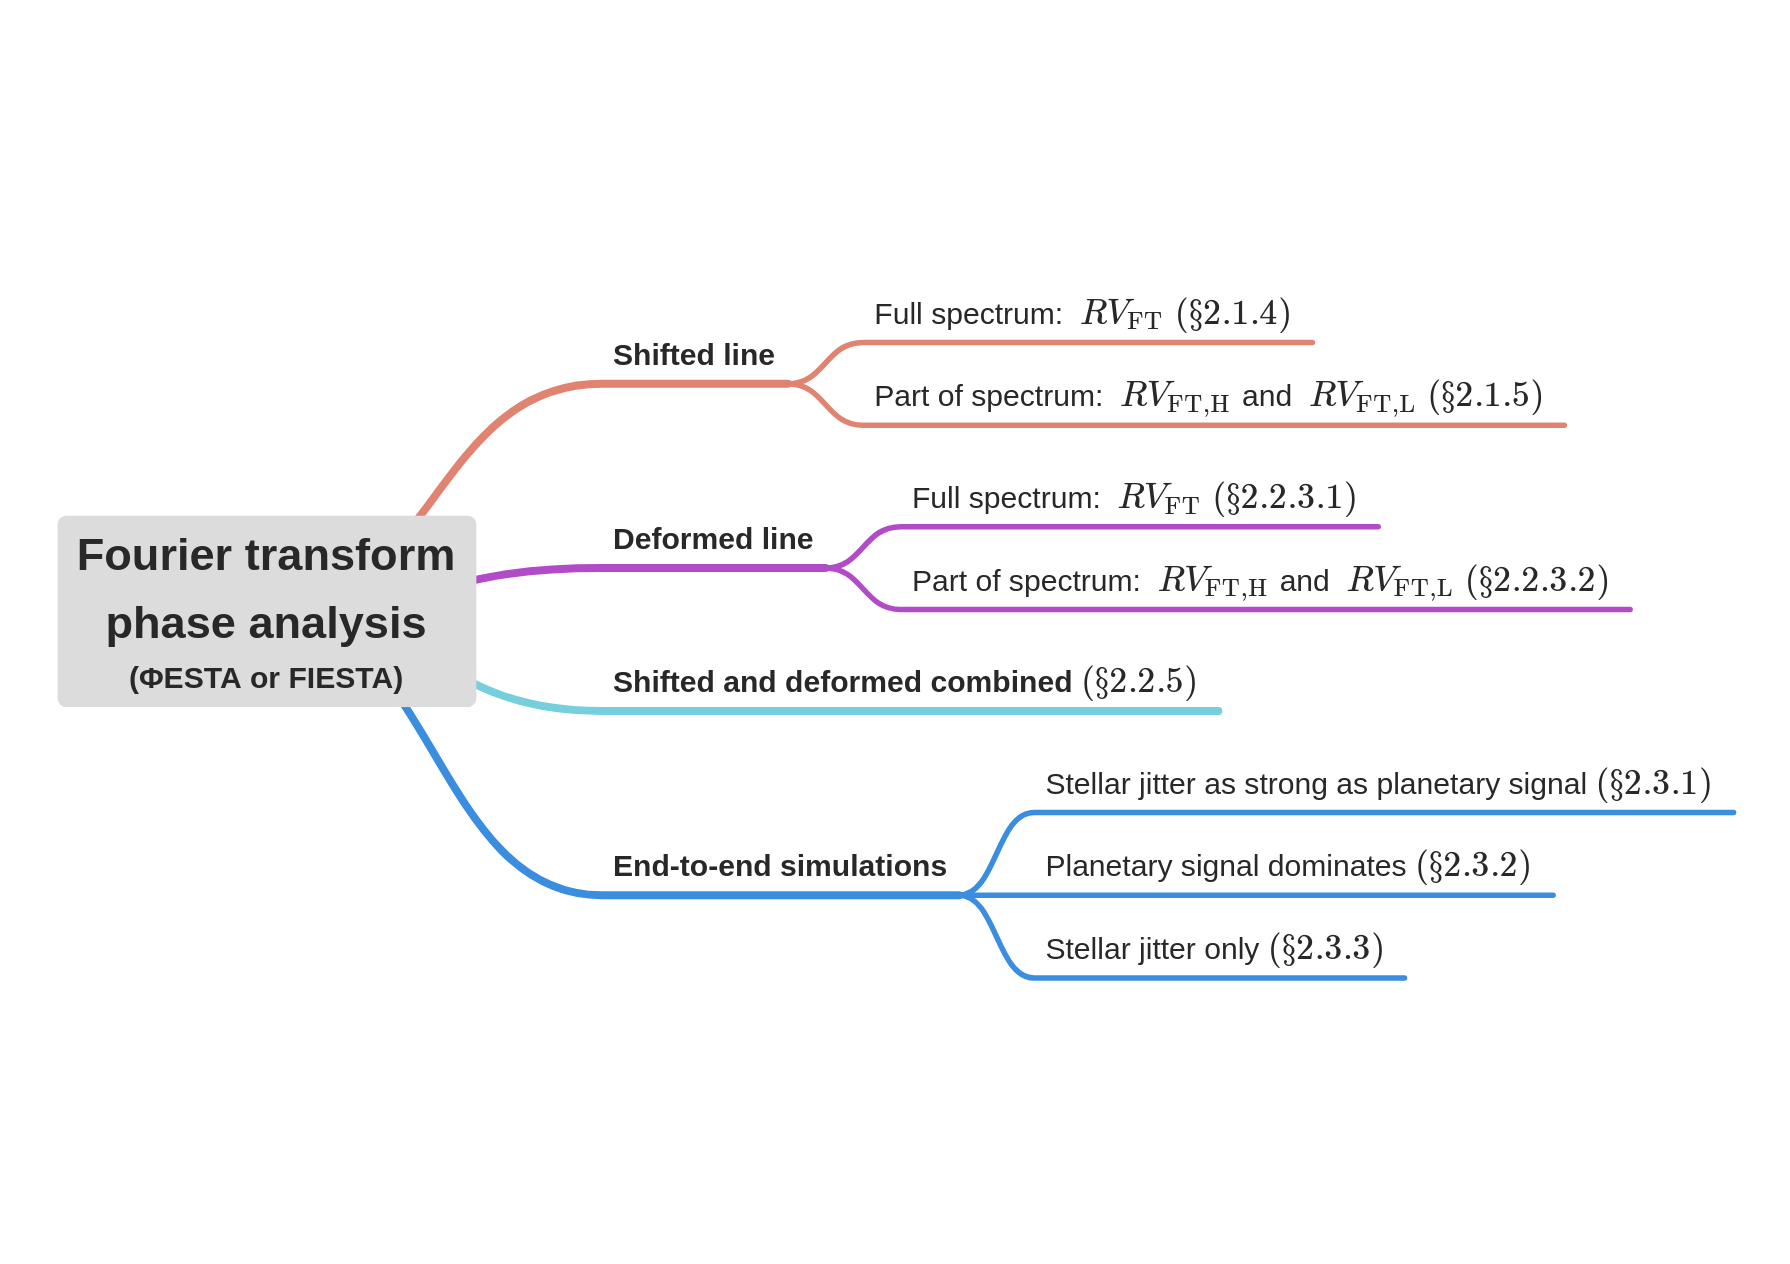
\includegraphics[width = 1.0 \linewidth]
{./Figures/Methods/Thinkmap.png}
\caption[Simulation map]
{Roadmap of Fourier transform phase analysis on simulated data.}
\label{fig:simulation_map}
\end{figure} 
%-------------

%%----------------------------------------------------------------------------------------	
\pagebreak
%%----------------------------------------------------------------------------------------	

\section{Phase analysis of Fourier transform for the measurement of line shift}
\label{\thesection}
\label{ch:FT_line_shift}

The translation of a function (in our case a spectral line profile) can be examined in both its original real
space, and in its Fourier transformed space. Because Fourier transform is often used to handle time domain data,
a shift in real space can be variously described as either time shifting or translation. In this chapter 
we will use ``time shifting'', ``translation'' and ``velocity shifting'' interchangeably to refer to a shift of a function in real space. We will refer to Fourier transformed functions as being in the ``frequency domain'' regardless of whether they have actual dimensions of 1/time, 1/length or 1/velocity.

\subsection{Translation property of Fourier transform}

Let us consider a function $h(x)$ as a signal $f(x)$ delayed (or shifted) by an amount $x_0$:
\begin{equation}
	h(x) = f(x-x_0).
\label{eq:FT1}
\end{equation}
In the frequency domain, we will then have 
\begin{equation}
	\hat{h}(\xi) = e^{-2 \pi ix_0 \xi} \hat{f}(\xi),
\label{eq:FT2}
\end{equation}
where the circumflex denotes the Fourier transform of a function, i.e.
\begin{equation}
	\hat{f}(\xi) = \int_{-\infty}^{\infty} f(x) e^{-2 \pi ix \xi} dx.
\label{eq:FT3}
\end{equation}
E.q.~\ref{eq:FT2} means that while the power spectrum remains unchanged for shifted signals, i.e. $\mid \hat{h}(\xi)\mid ^2 = \mid\hat{f}(\xi)\mid^2$, the phases $\phi(\xi)$, defined as the argument of the Fourier representation $\hat{f}(\xi)$:  $\operatorname{Arz}(\hat{f}(\xi))$, have changed because of the additional term $e^{-2 \pi ix_0 \xi}$. The extra phases $\Delta \phi(\xi)$ added are: 
\begin{equation}
	\Delta \phi(\xi) = -2 \pi x_0 \xi.
\label{eq:PhaseShift}
\end{equation}

\subsection{Intuitive explanation}

An intuitive, but equally quantitative way, to see how E.q.\ref{eq:PhaseShift} holds is as follows. The Fourier transform decomposes the function $f(x)$ into a frequency representation $\hat{f}(\xi)$, accompanied by the orthogonal basis $e^{2 \pi ix \xi}$, as in the form of inverse Fourier transform: 
\begin{equation}
	f(x) = \int_{-\infty}^{\infty} \hat{f}(\xi) e^{2 \pi ix \xi} d\xi. 
\end{equation}
Shifting $f(x)$ by $x_0$ is equivalent to shifting \textit{all} the orthogonal basis functions by $x_0$, which then become $e^{2 \pi i(x-x_0) \xi} = e^{2 \pi i x \xi} \cdot e^{-2 \pi ix_0 \xi}$. This is how the additional term $e^{-2 \pi ix_0 \xi}$ in Eq.~\ref{eq:FT2} arises -- it quantifies the phase difference for a shifted function. 

An even more intuitive but less quantitative way to envision the relation between a shift of the signal and a phase difference is to imagine any real continuous function is a sum of sines and cosines. Changing the phase angle in the sines and cosines results in shifts in the function. 

The power spectrum of such a shifted function remains the same because shifting the signal as a whole doesn't add or remove any frequency components. 


\subsection{Practical Use}

From Eq.~\ref{eq:PhaseShift}, we see that the phase shift $\Delta \phi(\xi)$ is proportional to the frequency $\xi$ with a constant gradient or slope
\begin{equation}
	\dv{(\Delta \phi)}{\xi} = -2 \pi x_0
\label{eq:gradient}
\end{equation}
where $\Delta$ is used to refer to the phase difference between a shifted line profile and an unshifted (referenced) line profile, while the derivative refers to the response of $\Delta \phi(\xi)$ to $\xi$. $\Delta \phi(\xi)$ is measured as the change in phases $\operatorname{Arz}(\hat{h}(\xi)) - \operatorname{Arz}(\hat{f}(\xi))$. Then a linear regression model can be fit to a plot of $\Delta \phi(\xi)$ versus $\xi$ (Fig.~\ref{fig:FT}) to enable measurement of the bulk shift between two line profiles $x_0$. 

%-------------
\begin{figure}[tbp]
\centering
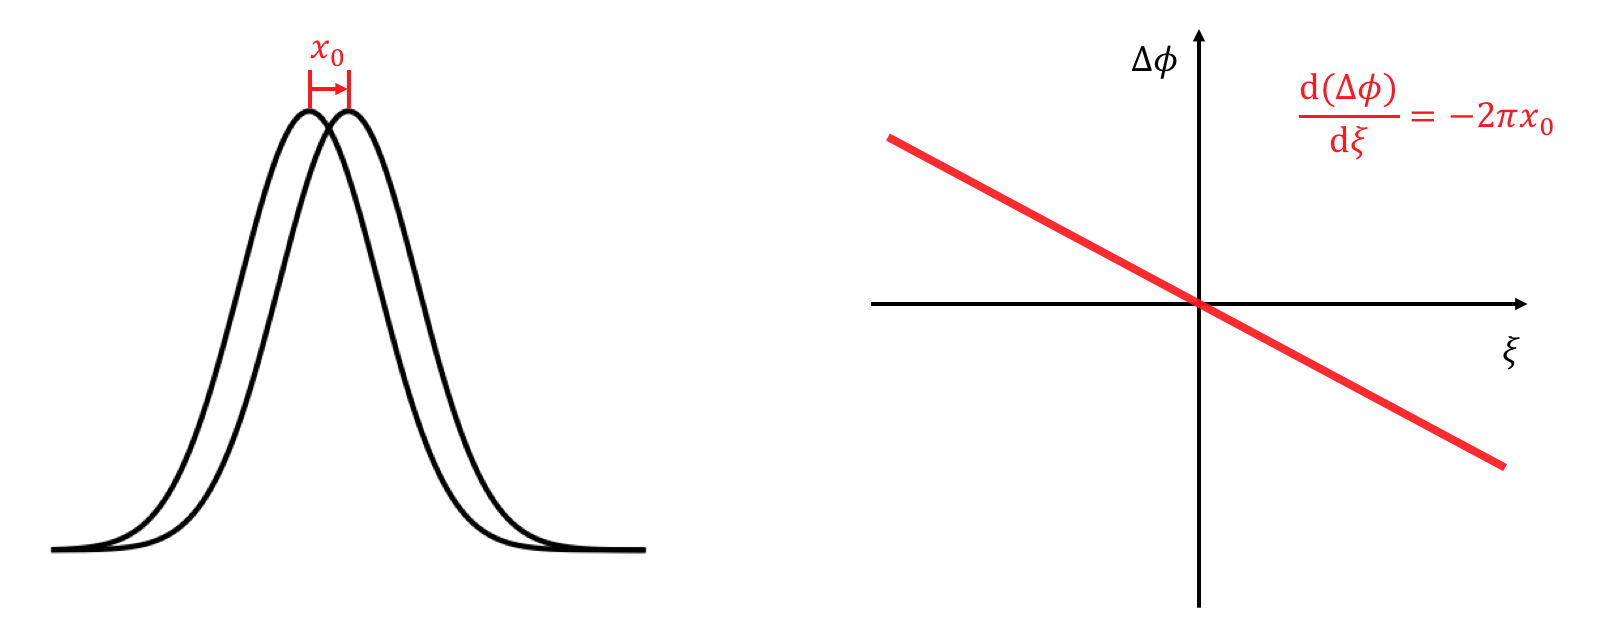
\includegraphics[width = 0.99 \linewidth]
{./Figures/Methods/FT.png}
\caption[Translation property of Fourier transform]
{The left panel shows a signal (or a spectral line profile in the following context) shifted by an amount $x_0$. 
The right panel is the differential phase spectral density diagram (i.e. differential phase spectrum). 
The model shows the phase difference between two shifted signals $\Delta \phi(\xi)$ and the frequency $\xi$ are linearly correlated. Its slope $-2 \pi x_0$ contains information of the amount of signal shift in time domain.}
\label{fig:FT}
\end{figure} 
%-------------

By analogy with the definition of power spectrum, we describe $\phi(\xi)$ as the \textbf{phase spectrum} and hence $\Delta \phi(\xi)$ as the \textbf{differential phase spectrum}. In this approach, an analysis of the phase shift in the frequency domain of the Fourier components of a line profile will provide a means of measuring a bulk line shift in real space. We therefore name our method \textbf{FourIEr \textit{phase} SpecTrum Analysis} ($\mathit{\Phi}$ESTA or FIESTA). 

%----------------------------------------------------------------------------------------	

\subsection{Initial tests to obtain $RV_\text{FT}$}
\label{sec:Initial_tests}

We performed an initial test to determine that we can correctly recover known shifts of a line profile using $\mathit{\Phi}$ESTA. We generated a spectral line profile based on the cross-correlation function of observed HARPS spectra with the software SOAP 2.0 \cite{Dumusque2014SOAP}. This was replicated 100 times, with a very small amount of 
noise (equivalent to a S/N = 10,000) injected in each of the line profiles. These profiles were then
subjected to radial velocity shifts evenly spaced between 0 and 10\,m/s (Fig.~\ref{fig:line_profiles12}). 

%-------------
\begin{figure}[tbp]
    \begin{subfigure}[b]{0.49\textwidth}
        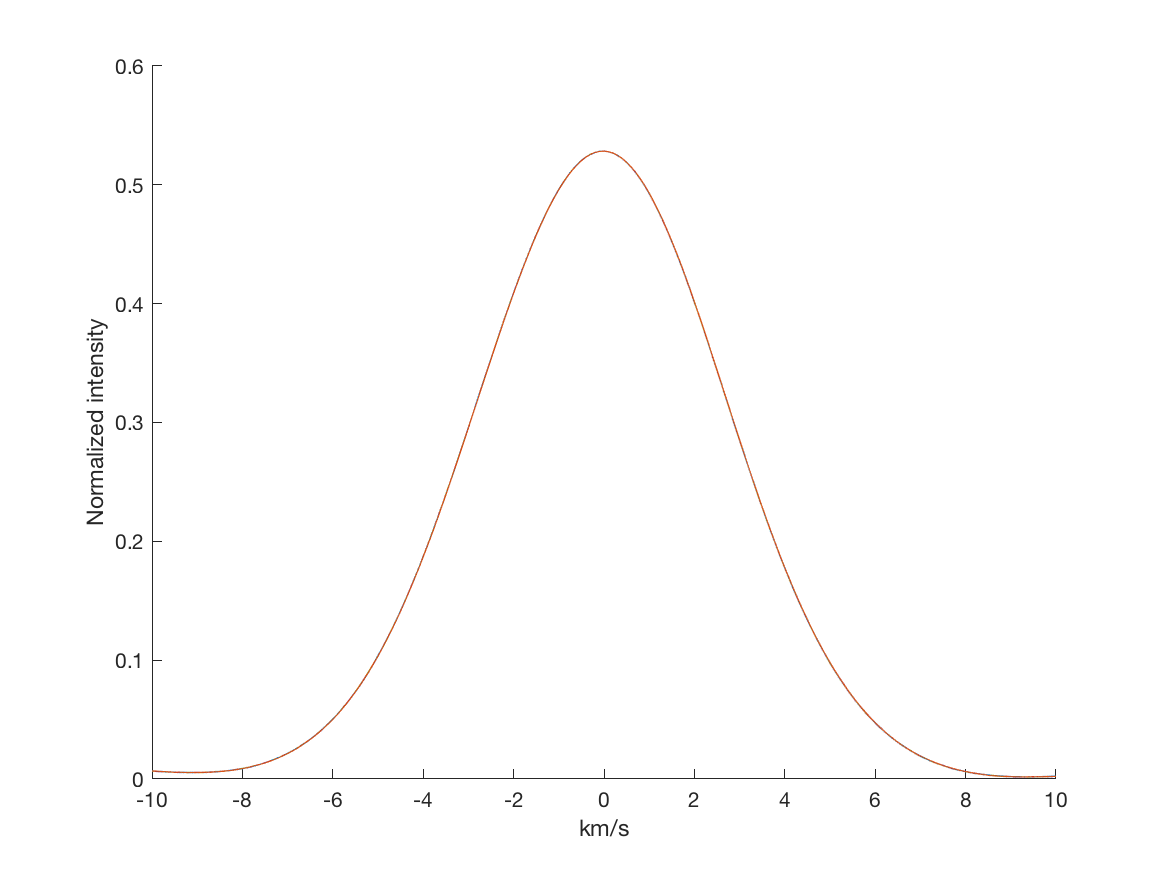
\includegraphics[width=\textwidth]{./Figures/Methods/1-Line_Profile.png}
        \caption{Line profile (stacked)}
        \label{fig:line_profiles}
    \end{subfigure}
	~
    \begin{subfigure}[b]{0.49\textwidth}
        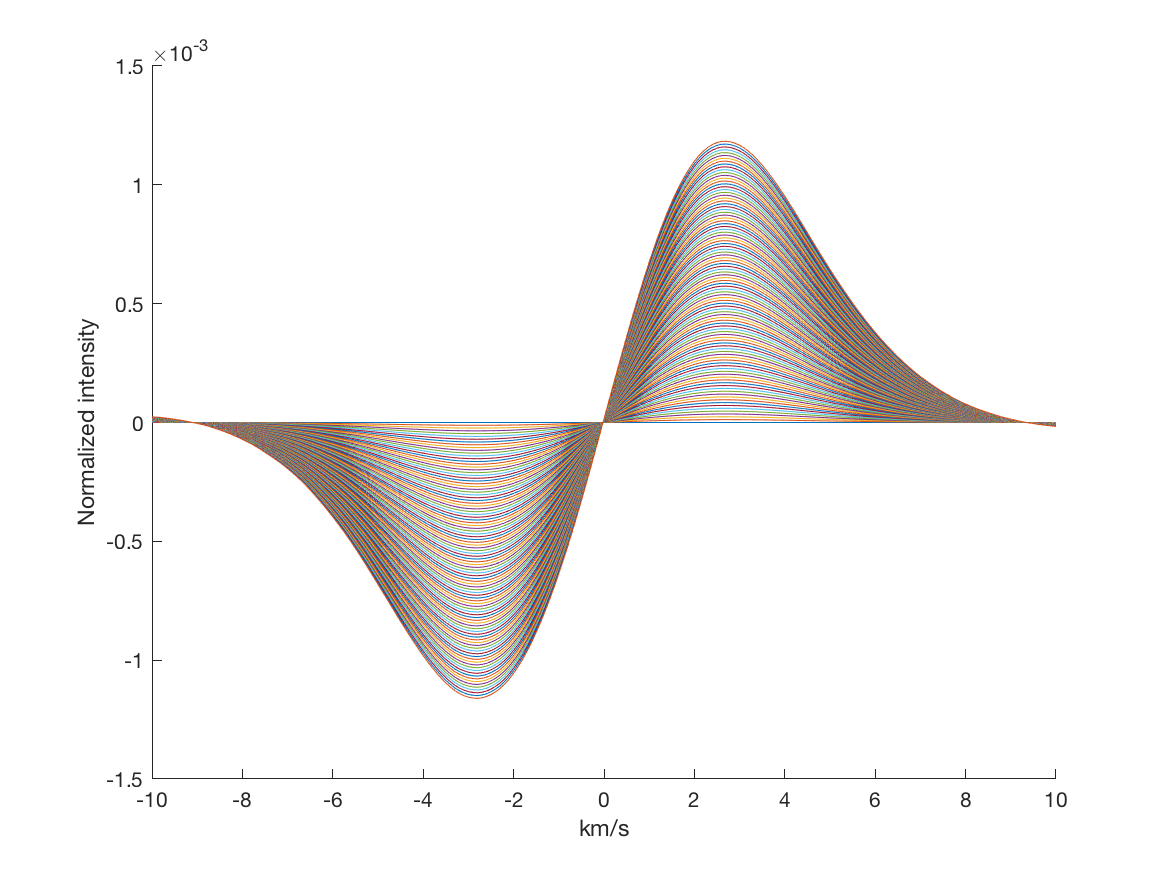
\includegraphics[width=\textwidth]{./Figures/Methods/1-Differential_line_Profile.png}
        \caption{Differential line profile}
        \label{fig:differential_line_profiles}
    \end{subfigure}	
    
    \caption[100 shifted HARPS-like line profiles]{(a) the shifted line profiles plotted on top of each other, showing that the 0-10\,m/s shifts are very small compared to the line profile width. (b) the shifted line profiles with the unshifted line profile subtracted from each. Note that for the sake of clarity, the differential line profiles are plotted noise-free and only 10 out of 100 profiles are displayed.}
\label{fig:line_profiles12}
\end{figure}	
%-------------

The Fourier transform of these 100 spectral line profiles divides the information into two parts: (1) the power spectra (Fig.~\ref{fig:power_spectrum}) and (2) the phase spectra (shown in Fig.~\ref{fig:dps} as the differential phase spectra -- the difference relative to the phase spectrum of the unshifted line profile rather than its own derivative). We see that most information is concentrated towards the centre of the power spectrum (i.e. the lower frequency range), and as expected, the differential phase spectra are mostly linear, consistent with the theory demonstrated in Fig.~\ref{fig:FT}. Deviations from linearity come from the noise that we injected, which will be discussed later. 

%-------------
\begin{figure}[tbp]	
    \begin{subfigure}[b]{0.49\textwidth}
        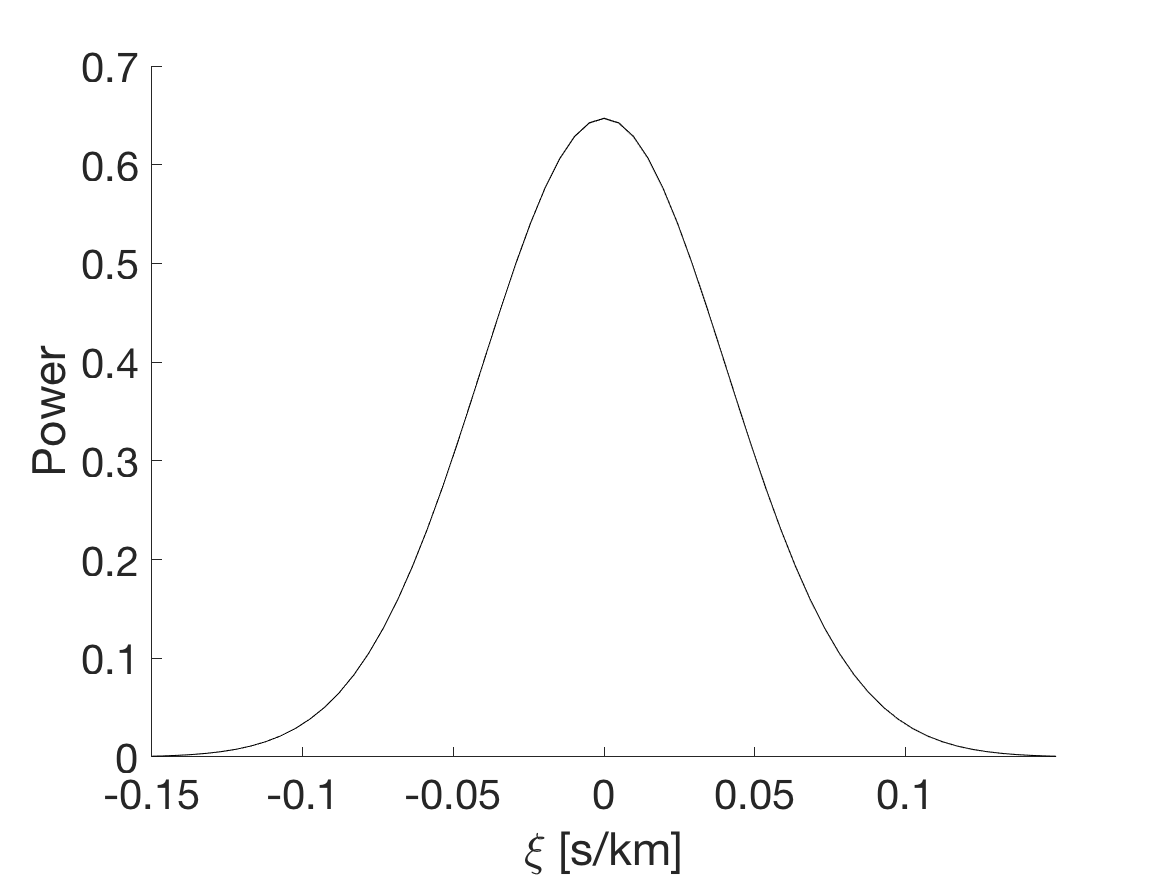
\includegraphics[width=\textwidth]{./Figures/Methods/2-FT_power.png}
        \caption{Power spectrum (stacked)}
        \label{fig:power_spectrum}
    \end{subfigure}
	~
    \begin{subfigure}[b]{0.49\textwidth}
        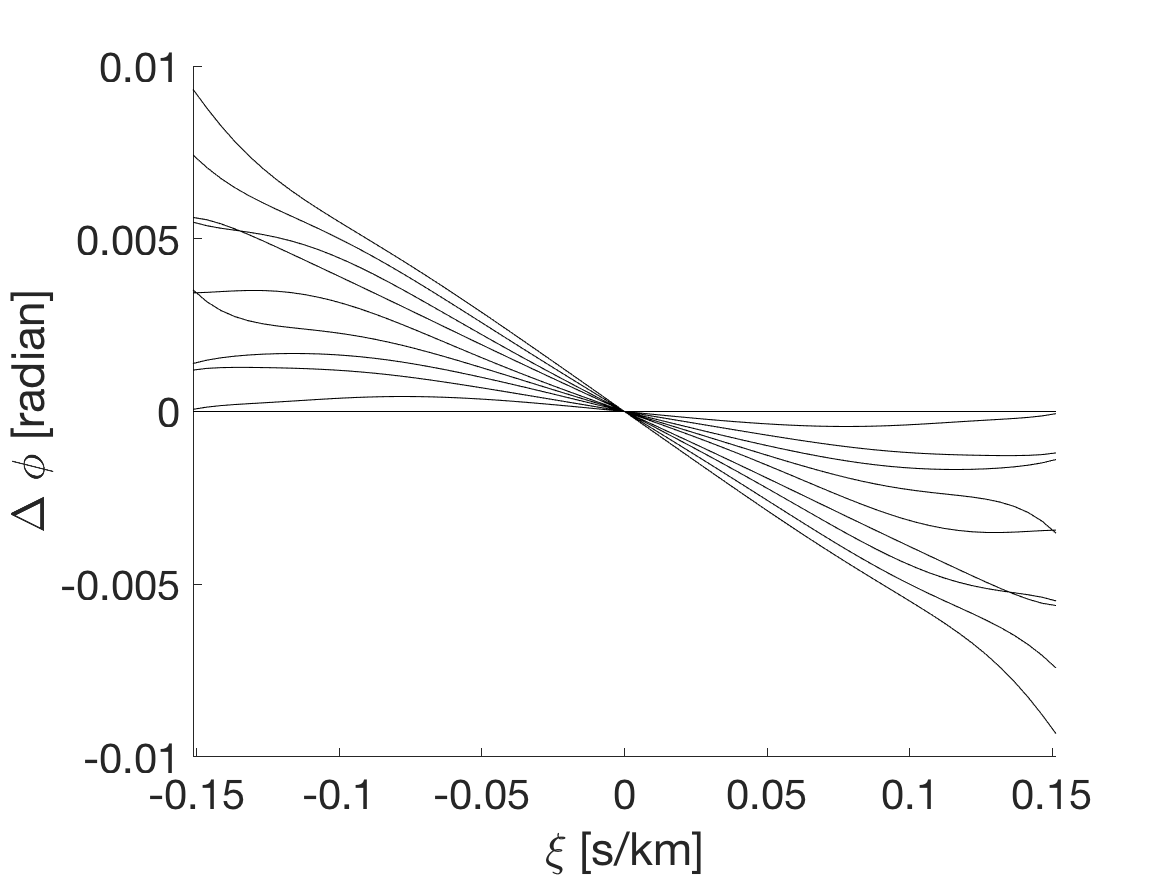
\includegraphics[width=\textwidth]{./Figures/Methods/4-Relative_phase_angle.png}
        \caption{Differential phase spectrum}
        \label{fig:dps}
    \end{subfigure}	
    \caption[Fourier transform of 100 shifted line profiles]
    {The Fourier transform of these shifted line profile divides the information in each into (a) their power spectra and (b) their phase spectra (here plotted differential compared to that of the unshifted profile). A line shift in the time domain produces an unchanged power spectrum in the frequency domain. It does, however, produce phase shifts which we see as linear trends in the differential phase spectra as a function of frequency. Only 10 out of 100 differential phase spectra are displayed. The differential phase spectrum can be sub-divided into higher frequency range (H) and lower frequency range (L). The $\varnothing$ region contains little power and frequency information and thus not used. We derive $RV_\text{FT}$ from the full spectrum (except $\varnothing$), $RV_\text{FT,H}$ from the higher frequency range and $RV_\text{FT,L}$ from the lower frequency range.}
\label{fig:FT_process}
\end{figure}    
%-------------

The slope of each differential phase spectrum indicates the shift of each line profile relative to the unshifted one. For a linear regression fitting, each frequency sample on the differential phase spectrum is weighted by the amplitude of the power, meaning the lower frequencies receive more weights. We calculate the radial velocity shift for each shifted line profile using two methods: (1) $\mathit{\Phi}$ESTA to determine $RV_\text{FT}$; (2) traditional measurement of the line centroid by fitting a Gaussian function to each line profile that delivers $RV_\text{Gaussian}$. 

We then compare both $RV_\text{FT}$ and $RV_\text{Gaussian}$ with the known input line shift. Fig.~\ref{fig:rv_recovery} reveals the expected 1:1 correlation between the input radial velocity shift and the output -- the line of best fit of a linear regression model presents a slope of $0.996\pm0.006$ with 95\% confidence bounds for both $RV_\text{FT}$ and $RV_\text{Gaussian}$. The standard deviation of the residuals are both $\sigma_\text{FT} = \sigma_\text{Gaussian} = 0.08$ m/s, identical up to two decimal places, indicating the expected radial velocities are consistently obtained by both methods. In fact, the almost overlapping residuals in Fig.~\ref{fig:rv_recovery} middle panel means that the two methods are so coherently different from the input radial velocity (by small amounts) that this scatter must come from the photon noise intrinsic to the simulated line profiles rather than the methods themselves. 

%-------------
\begin{figure}[tbp]
\centering
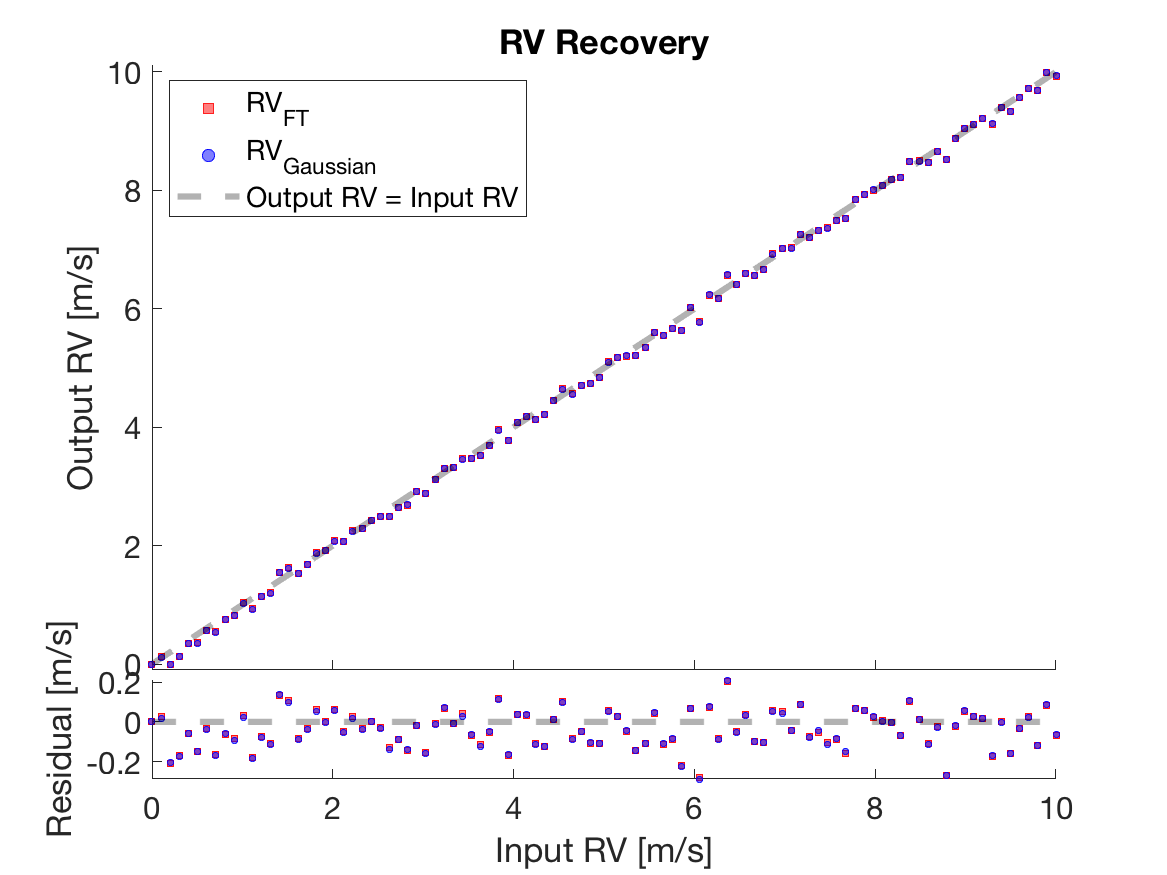
\includegraphics[width = 0.7 \linewidth]
{./Figures/Methods/5-LINE_SHIFT_ONLY.png}
\caption[Radial velocity recovery]
{Radial velocity recovery of line shifts with both methods: Fourier transform and Gaussian fit. Top: $RV_\text{FT}$ and $RV_\text{Gaussian}$ plotted against the input radial velocity shifts. Middle: residuals as $RV_\text{FT}$ and $RV_\text{Gaussian}$ subtracted by the input radial velocity shifts. Bottom: $\Delta RV$ defined as the difference between $RV_\text{FT}$ and $RV_\text{Gaussian}$, showing the highly consistency between each other. Note that axes scales are different across the subplots; errorbars are estimated to be the size of scatter 0.08~m/s but are not plotted for clarity.}
\label{fig:rv_recovery}
\end{figure} 
%-------------
\FloatBarrier

{\em CGT: How do these comare which what you'd expect from the S/N and the intrinsic line width (should say at some int what the intrinsic line width is}.


%----------------------------------------------------------------------------------------	

\subsection{Further tests to obtain $RV_\text{FT,H}$ and $RV_\text{FT,L}$}
\label{sec:Further_tests}

Let's recall the justification of measuring a line shift in its Fourier space -- the shifting of a line (or a function), when viewed as shifting the sum of its Fourier basis functions (or any other basis functions), has equally the same amount of shift on every basis function, which can be measured as a phase shift in the Fourier phase spectrum. That is to say, utilising only part of the phase spectrum will also return the correct shift of a line profile, although it utilises less information. The motivation of this will be discussed in \S\ref{sec:FT_ld} when we look at line profile deformations. 

We divide the whole frequency range available into two parts (Fig.~\ref{fig:FT_process}) -- a lower frequency range (i.e. apply a low-pass filter) and a higher frequency range (i.e. apply a high-pass filter). The dividing frequency $\xi_{HL}$ can be chosen arbitrarily for the time being, for example, such that both the lower and higher frequency ranges take up half of the power spectrum $P(\xi)$:
\begin{equation}
	\int_{\xi_{L}=0}^{\xi_{HL}} P(\xi) d\xi = \int_{\xi_{HL}}^{\xi_{H}} P(\xi) d\xi. 
\end{equation}
We assume here that the integration of the power spectrum measures the amount of ``information" in the original line profile, so that we would put equal trust on the radial velocities obtained from the lower and higher frequencies (namely $RV_\text{FT,L}$ and $RV_\text{FT,H}$, or $RV_\text{FT,H/L}$ for both). In addition, a cut-off frequency $\xi_{H}$ is applied to the upper boundary of the high-pass filter (so is $-\xi_{H}$ on the negative part; but since it can be easily proved that the phase spectrum $\phi(\xi)$ of any function $f(x)$ is antisymmetric, i.e. $\phi(\xi) = -\phi(-\xi)$, therefore the differential phase spectrum $\Delta \phi(\xi)$ is also antisymmetric and we can simply focus on the non-negative part of the spectrum). Frequencies higher than $\xi_{H}$ hardly contributes to the shape of the line profile as the power $P(\xi)$ converges to zero and thus not used. The cut-off frequency should be chosen large enough so that the frequency range to be used extracts the most information from the power spectrum and phase spectrum, but not as far up as going beyond the noise level. Empirically, it is safe to choose $\xi_{H}$ where $P(\xi)$ drops to $0.01\%$ of max$\{P(\xi)\}$ for a high S/N = 10,000, as in our simulation. Lower S/N observations should be applied with a smaller $\xi_{H}$ accordingly. 

We presented in Fig.~\ref{fig:rv_recovery} an accurate recovery of the radial velocity shifts given by $RV_\text{FT}$, for which the full range of frequencies were used; For exactly the same set of data but sub-divided into two frequency ranges, we plot $RV_\text{FT,H/L}$ against the input radial velocities (Fig.~\ref{fig:rv_recovery_LH}), which still delivers a good 1:1 relation. The line of best fit presents a slope of $1.003\pm0.010$ for $RV_\text{FT,H}$ and $0.991\pm0.011$ for $RV_\text{FT,L}$ respectively, with 95\% confidence bounds. The scatter of the residuals are $\sigma_\text{FT,H} = 0.21$ m/s and $\sigma_\text{FT,L} = 0.19$ m/s. First, we note that $\sigma_\text{FT,H/L} > \sigma_\text{FT}$~(=0.08~m/s), this is because both $RV_\text{FT,H}$ and $RV_\text{FT,L}$ are only derived from nearly half of the total ``information" in the Fourier space. Second, we note that $\sigma_\text{FT,H}$ and $\sigma_\text{FT,L}$ only differ by a small amount, offering similar performance in recovering the radial velocity shifts, and this is because they are derived from roughly equal amount of ``information". 
%The fact that $\sigma_\text{FT,H}$ is slightly larger may be because higher frequency modes are more likely to be subjected to stochastic behaviours such as shot noise. See the following subsection for a related discussion of introducing a cut-off frequency.

%seemingly contradicting with the expectation that  We think this may be because higher frequency modes are more likely to be subjected to stochastic behaviours other than the line deformation arising from stellar variability generated in the SOAP model. For example, the fluctuations of photon levels on the stellar spectrum are mainly described by high frequency modes. {\em jzhao: Have I made myself clear here?}

%-------------
\begin{figure}[tbp]
\centering
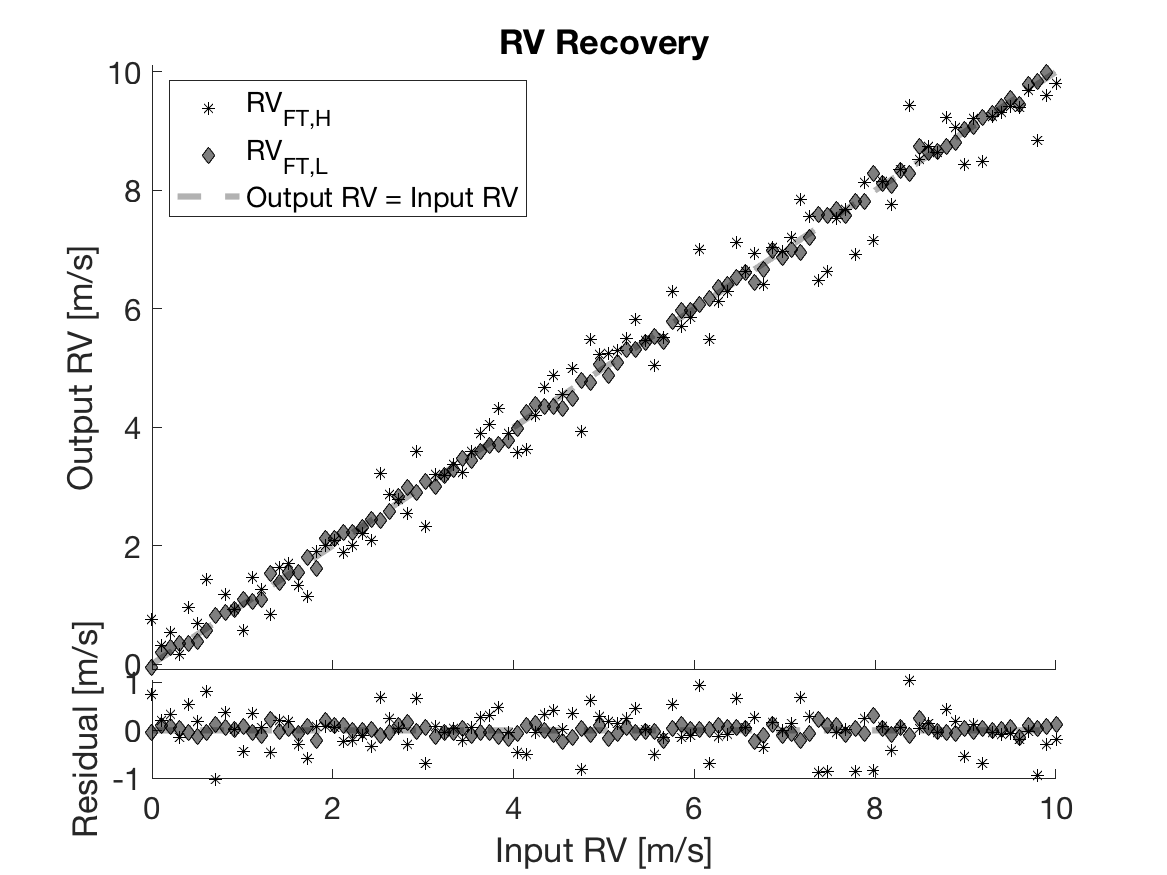
\includegraphics[width = 0.7 \linewidth]
{./Figures/Methods/5-LINE_SHIFT_ONLY-HL.png}
\caption[Low-pass and high-pass radial velocities]
{Radial velocity recovery of line shifts with low-pass and high-pass filters. Errorbars are estimated to be around 0.2~m/s but not plotted for clarity.}
\label{fig:rv_recovery_LH}
\end{figure} 
%-------------
\FloatBarrier

%----------------------------------------------------------------------------------------
\subsection{Cut-off frequency}
\label{sec:noise}

We mentioned in \S\ref{sec:Initial_tests} that deviation from linearity in the differential phase spectrum may arise from the photon noise injected in the simulated line profiles, and we also introduced a cut-off frequency $\xi_{H}$ in \S\ref{sec:Further_tests} to avoid dealing with frequencies higher than $\xi_{H}$. The motivation of these becomes clear on the frequency representation $\hat{f}(\xi)$ of a line profile in a complex plane (a.k.a. the Argand plane; Fig.~\ref{fig:FT_compelx_plane}). 

We see a scattered plot because the frequencies $\xi$ are discretely sampled. $\hat{f}(\xi)$ of noise-free and S/N = 10,000 are plotted for the same sampling of frequencies. The argument of $\hat{f}(\xi)$ returns the phase angle and the square of its absolute value (or modulus) returns the power. $\hat{f}(\xi)$ at larger power (i.e. those far from the origin as viewed in Fig.~\ref{fig:FT_compelx_plane} left) is barely affected in the presence of noise; $\hat{f}(\xi)$ at lower power (i.e. those distributed in the vicinity of the origin as viewed in Fig.~\ref{fig:FT_compelx_plane} right) are more affected by noise, as a slight displacement of $\hat{f}(\xi)$ in the complex plane means a considerable change in the phase angle. As a result, at S/N = 10,000, the distribution of $\hat{f}(\xi)$ in the zoomed-in complex plane is more scattered than a noise-free scenario, and the phase angle measurement is not as reliable as for $\hat{f}(\xi)$ with larger powers. This justifies using the Fourier transform spectral power as a weight, and introducing a cut-off frequency for shift measurements. 

Another potential reason to introduce the cut-off frequency is the periodicity of the basis functions in a Fourier transform. The basis functions $e^{-2 \pi ix_0 \xi}$ repeat themselves at the periods of $1/\xi$, making measuring the shift in the time domain (velocity domain for line profiles) larger than the order of $1/\xi$ degenerate (i.e. the shifts of $x_0+k/\xi$ for $k\in\mathbb{Z}$ become indistinguishable). Nevertheless for cut-off frequency $\xi \sim 0.15$ s/km, such a shift needs to be more than $1/\xi\sim6.7$~km/s to fail the measurement, while the radial velocities induced by planets are usually at m/s amplitudes and will not be a concern.

%-------------
\begin{figure}[tbp]
\centering
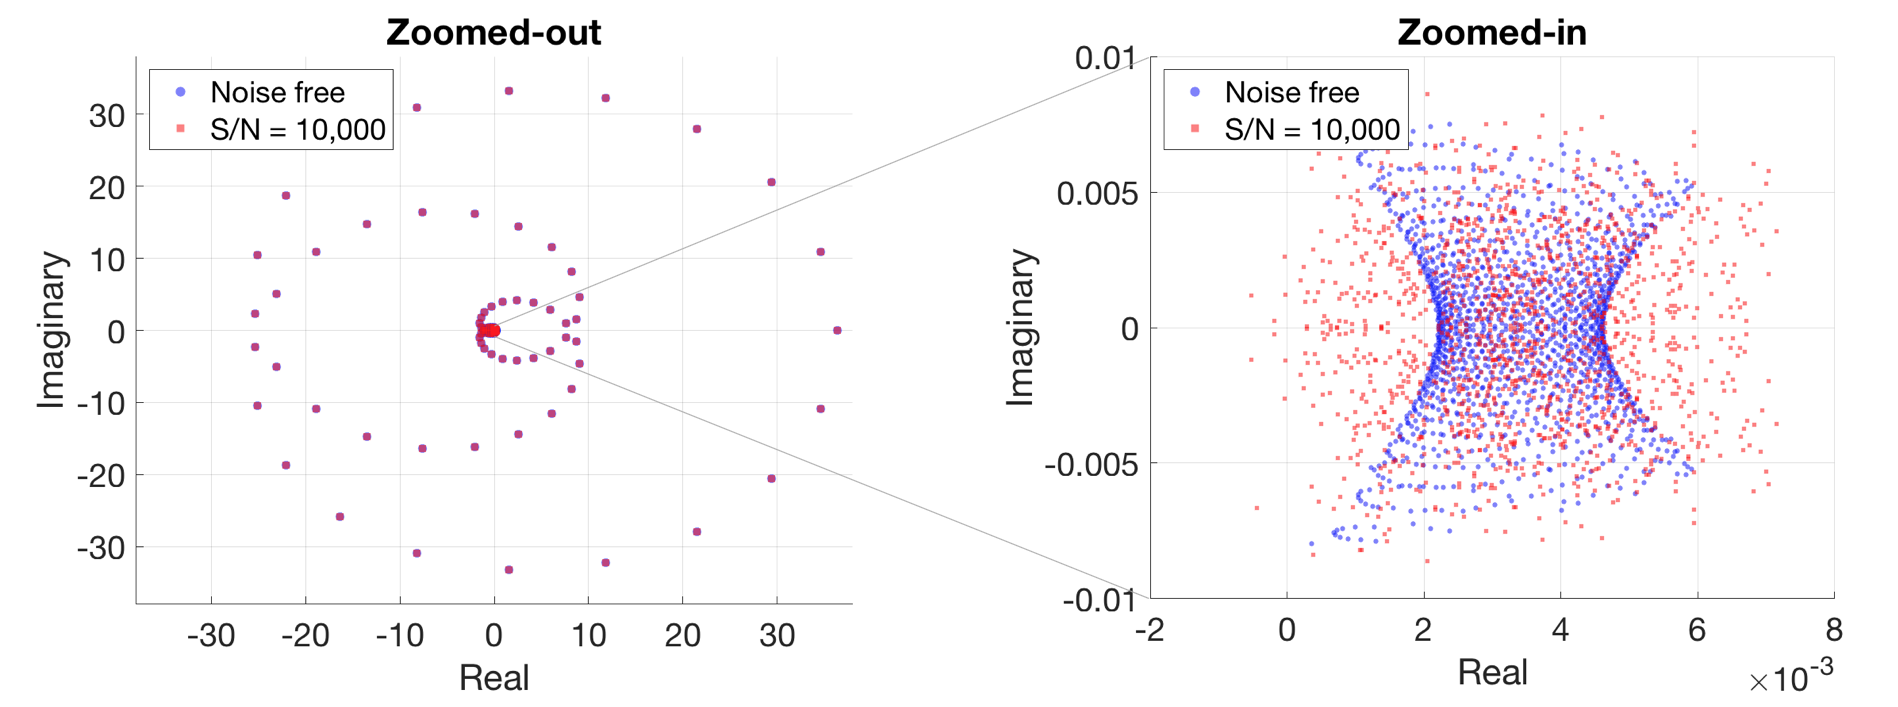
\includegraphics[width = 0.99 \linewidth]
{./Figures/Methods/7-complex_plane.png}
\caption[The frequency representation $\hat{f}(\xi)$ of a line profile in a complex plane]
{The frequency representation $\hat{f}(\xi)$ of a line profile in a complex plane. The right panel is a zoom-in of the left near the origin. For the same sampling of frequencies, $\hat{f}(\xi)$ on the complex plane is less defined or more scattered in the presence of noise, making the measurement of the phase angle with a small amplitude far less reliable than measured without noise. This motivates us to come up with a cut-off frequency to relinquish $\hat{f}(\xi)$ higher than the threshold frequency, which is equivalent to abandoning amplitudes smaller than a threshold.}
\label{fig:FT_compelx_plane}
\end{figure} 
%-------------

\FloatBarrier

%This is because we only use part of the information from the original line profile -- both because we utilise a limited range of the differential phase spectra, and because we use only the phase spectra to measure this shift (ignoring the power spectra), while the total information in the original shifted line profile is contained in the combination of the power and phase spectra. 
%
%{\em CGT: This needs more work. You need to show the region you are not using to explain why you choose a more linited range, and
%then say why you chose that more limited range and justify it. Don't just say "higher frequency}.
%
%In fact, higher frequency range becomes useless 
%as the interpretation of Fourier transform in high frequencies is dominated by noise and does not represent the 
%intrinsic shift of the line profile any more. As a result, linearity of phase spectrum breaks down in higher frequencies. 
%The range of ``useful" frequencies will depend on the amount of noise (i.e. S/N). 

%----------------------------------------------------------------------------------------	

\subsection{Conclusion}
In this section, we have introduced a new method for measuring radial velocities -- Fourier phase spectrum analysis (a.k.a $\mathit{\Phi}$ESTA or FIESTA). We tested this method on shifting a simulated line profile. It concludes that the newly proposed technique $\mathit{\Phi}$ESTA is able to measure a radial velocity shift at similarly high precision as fitting a line centroid by a Gaussian profile, and thus provides an alternative to the traditional means of obtaining the radial velocities. 

In a broader context, this method will be applicable to measuring shifts of any pattern, and can also be extended to higher dimensions. In this thesis, we primarily focus on its use to measure radial velocity shifts in spectral line profiles.

%, and especially whether the Fourier transform phase velocity is more robust against the influence of changes in line deformation than traditional techniques.

\pagebreak
%----------------------------------------------------------------------------------------	
%----------------------------------------------------------------------------------------	

\section{Using the Fourier transform to probe line deformation}
\label{\thesection}
\label{sec:FT_ld}

In \S~\ref{ch:FT_line_shift}, we showed that $\mathit{\Phi}$ESTA correctly measures the actual line profile shifts due to a bulk motion of the emitting star. In this section, we test whether this method is robust against spurious apparent radial velocity shifts produced by changes in the line profile shape.

%----------------------------------------------------------------------------------------	

\subsection{Theory}
\label{sec:LD_Theory}

For a line profile shifted by a small amount $x_0$, the same shift $x_0$ applies to \textit{all} of its basis functions. Where a line profile is changed or deformed (as opposed to simply shifted), $x_0$ becomes frequency dependent. That is to say, basis functions at different frequencies would be shifted by different amounts to produce shape changes (e.g. skewness, kurtosis and higher order terms) in the line profile. Therefore we modify the translation property of Fourier transform by rewriting $x_0$ as $x_0(\xi)$ in Eq.~\ref{eq:PhaseShift}:
\begin{equation}
	\Delta \phi(\xi) = -2 \pi x_0(\xi) \xi.
\label{eq:PhaseShift2_LPD}
\end{equation}
%As a result, the local gradient of the differential phase spectrum, instead of $-2 \pi x_0$ in the case of no line profile deformation, becomes 
%\begin{equation}
%	\dv{(\Delta \phi)}{\xi} = -2 \pi (x_0 + \dv{x_0}{\xi}).
%\label{eq:PhaseShift3_LPD}
%\end{equation}
%Note that the dependency of $\xi$ has been taken out of $\Delta \phi(\xi)$ and 
%$x_0(\xi)$ in writing the differential equation above. 
$x_0(\xi)$ contains all the information of how much a line is deformed (as well as shifted). In other words, $x_0(\xi)$ can parametrize the line deformation. In principle, we could derive $x_0(\xi)$ from the expression above to further seek to understand which frequency modes are related to stellar variability, as distinct from frequency modes responding to a bulk shift of a line profile. We opt for a simplistic approach instead -- use an \textit{averaged} shift $\overline{x_0(\xi)}$ to describe an overall shift of various frequency modes and rewrite Eq.~\ref{eq:PhaseShift2_LPD} as 
\begin{equation}
	\Delta \phi(\xi) = -2 \pi \overline{x_0(\xi)} \xi
\label{eq:PhaseShift2_LPD_ave}
\end{equation}
where $\overline{x_0(\xi)}$ is treated as a constant for the range of frequencies of interest. 

We may interpret E.q.~\ref{eq:PhaseShift2_LPD_ave} in two ways: (1) within a narrow frequency range, $x_0(\xi)$ is approximately a constant (hence labelled as $\overline{x_0(\xi)}$) and so the shift is proportional to the local gradient of the differential phase spectrum; (2) for a wide range of continuous frequencies, $\overline{x_0(\xi)}$ can be regarded as an effective line shift, and then we can study such shifts in the lower frequency range versus the higher frequency range the same way we dealt with a pure line shift in \S\ref{ch:FT_line_shift}. 

%numerically solve the differential equation (either Eq.~\ref{eq:PhaseShift2_LPD} or Eq.~\ref{eq:PhaseShift3_LPD}) based on the measured $\Delta \phi$ or local gradient d$(\Delta \phi)$/d$\xi$ to obtain $x_0(\xi)$, 

%----------------------------------------------------------------------------------------	

\subsection{SOAP simulations}
\label{sec:Simulations}

In \S~\ref{ch:FT_line_shift}, we used the SOAP simulator to generate a line profile that resembles the HARPS observation to study a line shift in the Fourier space. In this section, we instead use SOAP~2.0 to study line deformations arising from starspots. 

We injected three spots with different longitudes, latitudes and sizes (parameters were arbitrarily chosen and specified in Table~\ref{table:spot_configurations}) to model an emitting star. The spectral line profile is therefore deformed in the presence of spots. Such intrinsic line variabilities produce apparent radial velocities shifts (a.k.a. jitter) as a star rotates (also as spots themselves evolve with time, but such a feature is not automatically implemented in the SOAP simulator and we do not include this feature). The jitter amplitude depends on, but not limited to, the sizes and the positions of starspots; the three spots that we use present an amplitude of roughly 2~m/s. The same spot configuration is used in all simulations throughout the chapter. 

We generated 100 cross-correlation functions for the resulting  deformed line profiles evenly sampled throughout one rotation period of the star (Fig.~\ref{fig:line_profiles_deformation}). A very small amount of noise (equivalent to a S/N = 10,000) was also added into the line profiles in the simulation. 

%-------------
\begin{table}[htbp]
\centering
\begin{tabular}{|c|c|c|c|}
\hline 
 & Longitude & Latitude & Size in disk area percentage\\ 
\hline 
Spot 1 & $174^\circ$ & -$14^\circ$ & 0.18\% \\ 
\hline 
Spot 2 & $288^\circ$ & $74^\circ$  & 0.40\% \\ 
\hline 
Spot 3 & $51^\circ$  & $52^\circ$  & 0.50\% \\ 
\hline 
\end{tabular} 
\caption{Spot configurations}
\label{table:spot_configurations}
\end{table}
%-------------

%-------------
\begin{figure}[tbp]
    \begin{subfigure}[b]{0.49\textwidth}
        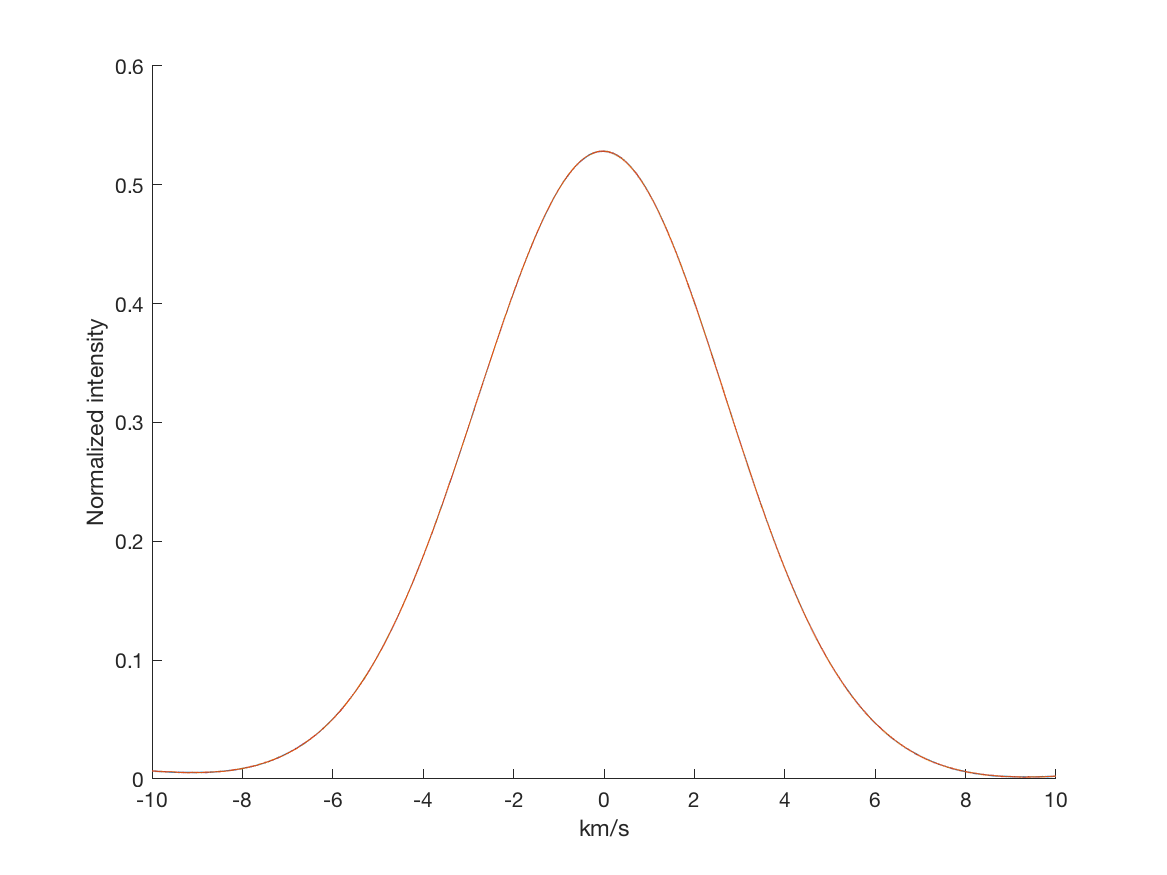
\includegraphics[width=\textwidth]{./Figures/Methods/LPD1-Line_Profile.png}
        \caption{Line profile (stacked)}
    \end{subfigure}
	~
    \begin{subfigure}[b]{0.49\textwidth}
        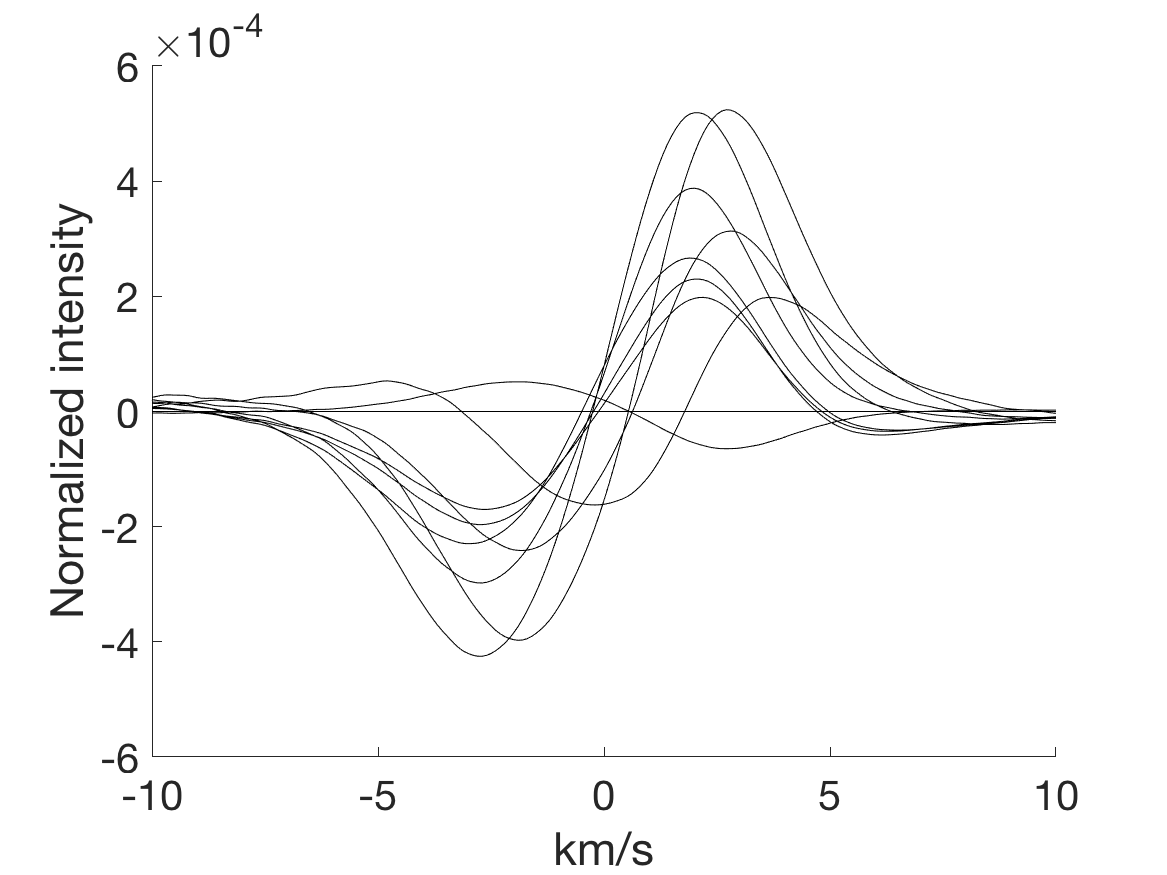
\includegraphics[width=\textwidth]{./Figures/Methods/LPD1-Differential_line_Profile.png}
        \caption{Differential line profile}
        \label{fig:ld_dlp}
    \end{subfigure}	
    
    \caption[Deformed line profile]{Deformed line profile. For the sake of clarity, the differential line profiles are plotted noise-free and only 10 out of 100 profiles are presented.}
\label{fig:line_profiles_deformation}
\end{figure}	
%-------------
\FloatBarrier

%----------------------------------------------------------------------------------------	
\subsection{Fourier phase spectrum analysis}

\subsubsection{$RV_\text{FT}$}
We took the same approach as previously (\S~\ref{ch:FT_line_shift}) to obtain the power spectrum and the differential phase spectrum (Fig.~\ref{fig:FT_process_LPD}) and measured radial velocities $RV_\text{FT}$ for the full range of frequencies. It is immediately apparent that a line deformation contributes to a skewed differential phase spectrum. As mentioned above, the shift $x_0(\xi)$ becomes frequency dependent, and is proportional to the local gradient of the differential phase spectrum. 

%-------------
\begin{figure}[tbp]	
    \begin{subfigure}[b]{0.49\textwidth}
        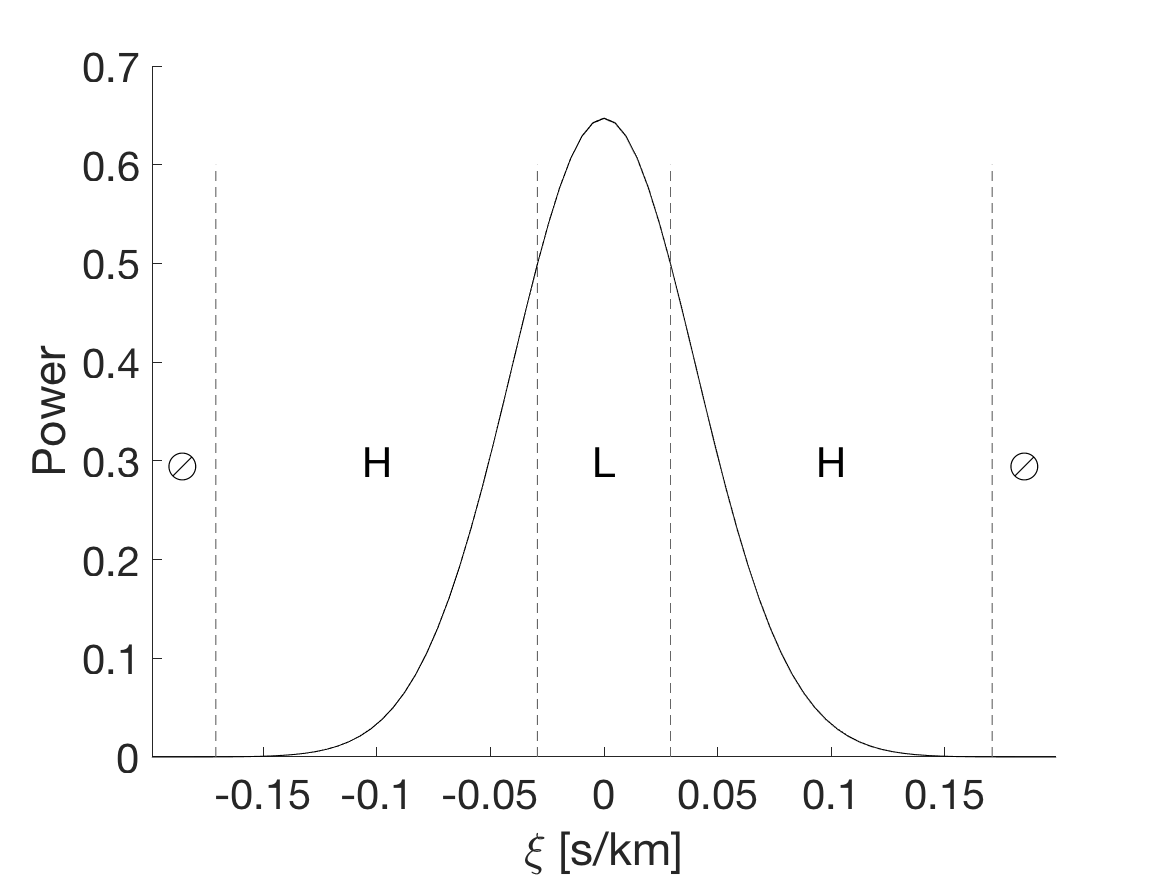
\includegraphics[width=\textwidth]{./Figures/Methods/LPD2-FT_power.png}
        \caption{Power spectrum (stacked)}
    \end{subfigure}
	~
    \begin{subfigure}[b]{0.49\textwidth}
        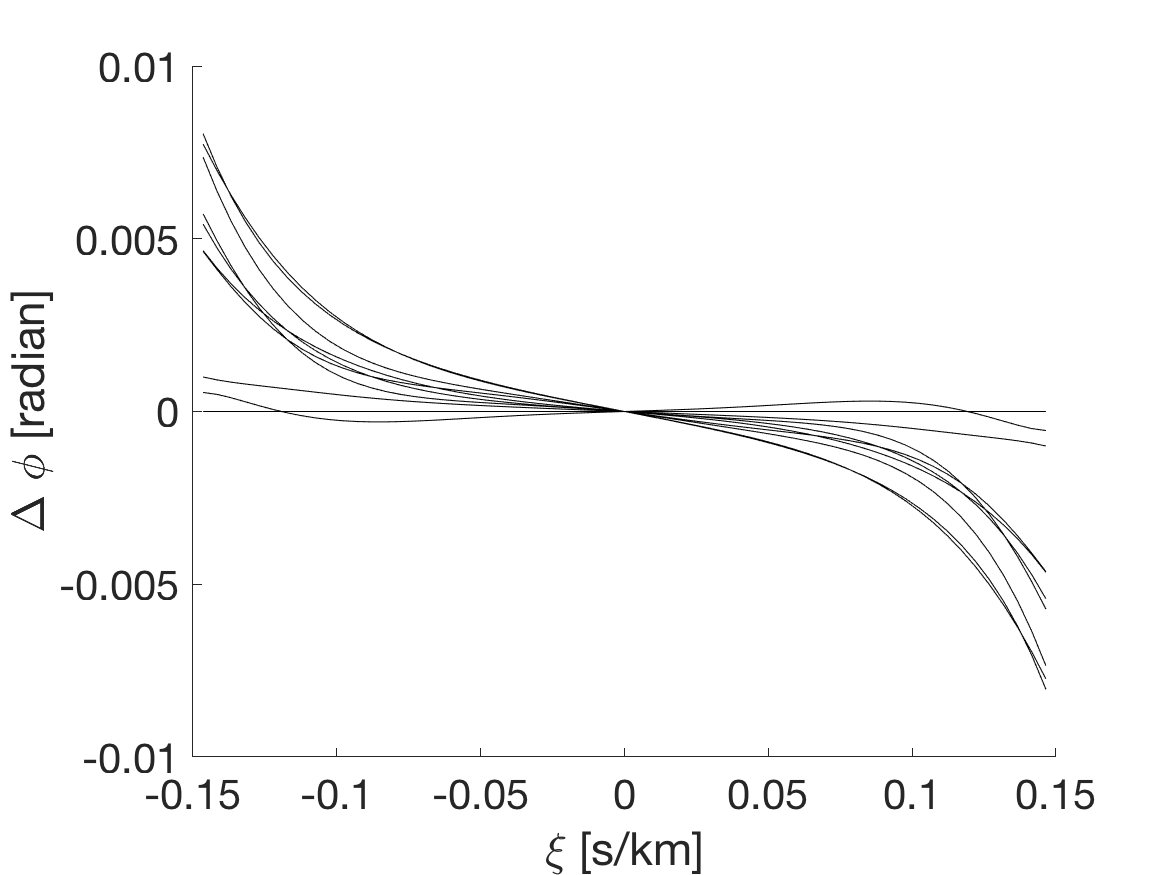
\includegraphics[width=\textwidth]{./Figures/Methods/LPD4-Relative_phase_angle.png}
        \caption{Differential phase spectrum}
        \label{fig:dps_LPD}
    \end{subfigure}
    
    \caption[Fourier transform of deformed line profiles]
    {Fourier transform of deformed line profiles. Only 10 out of 100 differential phase spectra are presented.}
\label{fig:FT_process_LPD}
\end{figure}    
%-------------

For deformed line profiles, the traditionally measured radial velocities would be solely the apparent radial velocities due to deformed line profiles (a.k.a. jitter). Both velocities $RV_\text{FT}$ and $RV_\text{Gaussian}$ are plotted against rotation phase (Fig.~\ref{fig:rv_recovery_deformed}). If we take $\sigma_\text{FT} = \sigma_\text{Gaussian} = 0.08$ m/s to be the intrinsic photon noise level corresponding to S/N = 10,000 as measured in \S~\ref{sec:Initial_tests}, and assume $RV_\text{FT}$ and $RV_\text{Gaussian}$ are independent measurements, the difference between $RV_\text{FT}$ and $RV_\text{Gaussian}$ would have an uncertainty of $\sqrt{\sigma_\text{FT}^2+\sigma_\text{Gaussian}^2}\approx0.11$ m/s. Fig.~\ref{fig:rv_recovery_deformed} presents $\mid \Delta RV \mid = \mid RV_\text{FT} - RV_\text{Gaussian}\mid < 0.01$ m/s. Therefore, we can see that $RV_\text{FT}$ and $RV_\text{Gaussian}$ are indistinguishably consistent in the measurement of the apparent radial velocities of a deformed line profile. There is, however, a very small amount of bias between these two methods, as seen in the $\Delta RV$ trend. Increasing the cut-off frequency wisely can mitigate such bias. 

%-------------
\begin{figure}[tbp]
\centering
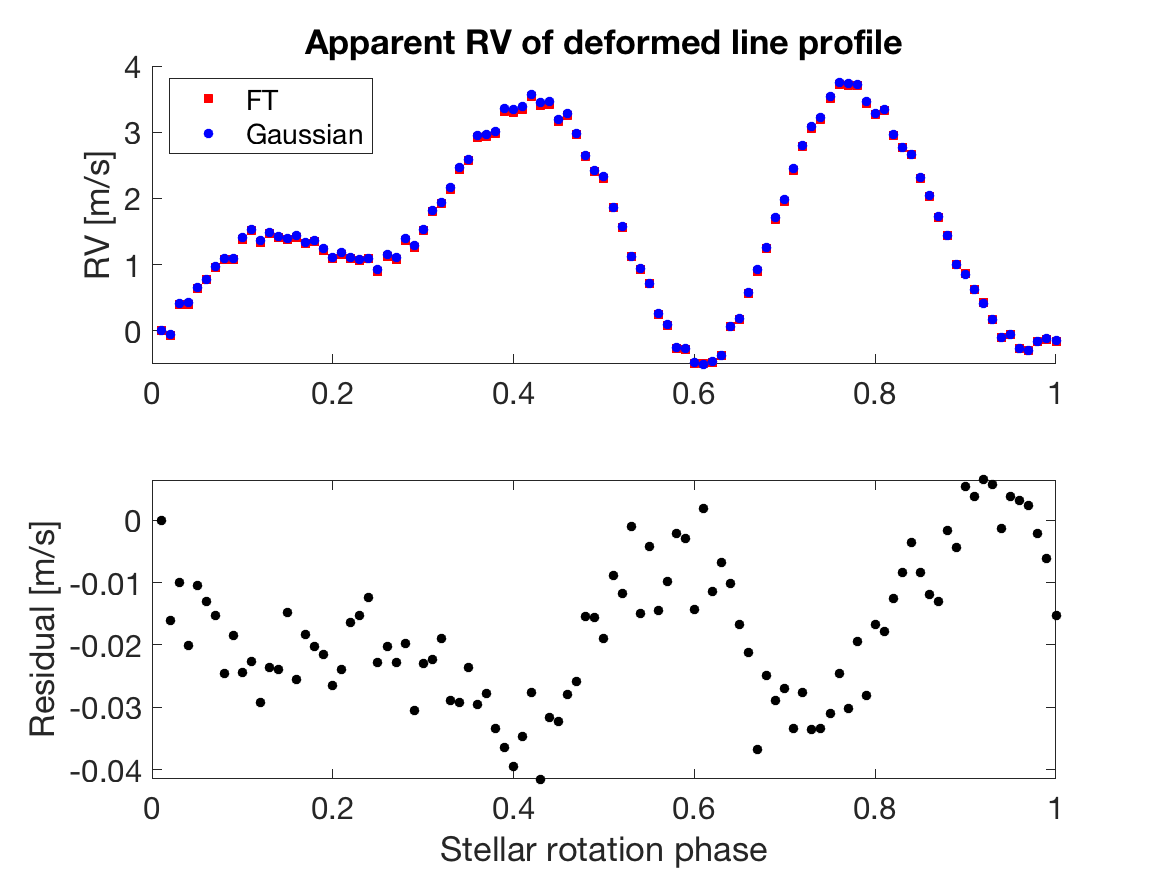
\includegraphics[width = 0.7 \linewidth]
{./Figures/Methods/5-JITTER_ONLY_3.png}
\caption[Apparent RV of deformed line profiles]
{Apparent RV of deformed line profiles calculated with both $\mathit{\Phi}$ESTA and Gaussian fit to the line profile. Both results are also highly consistent with each other. $\Delta RV  = RV_\text{FT} - RV_\text{Gaussian}$.}
\label{fig:rv_recovery_deformed}
\end{figure} 
%-------------
\FloatBarrier

%----------------------------------------------------------------------------------------	
\subsubsection{$RV_\text{FT,H}$ and $RV_\text{FT,L}$}
\label{subsec:FT,HL}

Although an intrinsic line deformation (in the absence of any velocity shift in the host star) usually mimics a radial velocity shift, we note the shape differences in the differential phase spectrum between an actual line shift (Fig.~\ref{fig:dps}) and a line deformation (Fig.~\ref{fig:dps_LPD}) -- the latter presents slightly flatter features in lower frequencies and becomes more skewed towards higher frequencies. Such differences provide key information for differentiating the two situations.

According to \S\ref{sec:LD_Theory} where we introduced $\overline{x_0(\xi)}$ -- an averaged shift for a particular frequency range -- we compute the equivalent radial velocity shift for each of the lower and higher frequency ranges. We present our results by plotting the obtained $RV_\text{FT,H/L}$ against the jitter (line centroid fitted by a Gaussian profile) in Fig.~\ref{fig:FT_vs_Gaussian}. The $RV_\text{FT,H}$ and $RV_\text{FT,L}$ are both linearly correlated with the jitter though with different slopes. Fitting with a linear regression model, it comes with a slope $k_\text{H} = 1.491\pm0.053~(\pm3.5\%)$ for $RV_\text{FT,H}$, meaning an apparent radial velocity shift of 1 m/s due to line deformation is detected as a $1.491\pm0.053$ m/s shift on average using \textit{this} high-pass filter; whereas the slope for applying a low-pass filter is $k_\text{L} = 0.750\pm0.027~(\pm3.6\%)$, not as ``responsive" as $RV_\text{FT,H}$ to the line profile deformation. It's also worth (and interesting) noting that the combined effect of these two filters would have resulted in $RV_\text{FT}$, a consistent measurement of the radial velocity as with the fitting a line centroid as previously showed.

%-------------
\begin{figure}[tbp]
\centering
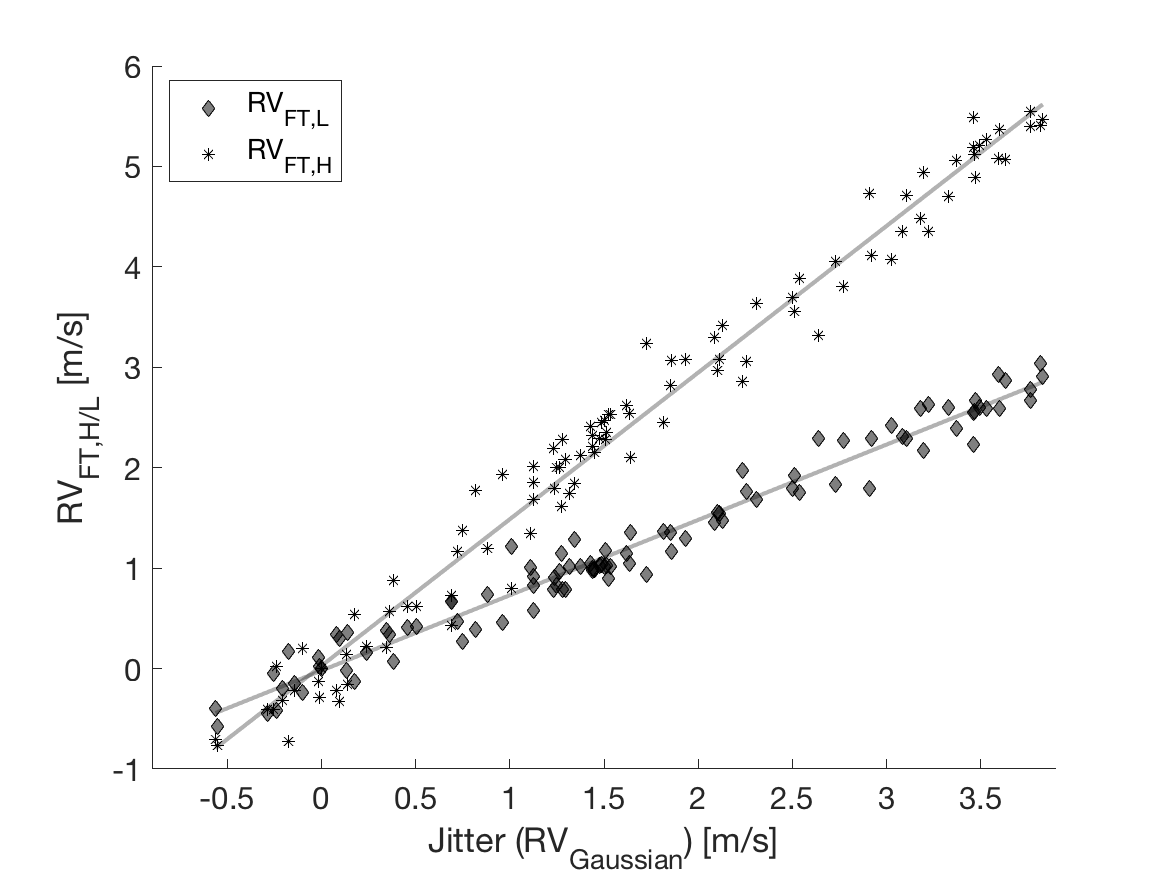
\includegraphics[width = 0.7 \linewidth]
{./Figures/Methods/5-JITTER_ONLY_1.png}
\caption[Fourier transform in response to line deformation]
{Applying the low-pass and high-pass filters, the Fourier transform $RV_\text{FT,L}$ and $RV_\text{FT,H}$ are linearly correlated with the jitter ($RV_\text{Gaussian}$).}
\label{fig:FT_vs_Gaussian}
\end{figure} 
%-------------

We can investigate how well this correlation behaves for each filter by scaling the measured $RV_\text{FT,L}$ and $RV_\text{FT,H}$ by their corresponding factors $1/k_\text{L}$ and $1/k_\text{H}$ respectively, and compare them with the jitter ($RV_\text{Gaussian}$), presented in Fig.~\ref{fig:scaling_RV_FT}. The standard deviations for the residuals are $\sigma_\text{FT,H} \approx 0.18$ m/s and $\sigma_\text{FT,L} \approx 0.22$ m/s respectively, offering similar performance.

%The reason for $\sigma_\text{FT,H}>\sigma_\text{FT,L}$ is the same as mentioned in \S\ref{sec:Further_tests} -- higher frequency modes are more sensitive to noise, but the fact that both $\sigma_\text{FT,H/L}$ increase (opposed to $\sigma_\text{FT,H/L}$ = 0.08~m/s in the case of a pure line shift) is because we think the linearity between $RV_\text{FT,H/L}$ and the input jitter is only empirically valid but not strictly followed. The deviation from linearity would affect how well we could recover the jitter by scaling $RV_\text{FT,H/L}$ and may also introduce systematics in the recovery of jitter. 

%-------------
\begin{figure}[tbp]
\centering
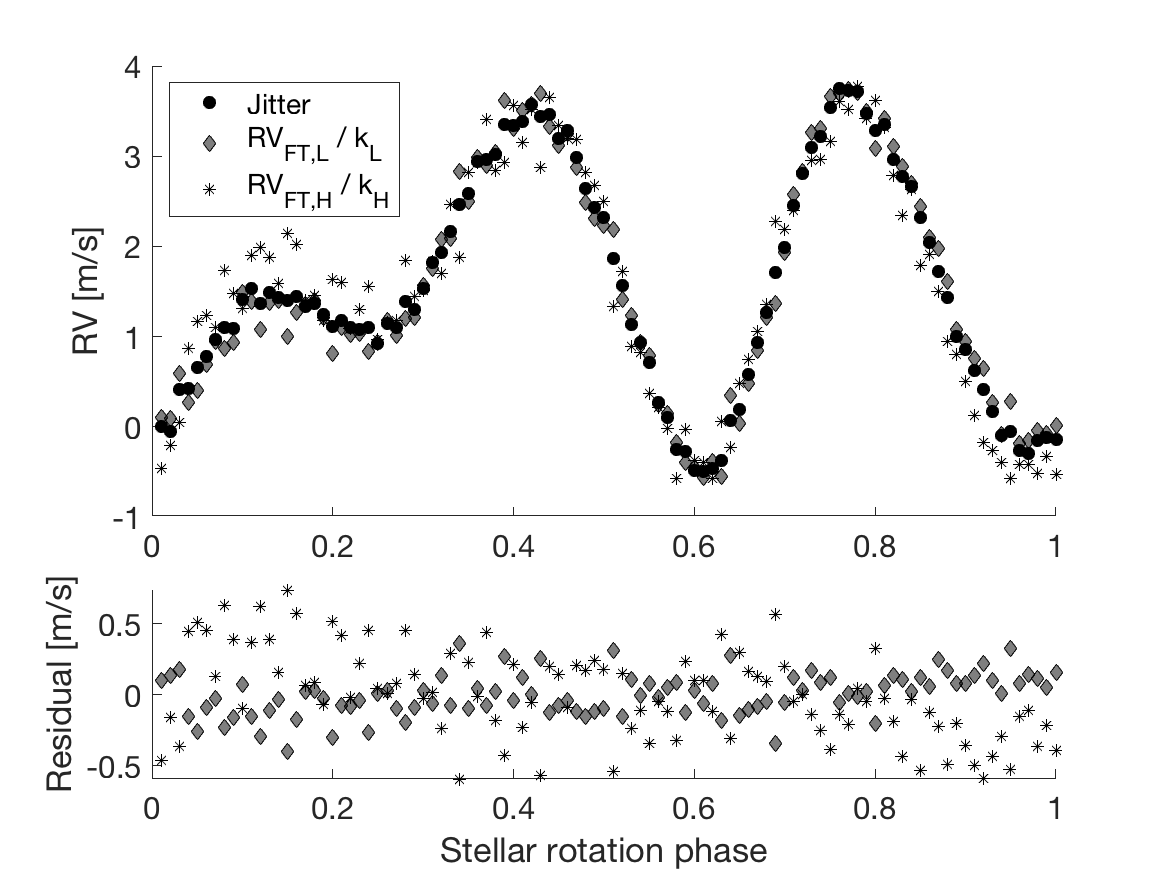
\includegraphics[width = 0.7 \linewidth]
{./Figures/Methods/5-JITTER_ONLY_4.png}
\caption[Scaling the low-pass and high-pass Fourier transformed radial velocities]
{Scaling the low-pass and high-pass Fourier transformed radial velocities to match the input jitter.}
\label{fig:scaling_RV_FT}
\end{figure} 
%-------------

%----------------------------------------------------------------------------------------	
\subsection{Jitter model}
\label{subsec:Jitter_model}

We have shown in \S~\ref{ch:FT_line_shift} that the following measurable quantities demonstrate essentially the same response to pure line shifts: $RV_\text{FT}$, $RV_\text{FT,H}$, $RV_\text{FT,L}$ and $RV_\text{Gaussian}$. We have also shown in \S~\ref{sec:FT_ld} that both $RV_\text{FT,H}$ and $RV_\text{FT,L}$ are linearly correlated with the jitter, and $RV_\text{FT,H}$ is more responsive ($k_\text{H}>1$) than $RV_\text{FT,L}$ ($k_\text{L}<1$). 

We can therefore write the following measurable quantities -- $RV_\text{Gaussian}$ (or $RV_\text{FT}$), $RV_\text{FT,L}$ and $RV_\text{FT,H}$ -- in the from of three additive terms: (1) a bulk shift in the star (which we hereafter assume to be due to a planet or planets as the superposition of Keplerian orbit(s)), (2) variability in the stellar line profile (hereafter lumped under the general name ``jitter''), and (3) a constant radial velocity offset term chosen so as to be absorbed into the previous two terms.
\begin{align}
	RV_\text{Gaussian} 	&= RV_\text{planet} + RV_\text{jitter}				 \label{eq:RV_Gau} \\
	RV_\text{FT,L} 		&= RV_\text{planet} + k_L \cdot RV_\text{jitter} 		 \label{eq:RV_FTL} \\
	RV_\text{FT,H} 		&= RV_\text{planet} + k_H \cdot RV_\text{jitter}.		 \label{eq:RV_FTH}
\end{align}
Subtracting these equations to remove $RV_\text{planet}$, we reduce to two independent equations
\begin{align}
	RV_\text{Gaussian} - RV_\text{FT,L} 	&= (1-k_L) \cdot RV_\text{jitter}\\
	RV_\text{FT,H} - RV_\text{Gaussian}	&= (k_H-1) \cdot RV_\text{jitter}
\end{align}
Rearranging yields two expressions for the jitter model
\begin{align}
	RV_\text{jitter} &= \frac{RV_\text{Gaussian} - RV_\text{FT,L}}{1-k_L} 	\label{eq:jitter_model1} \\
	RV_\text{jitter} &= \frac{RV_\text{FT,H} - RV_\text{Gaussian}}{k_H-1}		\label{eq:jitter_model2} 
\end{align}
where $RV_\text{Gaussian}, RV_\text{FT,L}$ and $RV_\text{FT,H}$ are direct measurements, whereas $k_L$ and $k_H$ are unknowns. We could determine $k_L$ and $k_H$ in the previous simulations only because we knew there were no radial velocities, other than jitter, in the system. These two expressions for the jitter model will be frequently used throughout the rest of the chapter. We therefore simplify $(RV_\text{Gaussian} - RV_\text{FT,L})$ as $\Delta RV_\text{L}$ and $(RV_\text{FT,H} - RV_\text{Gaussian})$ as $\Delta RV_\text{H}$ and call them the jitter metrics. Dividing the two equations above further cancels $RV_\text{jitter}$ to give
\begin{equation}
	\frac{\Delta RV_\text{H}}{\Delta RV_\text{L}} = \frac{k_H-1}{1-k_L} \triangleq k_{H/L}.
\label{eq:GHL} 
\end{equation}
This means $(1-k_H)/(1-k_L)$ can now be obtained by fitting a linear regression model for $\Delta RV_\text{H}$ against $\Delta RV_\text{L}$. With this, we rewrite the jitter model in a unified form -- the weighted sum of the two jitter expressions from Eq.~\ref{eq:jitter_model1} and Eq.~\ref{eq:jitter_model2}: 
\begin{align*}
	RV_\text{jitter} &= w_1 \frac{\Delta RV_\text{L}}{1-k_L} + w_2 \frac{\Delta RV_\text{H}}{k_H-1} \\
	&= \frac{1}{{1-k_L}} \bigg(w_1 \Delta RV_\text{L} + w_2 \frac{\Delta RV_\text{H}}{\frac{k_H-1}{1-k_L}} \bigg) \\
	&= \alpha \bigg(w_1 \Delta RV_\text{L} + w_2 \frac{\Delta RV_\text{H}}{k_{H/L}} \bigg) \numberthis \label{eq:jitter_model_final}
\end{align*}
in which the weights satisfy $w_1+w_2=1$ and $1/(1-k_L)$ is replaced by the scaling factor $\alpha$. 

%Additionally, we can roughly estimate the uncertainty of $RV_\text{jitter}$ in Eq.~\ref{eq:jitter_model1} and Eq.~\ref{eq:jitter_model2} by treating $RV_\text{Gaussian}$, $RV_\text{FT,L}$ and $RV_\text{FT,H}$ are independent variables, and $k_{L/H}$ is a constant: 
%\begin{align}
%	\Delta RV_\text{jitter,L} &\approx \frac{\sqrt{\sigma_\text{Gaussian}^2 + \sigma_\text{FT,L}^2}}{1-k_L} \\
%	\Delta RV_\text{jitter,H} &\approx \frac{\sqrt{\sigma_\text{Gaussian}^2 + \sigma_\text{FT,H}^2}}{k_H-1}.
%\end{align}
%Substituting the following values: $\sigma_\text{Gaussian} = 0.08$ m/s (\S\ref{sec:Initial_tests}), $\sigma_\text{FT,L} = 0.11$ m/s and $\sigma_\text{FT,H} = 0.43$ m/s (\S\ref{sec:Further_tests}), $k_L = 0.847$ and $k_H = 1.978$ (\S\ref{subsec:FT,HL}), we obtain $\Delta RV_\text{jitter,L} = 0.89$ m/s and $\Delta RV_\text{jitter,H} = 0.45$ m/s.

An obvious check is to examine the correlation between $\Delta RV_\text{H}$ and $\Delta RV_\text{L}$ (Eq.~\ref{eq:GHL}) before going ahead creating the jitter model (Eq.~\ref{eq:jitter_model1} and Eq.~\ref{eq:jitter_model2}). As our jitter model is solely based on the empirically assumed linear correlations between $RV_\text{FT,H}$, $RV_\text{FT,L}$ and $RV_\text{jitter}$, if either of these correlations fails, this can be detected by plotting $\Delta RV_\text{H}$ against $\Delta RV_\text{L}$.

%----------------------------------------------------------------------------------------	
\subsection{Testing the recovery of jitter}
\label{sec:check}

To begin with, we introduce a technique that smooths over noise in the observed signals -- \textbf{weighted moving average} modulated by a Gaussian kernel. For $N$ data points (e.g. radial velocities) $v_i$ with an uncertainty $\sigma_i$ observed at $t_i$ ($i=1,2,...N$), we define the contribution (i.e. weight) of a data point $(t_i, v_i\pm \sigma_i)$ towards the chosen position $t$ as the multiplication of two factors: (1) the weight of the data point itself, inversely proportional to the uncertainty squared: $W_i= 1/{\sigma_i^2}$ and (2) a stationary kernel that describes the correlation between data, depending on their distance $\mid t-t_i \mid$ and a time-scale of correlation $\tau$: $K_i(t) = e^{-\frac{(t-t_i)^2}{2\tau^2}}$. With this, the evaluation of a data point $v(t)$ can be drawn by the weighted average of all observed data $(t_i, v_i\pm \sigma_i)$, with the weight 
\begin{equation}
	\textbf{W}_i(t) = W_i \cdot K_i(t) = \frac{1}{\sigma_i^2} e^{-\frac{(t-t_i)^2}{2\tau^2}}
\end{equation}
respectively and then normalised by the sum of weights, so that 
\begin{equation}
	v(t) 	=  \frac{\sum\limits_{i=1}^{N} \bigg[v_i*\textbf{W}_i(t)\bigg]}{\sum\limits_{i=1}^{N} \textbf{W}_i(t)}
\end{equation}


To perform tests of the recovery of artificially generated jitter using Eq.~\ref{eq:jitter_model_final}, we doubled the amount of line profiles in the form of cross-correlation functions (i.e. simulated over a time equivalent to two stellar rotations), and each line profile is further shifted by an amount $RV_\text{planet}$ with an amplitude of the Keplerian orbit $A_\text{planet} = 2~\text{m/s}$ (although in principle the $RV_\text{planet}$ configuration shouldn't affect the jitter model because the term was cancelled out when we derived the jitter expression). In the simulation, the stellar rotation period is a known quantity. To generally address the planetary orbital period, we talk about the ratio relative to one stellar rotation. For example, the planetary orbital frequency to stellar rotation frequency ratio is set to be 0.7 (i.e. $\nu_\text{orb}/\nu_\text{rot} = P_\text{rot}/P_\text{orb} = 0.7$). 

We then obtained three sets of radial velocities for each simulated profile: $RV_\text{Gaussian}$, $RV_\text{FT,H}$ and $RV_\text{FT,L}$ (Fig.~\ref{fig:PLANET_AND_JITTER} upper panel). We tested three different combinations of $w_1$ and $w_2$ in Eq.~\ref{eq:jitter_model_final}: (1) $w_1=1, w_2=0$; (2) $w_1=0.5, w_2=0.5$; (3) $w_1=0, w_2=1$, each is multiplied by their respective scaling factor (fitted by linear regression to the known input jitter) to see how well it matches the input jitter. The middle panel demonstrates a consistent recovery of jitter among the three expressions of jitter model, albeit with small differences. A weighted moving average was applied to show the trend. The lower panel is the residual of the fitting, with the weighted moving average on top. 

%-------------
\begin{figure}[tbp]
\centering
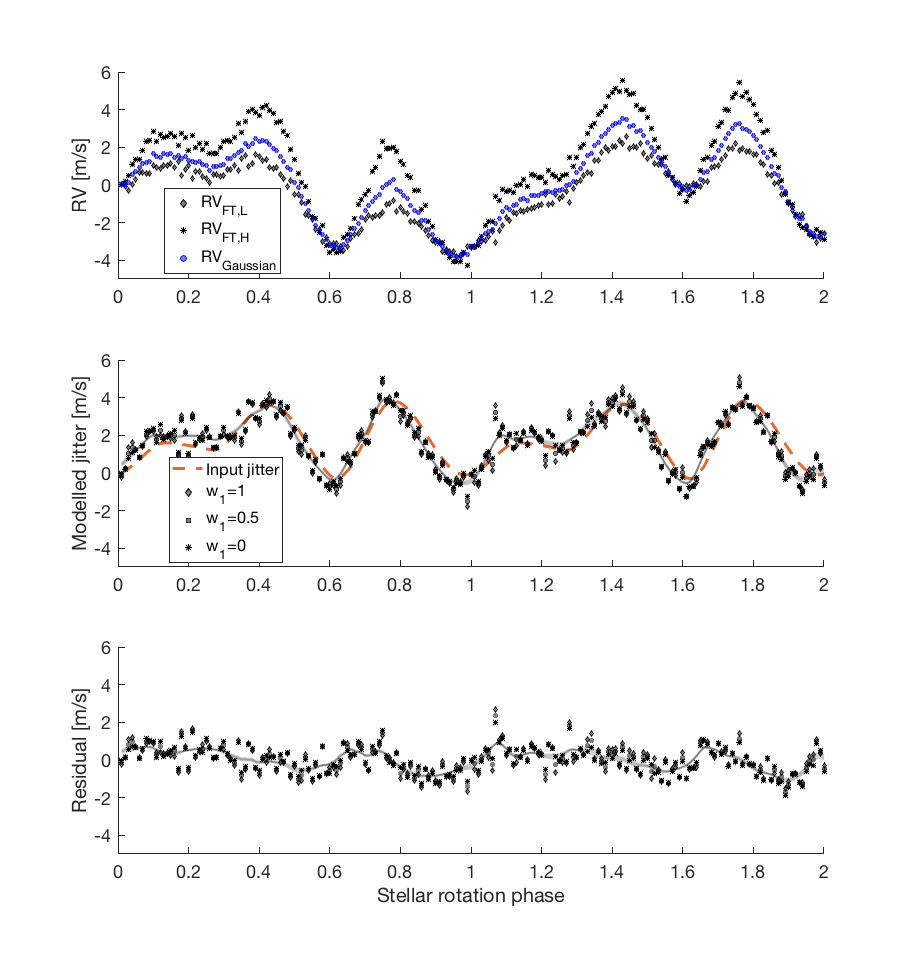
\includegraphics[width = 0.99 \linewidth]
{./Figures/Methods/5-PLANET_AND_JITTER2.png}
\caption[Jitter model]
{Jitter recovery based on Eq.~\ref{eq:jitter_model_final} for simulated data with S/N = 10,000. Top: time series of directly measured $RV_\text{Gaussian}$, $RV_\text{FT,L}$ and $RV_\text{FT,H}$. Middle: three forms of jitter $(w_1 = 1, 0.5$ and 0) scaled to match the input jitter, and smoothed by the weighted moving average (grey solid lines) with $\tau$ equal to the spacing of two samplings to show the trend of the recovered jitter. For comparison, the input jitter is labelled as the orange dashed line. Bottom: difference between the jitter model and the input jitter, smoothed by the weighted moving average (grey solid lines). Differences between the three expressions for jitter are small (...). Note the scaling across the three subplots are the same.}
\label{fig:PLANET_AND_JITTER}
\end{figure} 
%-------------

To quantitatively examine the performance of the jitter models, we compare the scatter of data before and after the jitter model is applied (i.e. middle and bottom panels of Fig.~\ref{fig:PLANET_AND_JITTER}). The scatter due to jitter is $\sigma_\text{jitter} = 1.22$~m/s (orange dashed line in the middle panel), and the scatter of residuals can be found in Table~\ref{table:jitter_model_scatter}, mainly depending on the S/N and whether and how smoothing is adopted. In addition to the high S/N (=~10,000) simulations \footnote{This is the typical S/N found in the cross-correlation line profiles of HARPS observations of $\alpha$ Cen B.}, we also simulate a moderate noise condition: S/N = 2,000 \footnote{S/N ranging from 2,000 to 4,000 are found in a dwarf star HD~189733 with apparent magnitude $V=7.6$; lower S/N$\sim$1,000 are found for red dwarfs Gl~176 and Wolf~1061 with $V\sim10$.}.

%-------------
\begin{table}[htbp]
\centering
\begin{tabular}{|c|c|c|c|c|}
\hline
\multirow{2}{*}{} 	& \multicolumn{2}{c|}{$\sigma_\text{residual}$ (raw) [m/s]}  & \multicolumn{2}{c|}{$\sigma_\text{residual}$ (smoothed) [m/s]}  \\ \cline{2-5} 
                  	& \multicolumn{1}{l|}{S/N=10,000} & \multicolumn{1}{l|}{S/N=2,000} & \multicolumn{1}{l|}{S/N=10,000} & \multicolumn{1}{l|}{S/N=2,000} \\ \hline
$w_1=1, w_2=0$  	 	& 0.72 		& 2.51 			& 0.46 			& 0.74                              \\ \hline
$w_1=0.5, w_2=0.5$  & 0.69 		& 2.07			& 0.51			& 0.64                              \\ \hline
$w_1=0, w_2=1$      & 0.69		& 2.20			& 0.48 			& 0.68                              \\ \hline
\end{tabular}
\caption{Residuals after applying our jitter model (in comparison with $\sigma_\text{jitter} = 1.22$~m/s)}
\label{table:jitter_model_scatter}
\end{table}
%-------------

We note from the table, that the scatter due to the simulated jitter is reduced from $\sigma_\text{jitter} = 1.22$~m/s to $\sigma_\text{residual} \sim 0.70$~m/s for S/N=10,000, but increased to 2.0~-~2.5~m/s for S/N=2,000. Implementing the weighted moving average with a meaningful correlation time-scale $\tau$ can further reduce $\sigma_\text{residual}$. In this exercise, we choose the time-scale for S/N=10,000 to be twice the spacing between two subsequent simulated observations, and for S/N=2,000 5 times the spacing. We also tested other smoothing approaches, such as the Python \verb|PyMC3| implementation of Gaussian process smoothing, with similar results. 

We note that after jitter correction, the residuals $\sigma_\text{residual}$ are still larger than that from simulations without planets (\S~\ref{sec:Simulations}). This is not because the presence of a planet alters the residuals, but rather die to the different ways in which jitter was dealt with. In \S~\ref{sec:Simulations}, we know our simulations have no planets, so that the measured $RV_\text{FT,H}$ and $RV_\text{FT,L}$ are solely proportional to the input jitter (scaling factor $\sim 0.7$ and $\sim 1.3$ respectively). In reality, we have no idea if there are planets in the system, so to construct the jitter model is first to remove the contributions from planets (E.q.~\ref{eq:jitter_model1} and \ref{eq:jitter_model2}). Doing so requires scaling $\Delta RV_\text{H}$ and $\Delta RV_\text{L}$ by a factor of 2~-~4, and thus increasing the scatter of residuals. 

In conclusion, we have demonstrated sub-m/s results for the residuals after implementing a jitter correction derived from $\mathit{\Phi}$ESTA. This indicates the potential to enhance the detection of planets at sub-m/s precisions and reveal candidates with radial velocities of sub-m/s amplitudes in the presence of stellar variability. However, this does require good data sampling and moderate-to-high S/N data. 

% we should not ignore there can be systematic differences between the actual jitter and our jitter models.

%----------------------------------------------------------------------------------------
\subsection{Planetary radial velocity recovery}

Having obtained the jitter model (Eq.~\ref{eq:jitter_model_final}) and assuming $RV_\text{planet}$ follows a Keplerian orbital motion, we can turn our planetary radial velocity recovery into a model fitting problem, in which the parameters of the jitter model (such as the scaling factor) and that of the Keplerian orbit (such as amplitude, orbital period and phase) need to be determined. 

Alternatively, we can bypass the jitter model. Revisiting the Equations \ref{eq:RV_Gau}-\ref{eq:RV_FTH}, we rewrite them by observation number $i (i=1,2,\ldots,N)$ and switch the notation to obtain the following $3N$ independent linear equations:
\begin{align}
	X_i 		&= P_i + J_i				\label{eq:XX} \\
	Y_i 		&= P_i + k_y \cdot J_i	\label{eq:YY} \\
	Z_i 		&= P_i + k_z \cdot J_i 	\label{eq:ZZ}
\end{align}
where $X_i, Y_i$ and $Z_i$ replace the three measurable radial velocities $RV_\text{Gaussian}$, $RV_\text{FT,L}$ and $RV_\text{FT,H}$; $P_i$ and $J_i$ are the planetary and the jitter radial velocities; and $k_y$ and $k_z$ are the scaling factors $k_L$ and $k_H$. Substituting $J_i = X_i - P_i$ from Eq.~\ref{eq:XX}, we can simplify the system to $2N$ independent linear equations:
\begin{align}
	Y_i 		&= k_y \cdot X_i + (1-k_y)P_i	\label{eq:YYY} \\
	Z_i 		&= k_z \cdot X_i + (1-k_z)P_i	\label{eq:ZZZ}.
\end{align}
The number of unknowns is $(N+4)$, including $N$ from $P_i$, 2 from $k_y$ and $k_z$, and another 2 from the previously absorbed constant offsets. Normally we have $N \gg 1$, so that the number of independent equations ($2N$) is larger than the number of degrees of freedom $(N+4)$ in the system, meaning the system can be uniquely solved by optimization, such as least square minimization of the objective function:
\begin{equation}
	\sum_{i=1}^{N} \Bigg[w_{y,i}\Big(k_y \cdot X_i + (1-k_y)P_i - Y_i \Big)^2 + w_{z,i}\Big(k_z \cdot X_i + (1-k_z)P_i- Z_i \Big)^2 \Bigg]
\label{eq:objective_function}
\end{equation}
where $w_{y,i}$ and $w_{z,i}$ are pre-determined weights (e.g. determined by the sizes of errorbars of the observed radial velocities). Due to the intricacy of involving $(N+4)$ unknowns in the minimization, we have not yet managed to solve this problem in a timely manner, but it is worth investigating in the future, as it can return a best fit solution for $P_i$, from which we can further derive the planetary signals. 

%This approach becomes identical to constructing a jitter model (Eq.~\ref{eq:jitter_model_final}) in cases where (1) $w_{y,i}=1, w_{z,i}=0 (i=1,2,\ldots,N)$ and $w_1=1, w_2=0$; (2) $w_{y,i}=0, w_{z,i}=1 (i=1,2,\ldots,N)$ and $w_1=0, w_2=1$.

\subsection{Conclusion}

Fourier phase spectrum analysis ($\mathit{\Phi}$ESTA or FIESTA) can be used to combine information from the power and phase spectra to return radial velocities consistent with those acquired by fitting a Gaussian function to a line profile. This conclusion applies both for measuring a direct line shift and an apparent shift of a deformed line profile. 

The frequency dependent $x_0(\xi)$ is the key asset in identifying line profile deformation and distinguishing it from a bulk line shift. We have investigated the apparent radial velocity shift (i.e. jitter) produced by deformed line profiles and shown it can be considered as the combination of two radial velocities -- $RV_\text{FT,H}$ in higher frequency modes and $RV_\text{FT,L}$ in lower frequency modes. They both correlate linearly with jitter (as obtained from the simulated spectral line profiles). 

The different strengths of these correlations for $RV_\text{FT,H}$ and $RV_\text{FT,L}$ enable us to calculate the jitter metrics and construct a jitter model, which can recover simulated radial velocities data when in the presence of stellar variability, in both high-and-moderate S/N simulations. 

\pagebreak
%----------------------------------------------------------------------------------------	
%----------------------------------------------------------------------------------------	
\section{End-to-end simulations}
\label{\thesection}
\label{sec:end-to-end}

We ran end-to-end simulations to test the performance of $\mathit{\Phi}$ESTA for recovering a planetary signal in the presence of jitter. Specifically, we sought to answer the following three questions:
\begin{enumerate}
	\item When the amplitude of jitter is comparable to that of planetary radial velocities, can we better recover the planet orbital parameters with $\mathit{\Phi}$ESTA? 
	\item When planetary radial velocities dominate and jitter is negligible, does $\mathit{\Phi}$ESTA give at least equally good results as traditional methods (i.e. without jitter correction)? 
	\item When jitter is the only source of radial velocity variation, can it be identified with the help of $\mathit{\Phi}$ESTA?
\end{enumerate}

In the following simulations, the spectral line profile simulator (SOAP 2.0) is used as the same manner as previously. We adjust the planetary orbital amplitude with respect to a $\sim 2$~m/s jitter amplitude to satisfy the three categories above. For S/N, we choose two numbers to represent in the simulations: (1) S/N = 10,000 where we examine $\mathit{\Phi}$ESTA for the detection of planets orbiting bright and active stars; and (2) S/N = 2,000 where noise in the data pushes the limit of $\mathit{\Phi}$ESTA's usefulness. We ran 500 trials, each trial with 60 randomly selected samples clustered in 12 groups, out of a total of 400 equally spaced samples from four stellar rotations (Fig.~\ref{fig:Sampling_demo}). 

%-------------
\begin{figure}[hbp]
\centering
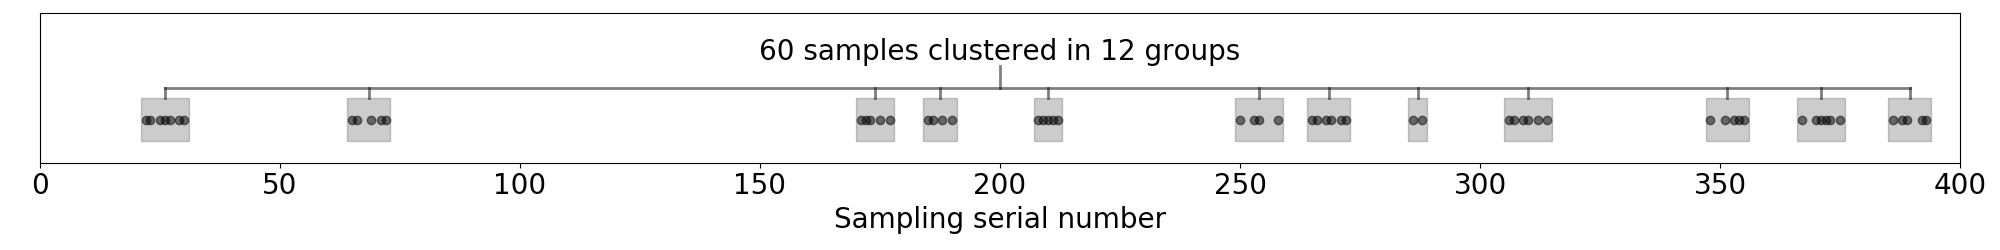
\includegraphics[width = 0.99 \linewidth]
{./Figures/Methods/Sampling_demo.png}
\caption[How sampling is made]
{Demonstration of how time sampling is made. Whist the sampling of each trial is randomized, we keep a total of 60 samplings within 12 groups.}
\label{fig:Sampling_demo}
\end{figure} 
%-------------

The tests are divided into two main groups for comparison:
\begin{enumerate}
	\item fit $RV_\text{Gaussian}$ by Keplerian orbit alone; and
	\item fit $RV_\text{Gaussian}$ by Keplerian orbit with jitter model correction. The following three variations of model fitting were tested:
   \begin{enumerate}
     \item Jitter model constructed with $RV_\text{Gaussian}$ and $RV_\text{FT,L}$ only, i.e. $w_1=1$ and $w_2=0$;
     \item Jitter model constructed with $RV_\text{Gaussian}$ and $RV_\text{FT,H}$ only, i.e. $w_1=0$ and $w_2=1$;
     \item Jitter model constructed with $RV_\text{Gaussian}$, $RV_\text{FT,L}$ and $RV_\text{FT,H}$, represented by $w_1=0.5$ and $w_2=0.5$ in our test. 
   \end{enumerate}
\end{enumerate}

The parameters for each fit were obtained by Markov chain Monte Carlo (MCMC) optimization of an object function that minimizes the differences between simulated radial velocities and the models mentioned above. Fig.~\ref{fig:Corner} shows an output of the MCMC samplings in the parameter space, composed of an orbital amplitude $A$, an orbital frequency $\nu$ (defined as the ratio over known stellar rotation frequency), an initial phase $\omega$, an offset $\beta$, and additional for the jitter model a scaling factor $\alpha$. All the radial velocity data were equally weighted, as they have the same S/N in each simulation. From each set of 3 fits in Group~2 we selected the one with the smallest residuals (i.e. smallest rms) as our preferred solution. 

%-------------
\begin{figure}[tbp]	
    \begin{subfigure}[b]{0.49\textwidth}
        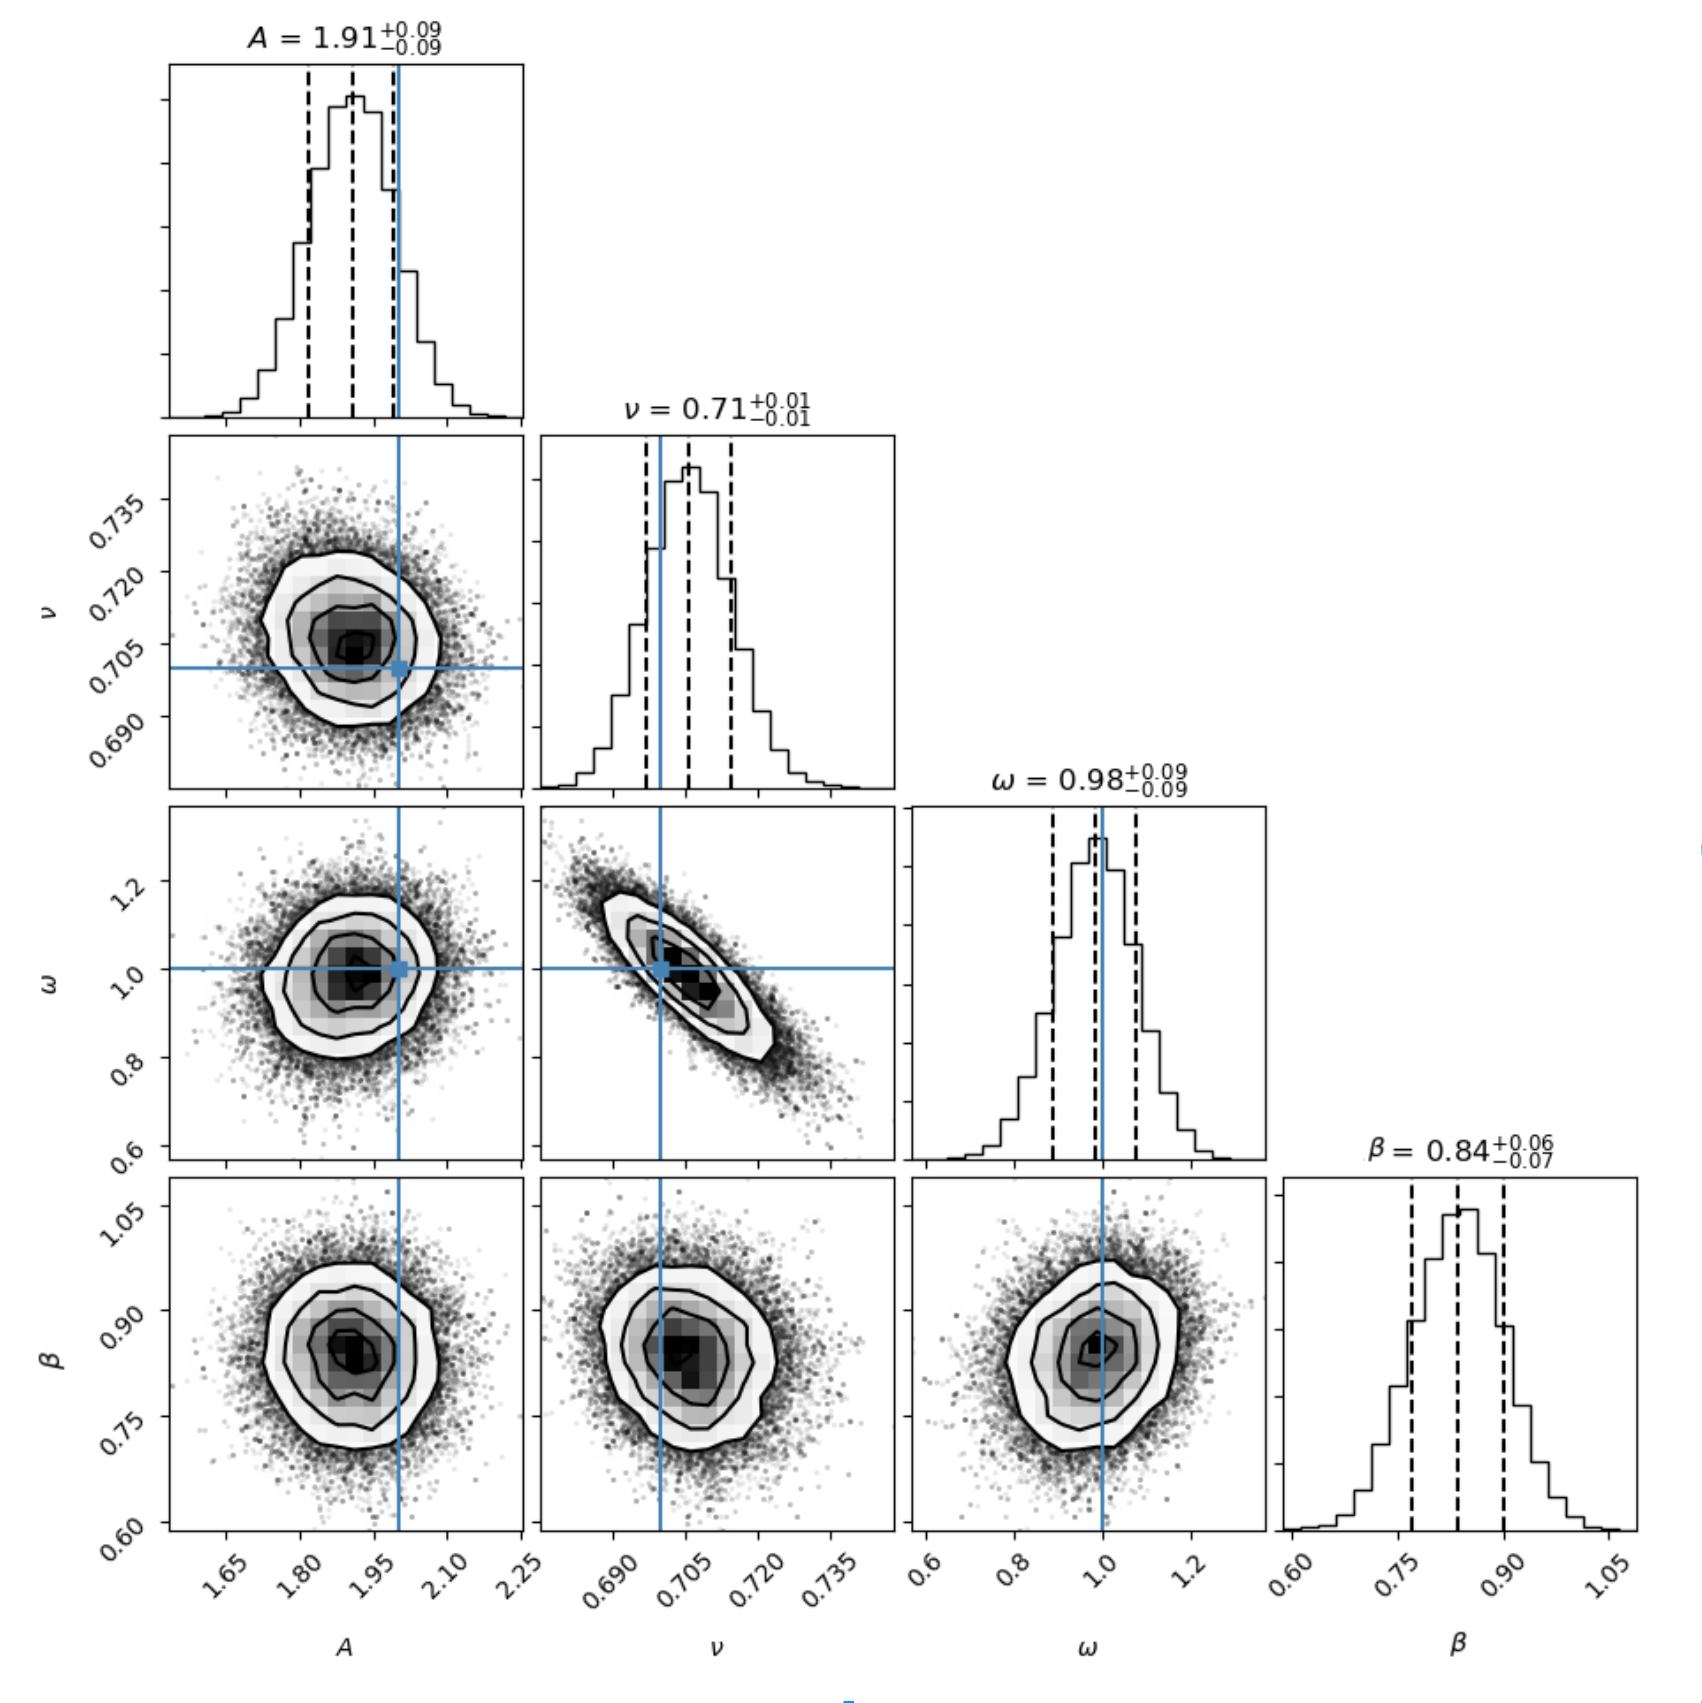
\includegraphics[width=\textwidth]{./Figures/Methods/Fitting_3-MCMC2.png}
        \caption{No jitter correction}
    \end{subfigure}
	~
    \begin{subfigure}[b]{0.49\textwidth}
        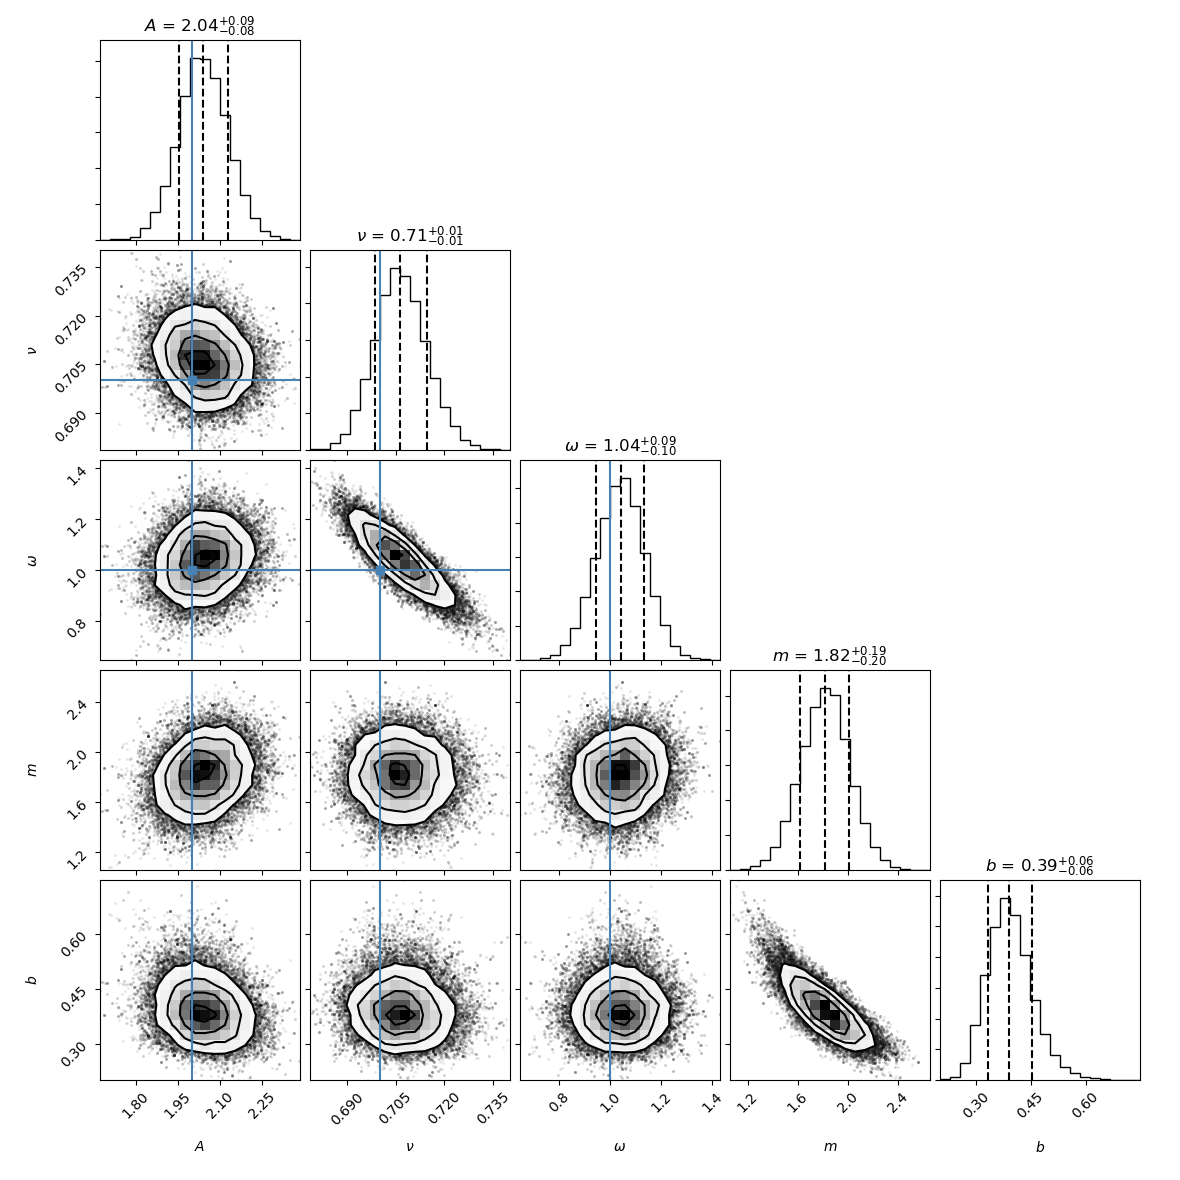
\includegraphics[width=\textwidth]{./Figures/Methods/Fitting_3-MCMC1_XY.png}
        \caption{Jitter correction applied}
    \end{subfigure}	
    \caption[Corner plots of MCMC]
    {Examples of two corner plots showing the successfully recovered planetary orbital parameters (to within 5\% of the true values for $A$ and $\nu$) with MCMC sampling. The blue solid lines indicate the true values of the input orbital parameters. The three dashed lines of each histogram are the corresponding median and $1\sigma$ boundaries. $A, \nu, \omega, \alpha$ and $\beta$ are the orbital amplitude, orbital frequency ratio, initial phase, the scaling factor for the jitter term and a radial velocity offset respectively.}
\label{fig:Corner}
\end{figure}    
%-------------

We did some test end-to-end simulations to investigate if the choice of the dividing frequency $\xi_{HL}$, or if having an overlapping frequency range such that $RV_\text{FT,L}$ is contributed by [0, $\xi_{HL1}$] and $RV_\text{FT,H}$ by [$\xi_{HL2}$, $\xi_H$] in which $\xi_{HL1} > \xi_{HL2}$, would make a difference in the overall performance of planet recoveries. Instead of equally dividing the power spectrum into the higher and lower frequencies as in the previous demonstrations, $\xi_{HL}$ chosen roughly one third of the cut-off frequency (resulting in about 85\% of power goes to $RV_\text{FT,L}$ and the other 15\% goes to $RV_\text{FT,H}$) tends to improve the successful recovery rate better than the other cases that we have tested and thus is used in the end-to-end simulations presented in this subsection. However, we have not drawn solid conclusions on a sweet spot for $\xi_{HL}$. 

%----------------------------------------------------------------------------------------
\subsection{Stellar jitter amplitude $\approx$ planetary amplitude}

The injected planet had the same parameter settings as in \S\ref{sec:check} (i.e. a circular orbit with amplitude $A = 2$~m/s, orbital frequency ratio $\nu = \nu_\text{orb}/\nu_\text{rot}= 0.7$ and initial phase $\omega = 1$~rad). For demonstration, we present two snapshots of each of the 500 trials of simulations with S/N = 10,000 and S/N = 2,000 (Fig.~\ref{fig:Planet_recovery_p2}). These are two examples where the planetary orbital parameters are correctly recovered (to within 10\% of the true values in each case). For S/N = 10,000, the discrepancy between the simulated radial velocities and the planet model is accounted for by the jitter model, and thus applying the jitter correction significantly reduces the rms of the residual. For S/N = 2,000, the fits are only slightly improved by introducing a jitter correction. The jitter model is not as accurate in the presence of moderate noise. 

%-------------
\begin{figure}[tbp]	
\centering
    \begin{subfigure}[b]{1.0\textwidth}
    		\begin{subfigure}[b]{0.49\textwidth}
        		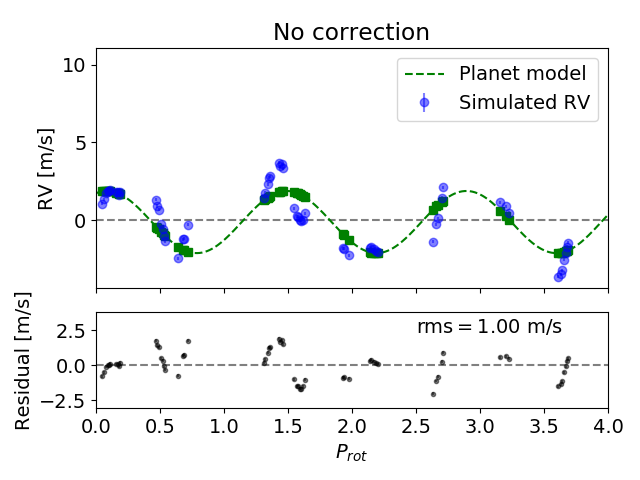
\includegraphics[width=\textwidth]{./Figures/Methods/Fitting_5-Fit2_SN10000.png}
		\end{subfigure}
		\begin{subfigure}[b]{0.49\textwidth}        		
        		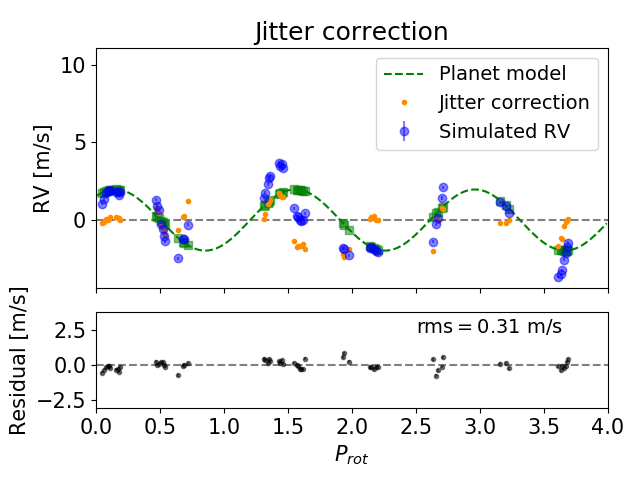
\includegraphics[width=\textwidth]{./Figures/Methods/Fitting_5-Fit1_XY_SN10000.png}
        	\end{subfigure}
        	\caption{S/N = 10,000}
    \end{subfigure}	       
    \begin{subfigure}[b]{1.0\textwidth}
    		\begin{subfigure}[b]{0.49\textwidth}
        		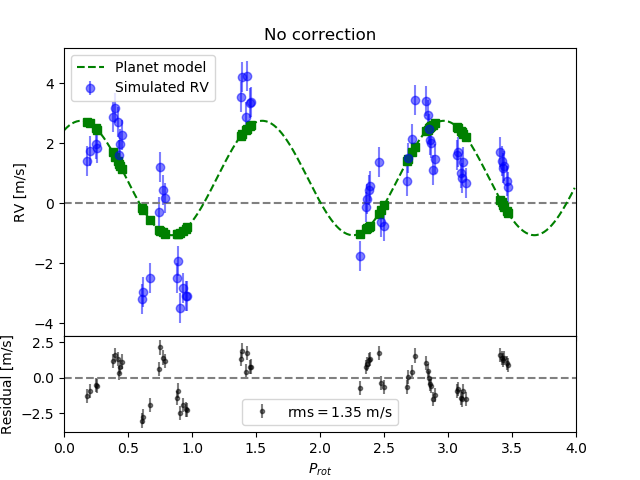
\includegraphics[width=\textwidth]{./Figures/Methods/Fitting_5-Fit2.png}
		\end{subfigure}
		\begin{subfigure}[b]{0.49\textwidth}        		
        		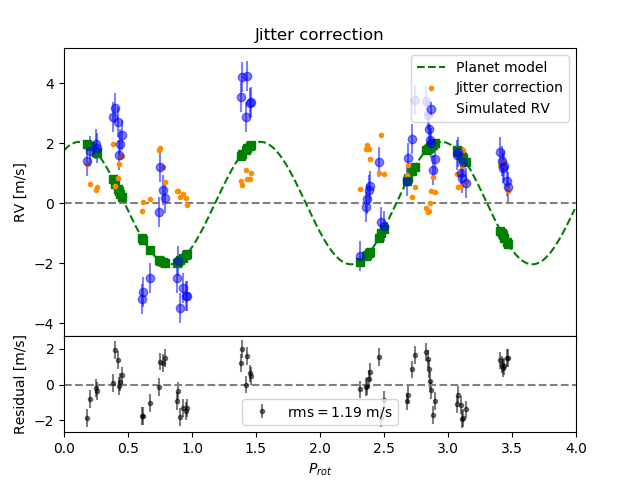
\includegraphics[width=\textwidth]{./Figures/Methods/Fitting_5-Fit1_XY.png}
        	\end{subfigure}
        	\caption{S/N = 2,000}
    \end{subfigure}	       
    \caption[Planet recovery ($A = 2$~m/s)]
    {One of the 500 trials of radial velocity fitting for $A = 2$~m/s. Top: S/N = 10,000; bottom: S/N = 2,000.}
\label{fig:Planet_recovery_p2}
\end{figure}    
%-------------

We show in Fig.~\ref{fig:Histogram} the histograms of the recovered orbital parameters for all 500 runs. To quantitatively describe this performance, we calculate the percentage of parameters successfully recovered within 5\% and 10\% of the true values as summarized in Table~\ref{table:a=2}. For example, for S/N = 10,000, 46\% of the 500 trials have both the amplitude ($A$) and orbital frequency ($\nu_\text{orb}/\nu_\text{rot}$) successfully recovered to within 5\% of the true parameters with jitter correction applied, while only 8\% achieve such a precision without jitter correction. 


%-------------
\begin{figure}[tbp]	
    \begin{subfigure}[b]{1.0\textwidth}
    		\begin{subfigure}[b]{0.49\textwidth}
        		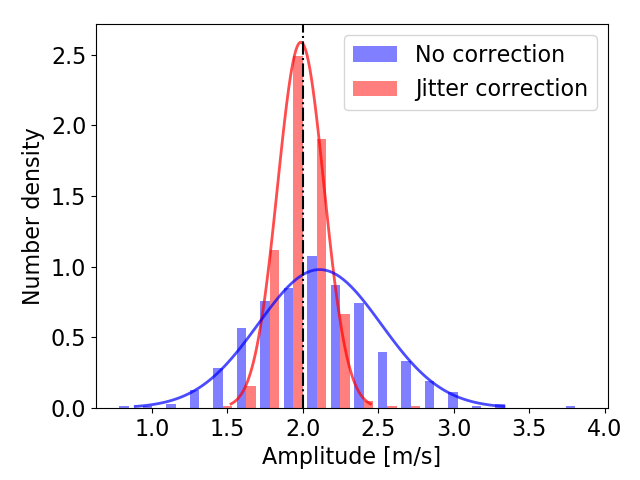
\includegraphics[width=\textwidth]{./Figures/Methods/Histogram_new1_p2_sn10000.png}
        \end{subfigure}
        \begin{subfigure}[b]{0.49\textwidth}
        		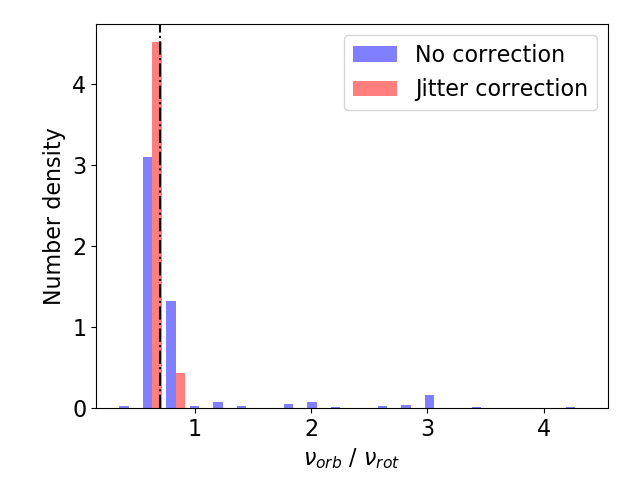
\includegraphics[width=\textwidth]{./Figures/Methods/Histogram_new2_p2_sn10000.png}
        \end{subfigure}
        \caption{S/N = 10,000}
    \end{subfigure}
    \begin{subfigure}[b]{1.0\textwidth}
    		\begin{subfigure}[b]{0.49\textwidth}
        		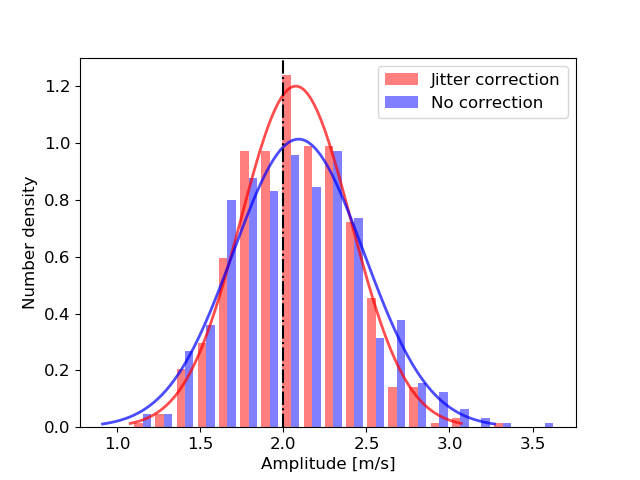
\includegraphics[width=\textwidth]{./Figures/Methods/Histogram_new1_p2_sn2000.png}
		\end{subfigure}
		\begin{subfigure}[b]{0.49\textwidth}        		
        		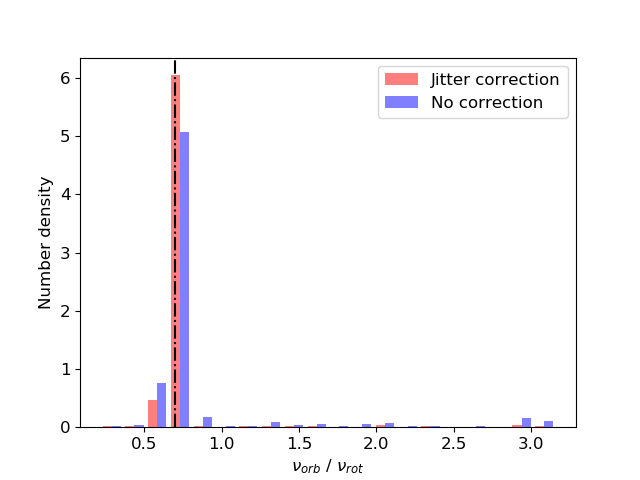
\includegraphics[width=\textwidth]{./Figures/Methods/Histogram_new2_p2_sn2000.png}
        	\end{subfigure}
        	\caption{S/N = 2,000}
    \end{subfigure}	       
    \caption[Histograms of recovered orbital parameters ($A = 2$~m/s)]
    {Histograms of recovered orbital parameters with a Gaussian profile fitted on top (where applicable).}
\label{fig:Histogram}
\end{figure}    
%-------------

%%-------------
\begin{table}[h!]
\centering
\begin{tabular}{|c|c|c|c|c|c|c|c|c|ll}
\cline{1-9}
\multirow{3}{*}{Percentage} & \multicolumn{4}{c|}{S/N = 10,000}                        & \multicolumn{4}{c|}{S/N = 2,000}                         &  &  \\ \cline{2-9}
                            & \multicolumn{2}{c|}{5\% limit} & \multicolumn{2}{c|}{10\% limit} & \multicolumn{2}{c|}{5\% limit} & \multicolumn{2}{c|}{10\% limit} &  &  \\ \cline{2-9}
                            				& $\dagger$     & $\ddagger$   & $\dagger$           & $\ddagger$           & $\dagger$           & $\ddagger$          & $\dagger$            & $\ddagger$          &  &  \\ \cline{1-9}
$A$                         					& 18\%            & 50\%           & 37\%            & 79\%            & 20\%            & 23\%           & 37\%             & 42\%           &  &  \\ \cline{1-9}
$\nu_\text{orb}/\nu_\text{rot}$              	& 53\%            & 93\%           & 78\%            & 100\%            & 49\%            & 66\%           & 77\%             & 91\%           &  &  \\ \cline{1-9}
both $A$ and $\nu_\text{orb}/\nu_\text{rot}$    & 8\%             & 46\%           & 27\%            & 79\%            & 10\%            & 16\%           & 28\%             & 38\%           &  &  \\ \cline{1-9}
\end{tabular}
\caption{Proportion of recovered parameters within 5\% and 10\% limit of $A = 2$~m/s and $\nu_\text{orb}/\nu_\text{rot} =0.7$. $\dagger$: no correction; $\ddagger$: jitter correction applied.}
\label{table:a=2}
\end{table}
%%-------------
\FloatBarrier

%----------------------------------------------------------------------------------------
\subsection{Planetary signal dominates}

In this case, we set the orbital amplitude to be $A = 20$~m/s (Fig.~\ref{fig:Planet_recovery_p20}). Both fits with, and without, the aid of jitter correction manage to recover almost all the planetary orbital parameters to within 5\% accuracy (Fig.~\ref{fig:Histogram20} and Table.~\ref{table:a=20}). Implementing jitter correction with $\mathit{\Phi}$ESTA further improves the performance, especially in high S/N (=~10,000) showing 61\% of the orbital parameters are recovered up to 1\% accuracy, compared with a mere 30\% without jitter correction. 

%-------------
\begin{figure}[tbp]	
\centering
    \begin{subfigure}[b]{1.0\textwidth}
    		\begin{subfigure}[b]{0.49\textwidth}
        		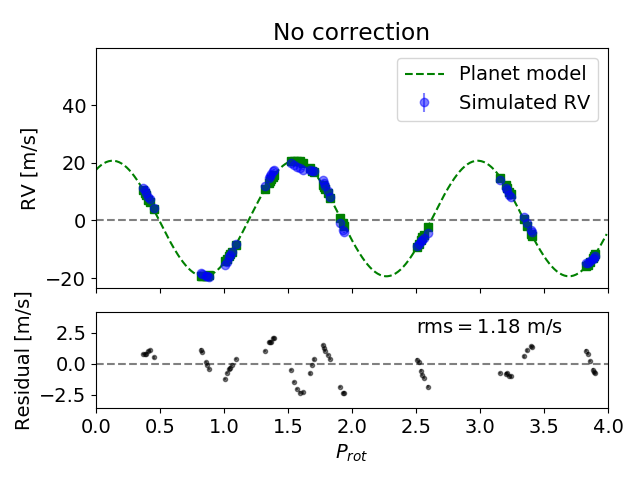
\includegraphics[width=\textwidth]{./Figures/Methods/Fitting_5-Fit2_a20_SN10000.png}
		\end{subfigure}
		\begin{subfigure}[b]{0.49\textwidth}        		
        		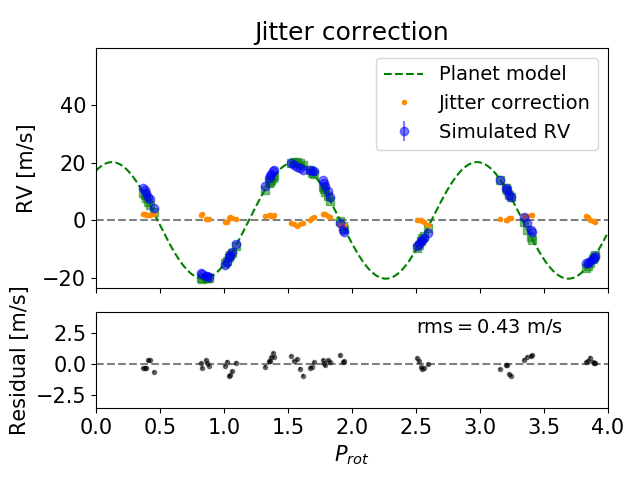
\includegraphics[width=\textwidth]{./Figures/Methods/Fitting_5-FitZX_a20_SN10000.png}
        	\end{subfigure}
        	\caption{S/N = 10,000}
    \end{subfigure}	       
    \begin{subfigure}[b]{1.0\textwidth}
    		\begin{subfigure}[b]{0.49\textwidth}
        		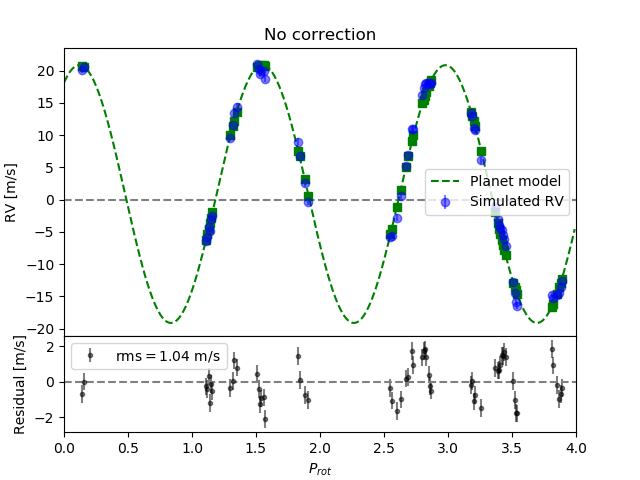
\includegraphics[width=\textwidth]{./Figures/Methods/Fitting_5-Fit2_a20.png}
		\end{subfigure}
		\begin{subfigure}[b]{0.49\textwidth}        		
        		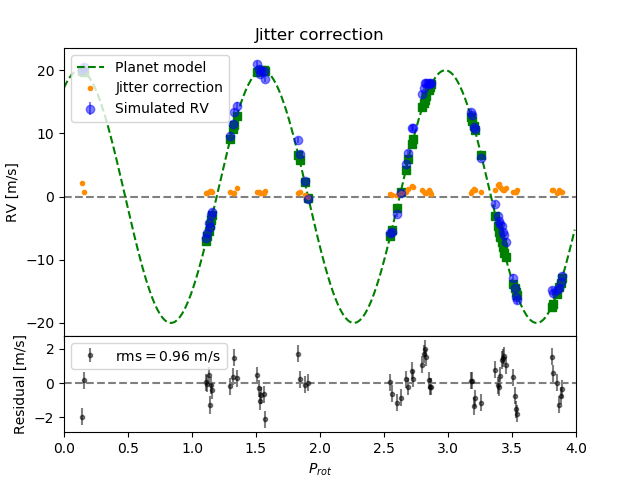
\includegraphics[width=\textwidth]{./Figures/Methods/Fitting_5-Fit1_XYZ_a20.png}
        	\end{subfigure}
        	\caption{S/N = 2,000}
    \end{subfigure}	       
    \caption[Planet recovery ($A = 20$~m/s)]
    {Same with Fig.~\ref{fig:Planet_recovery_p2} but for $A = 20$~m/s.}
\label{fig:Planet_recovery_p20}
\end{figure}    
%-------------


%-------------
\begin{figure}[tbp]	
    \begin{subfigure}[b]{1.0\textwidth}
    		\begin{subfigure}[b]{0.49\textwidth}
        		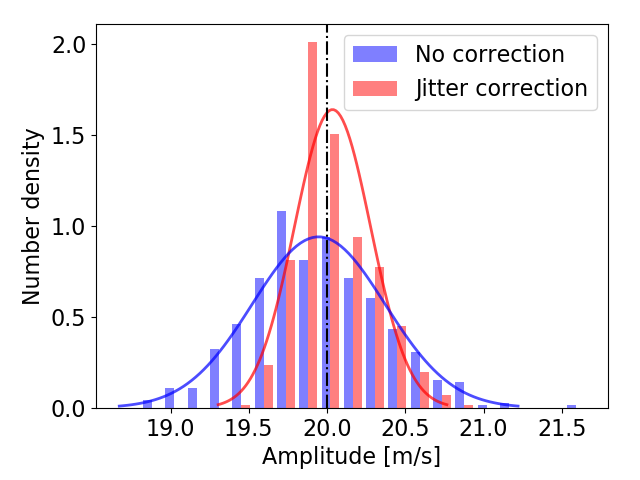
\includegraphics[width=\textwidth]{./Figures/Methods/Histogram_new1_p20_sn10000.png}
        \end{subfigure}
        \begin{subfigure}[b]{0.49\textwidth}
        		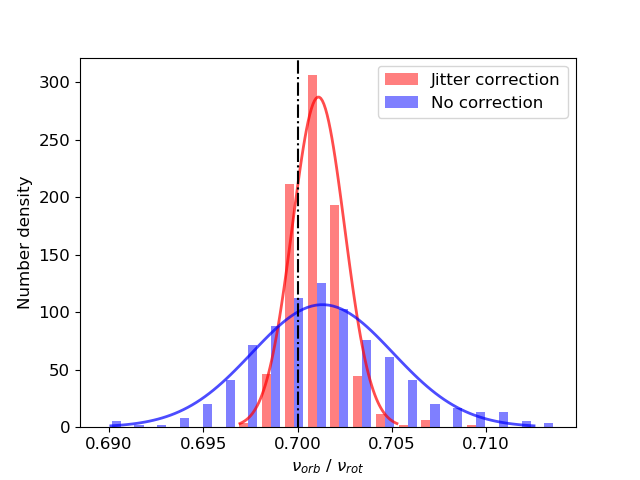
\includegraphics[width=\textwidth]{./Figures/Methods/Histogram_new2_p20_sn10000.png}
        \end{subfigure}
        \caption{S/N = 10,000}
    \end{subfigure}
    \begin{subfigure}[b]{1.0\textwidth}
    		\begin{subfigure}[b]{0.49\textwidth}
        		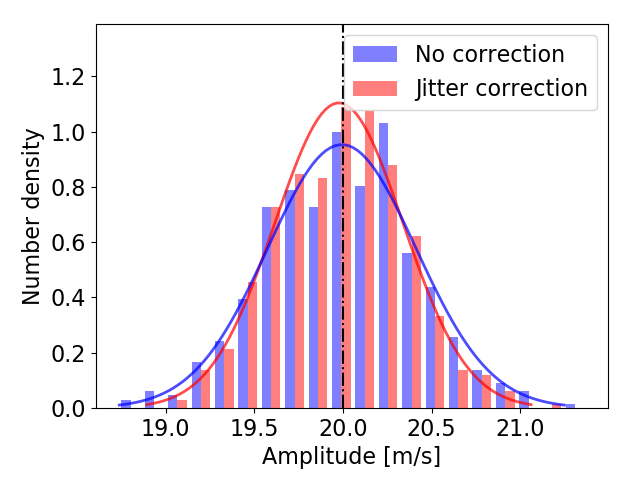
\includegraphics[width=\textwidth]{./Figures/Methods/Histogram_new1_p20_sn2000.png}
		\end{subfigure}
		\begin{subfigure}[b]{0.49\textwidth}        		
        		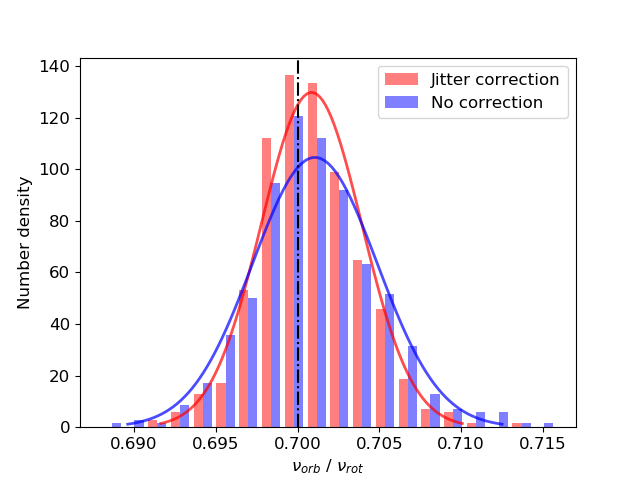
\includegraphics[width=\textwidth]{./Figures/Methods/Histogram_new2_p20_sn2000.png}
        	\end{subfigure}
        	\caption{S/N = 2,000}
    \end{subfigure}	       
    \caption[Histogram of recovered orbital parameters ($A = 20$~m/s)]
    {Same with Fig.~\ref{fig:Histogram} but for $A = 20$~m/s.}
\label{fig:Histogram20}
\end{figure}    
%-------------

%-------------
\begin{table}[h!]
\centering
\begin{tabular}{|c|c|c|c|c|c|c|c|c|ll}
\cline{1-9}
\multirow{3}{*}{Percentage} & \multicolumn{4}{c|}{S/N = 10,000}                        & \multicolumn{4}{c|}{S/N = 2,000}                         &  &  \\ \cline{2-9}
                            & \multicolumn{2}{c|}{1\% limit} & \multicolumn{2}{c|}{5\% limit} & \multicolumn{2}{c|}{1\% limit} & \multicolumn{2}{c|}{5\% limit} &  &  \\ \cline{2-9}
                            				& $\dagger$     & $\ddagger$   & $\dagger$           & $\ddagger$           & $\dagger$           & $\ddagger$          & $\dagger$            & $\ddagger$          &  &  \\ \cline{1-9}
$A$                         					& 33\%            & 61\%           & 99\%            & 100\%            & 34\%            & 40\%           & 98\%             & 100\%           &  &  \\ \cline{1-9}
$\nu_\text{orb}/\nu_\text{rot}$              	& 92\%            & 100\%           & 100\%            & 100\%            & 93\%            & 96\%           & 100\%             & 100\%           &  &  \\ \cline{1-9}
both $A$ and $\nu_\text{orb}/\nu_\text{rot}$    & 30\%             & 61\%           & 99\%            & 100\%            & 31\%            & 38\%           & 98\%             & 100\%           &  &  \\ \cline{1-9}
\end{tabular}
\caption{Proportion of recovered parameters within 1\% and 5\% limit of $A = 20$~m/s and $\nu_\text{orb}/\nu_\text{rot} =0.7$. $\dagger$: no correction; $\ddagger$: jitter correction applied.}
\label{table:a=20}
\end{table}
%-------------

\FloatBarrier

%----------------------------------------------------------------------------------------
\subsection{Stellar jitter only}

We set $A=0$~m/s so that the measured the radial velocity only comes from stellar variability. We fit the data by the sum of a Keplerian orbit and a jitter correction model to see if a null planet solution can be returned, i.e. a recovered planetary amplitude lying at or being smaller than the noise level of the data.

We remind ourselves that the spot configuration in Table~\ref{table:spot_configurations} is used. Three starspots appear and disappear in turns (Fig.~\ref{fig:rv_recovery_deformed}), mimicking the radial velocities of orbiting exoplanets. This is seen in the histogram of ``recovered" orbital parameters (Fig.~\ref{fig:Histogram_null}), where three peaks occur at $\nu_\text{orb}/\nu_\text{rot} =$ 1, 2 and 3, with $\nu_\text{orb}/\nu_\text{rot} = 3$ being the most prominent. Applying the jitter correction, the overall amplitudes (calculated from the centre of a Gaussian fit on the distribution of amplitudes) of the ``recovered" planet is effectively reduced from 1.32~m/s to 0.54~m/s for S/N = 10,000, but only marginally decreased from 1.33~m/s to 1.14~m/s for S/N = 2,000, and neither of them reaches below the rms of photon noise level: $\sim 0.1$~m/s for S/N = 10,000 and $\sim 0.5$~m/s for S/N = 2,000. As a result, we still cannot negate such a signal with a reduced amplitude with this approach alone. 

%-------------
\begin{figure}[tbp]	
    \begin{subfigure}[b]{1.0\textwidth}
    		\begin{subfigure}[b]{0.49\textwidth}
        		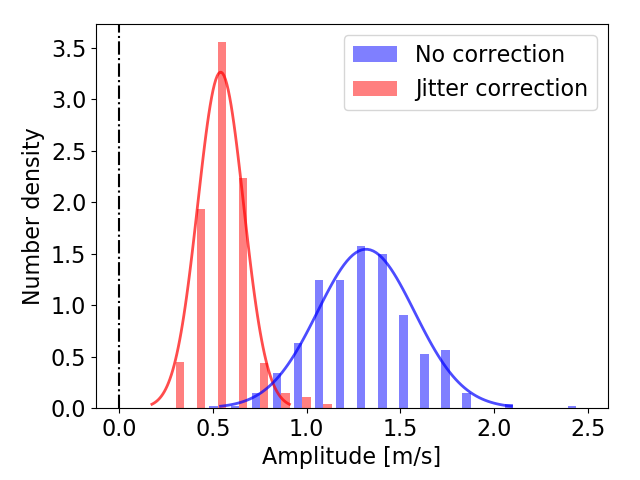
\includegraphics[width=\textwidth]{./Figures/Methods/Histogram_new1_null_10000.png}
        \end{subfigure}
        \begin{subfigure}[b]{0.49\textwidth}
        		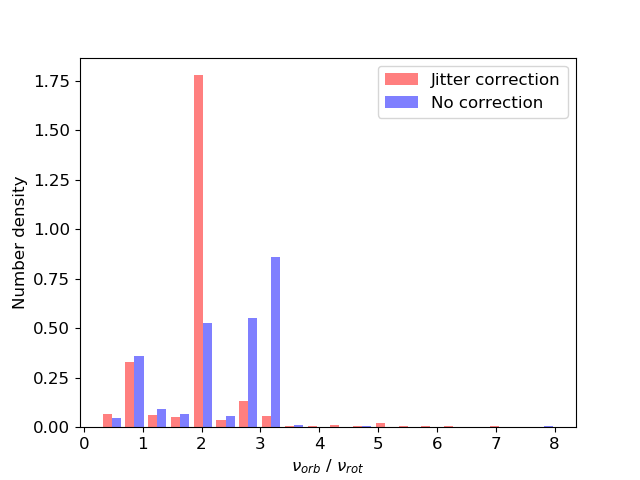
\includegraphics[width=\textwidth]{./Figures/Methods/Histogram_new2_null_10000.png}
        \end{subfigure}
        \caption{S/N = 10,000}
    \end{subfigure}
    \begin{subfigure}[b]{1.0\textwidth}
    		\begin{subfigure}[b]{0.49\textwidth}
        		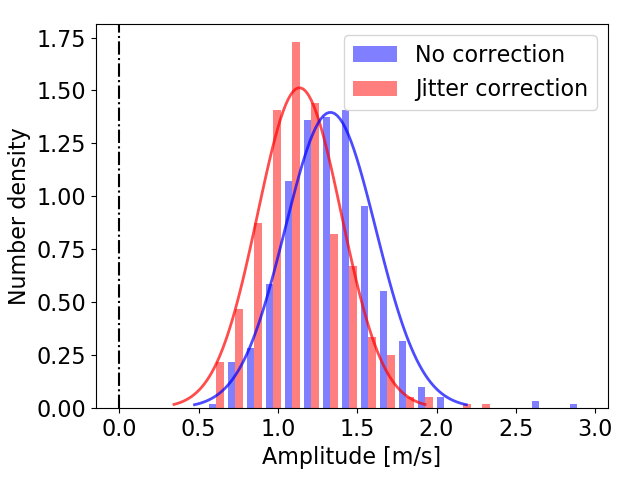
\includegraphics[width=\textwidth]{./Figures/Methods/Histogram_new1_null_2000.png}
		\end{subfigure}
		\begin{subfigure}[b]{0.49\textwidth}        		
        		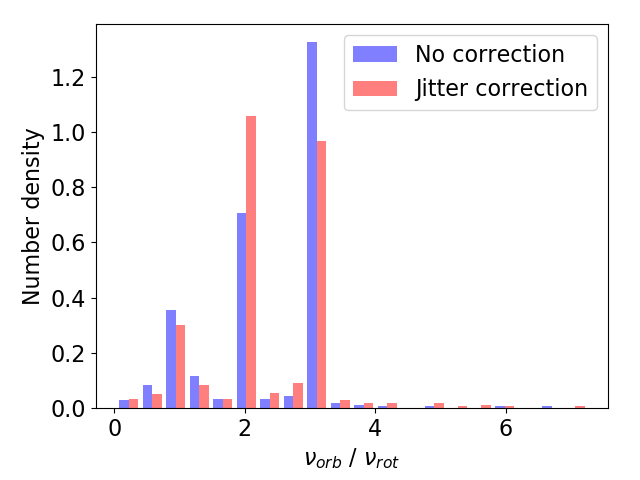
\includegraphics[width=\textwidth]{./Figures/Methods/Histogram_new2_null_2000.png}
        	\end{subfigure}
        	\caption{S/N = 2,000}
    \end{subfigure}	       
    \caption[Histogram of recovered orbital parameters of null planets]
    {Histogram of ``recovered" orbital parameters in null planet end-to-end simulations.}
\label{fig:Histogram_null}
\end{figure}    
%-------------

\FloatBarrier

%----------------------------------------------------------------------------------------
\subsection{Classification}
\label{sec:Classification}

We can demonstrate the use of the relations among $RV_\text{Gaussian}$, $RV_\text{FT,H/L}$ and $\Delta RV_\text{H/L}$ to classify the relative magnitudes of jitter and planetary signals. 

In Fig.~\ref{fig:correlations}, 4 combinations of relative sizes between jitter and planetary signal are displayed. In (a), (b) and (c) where stellar jitter is present, a well defined linear correlation can be seen between $\Delta RV_\text{H}$ and $\Delta RV_\text{L}$. Both $\Delta RV_\text{H}$ and $\Delta RV_\text{L}$ are used as jitter metrics. They are linearly correlated with jitter and thus proportional to each other as well. 

%-------------
\begin{figure}[htbp]	
    \begin{subfigure}[b]{1.0\textwidth}
        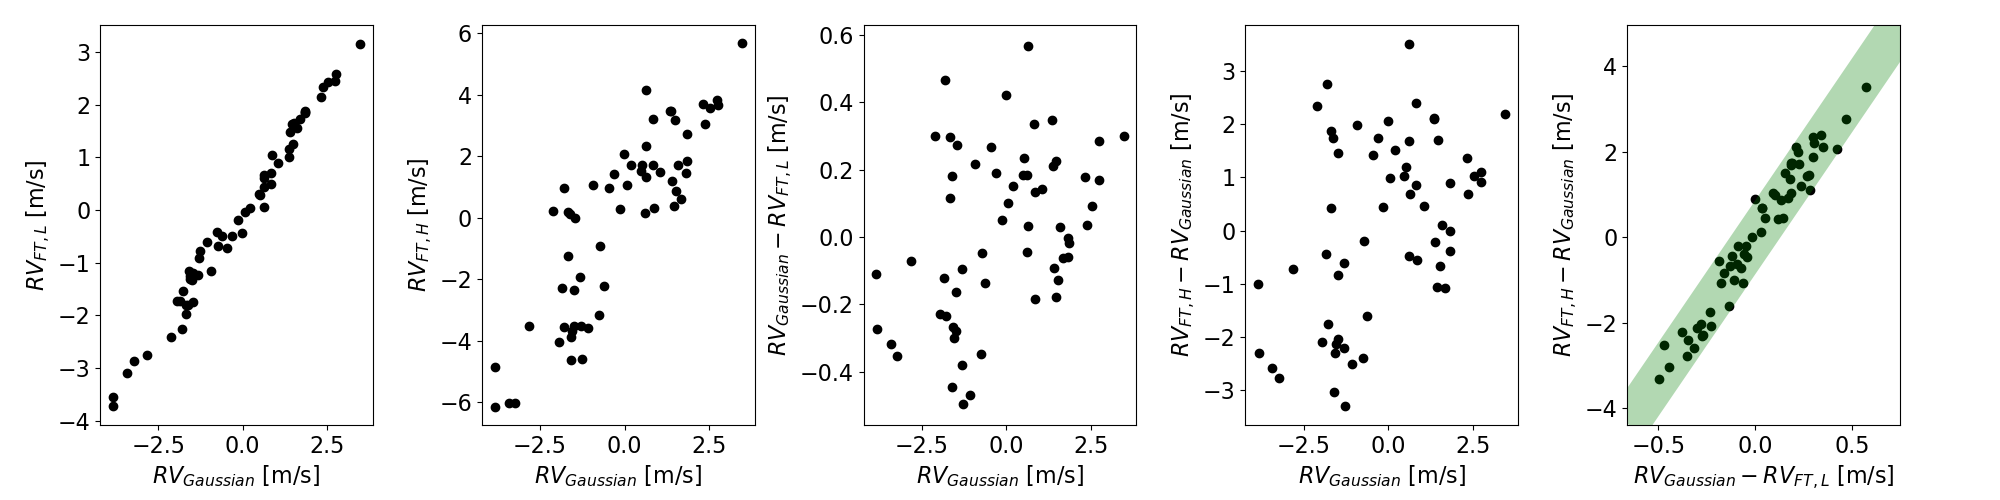
\includegraphics[width=\textwidth]{./Figures/Methods/Correlation_2pj.png}
        \caption{Stellar jitter amplitude $\approx$ planetary amplitude.}
    \end{subfigure}
	~
    \begin{subfigure}[b]{1.0\textwidth}
        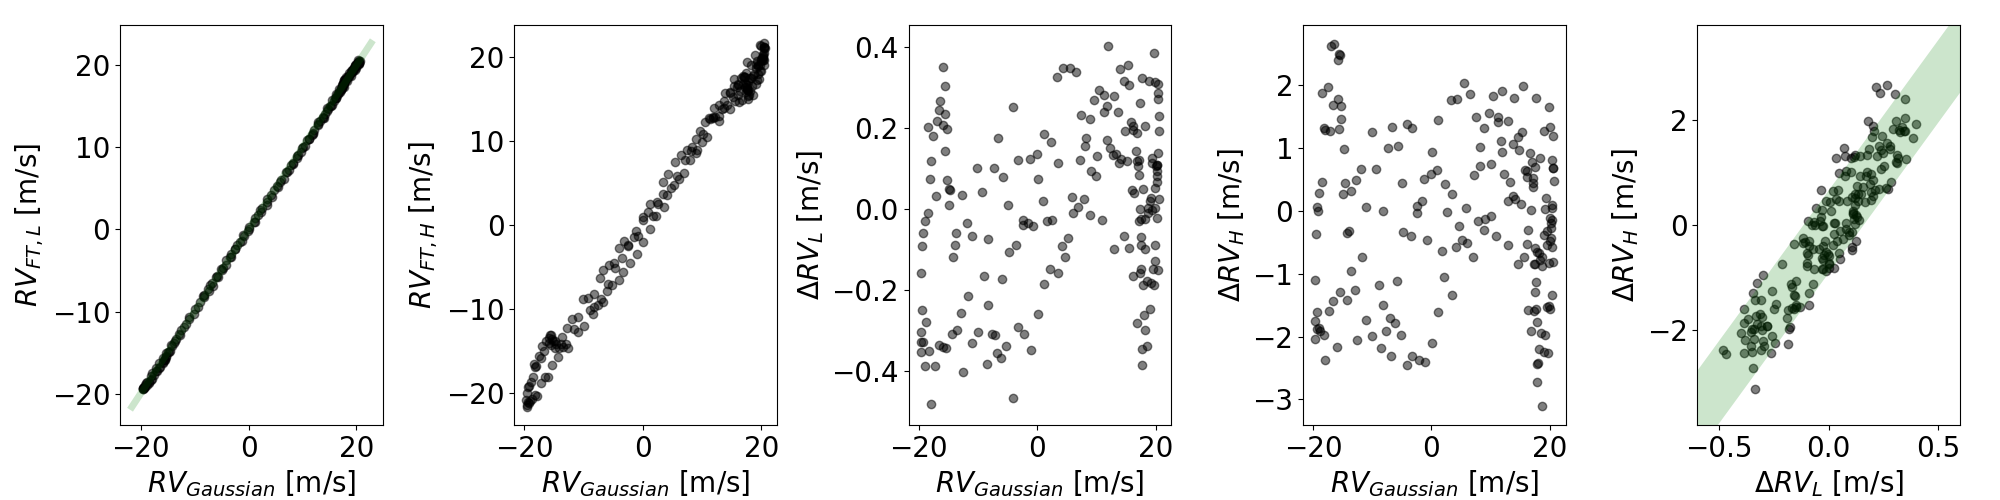
\includegraphics[width=\textwidth]{./Figures/Methods/Correlation_20pj.png}
        \caption{Planetary signal dominating.}
    \end{subfigure}	
	~
    \begin{subfigure}[b]{1.0\textwidth}
        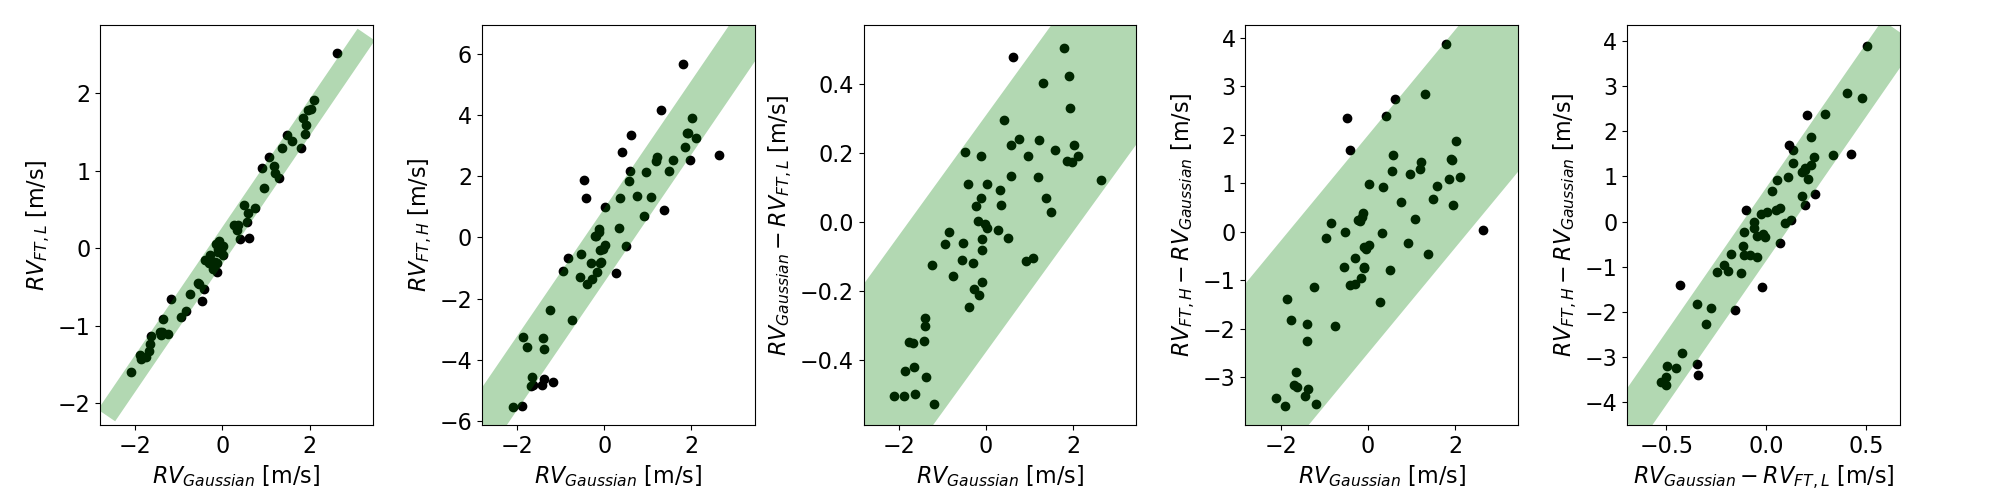
\includegraphics[width=\textwidth]{./Figures/Methods/Correlation_null.png}
        \caption{Jitter only; no planet.}
    \end{subfigure}	    
	~
    \begin{subfigure}[b]{1.0\textwidth}
        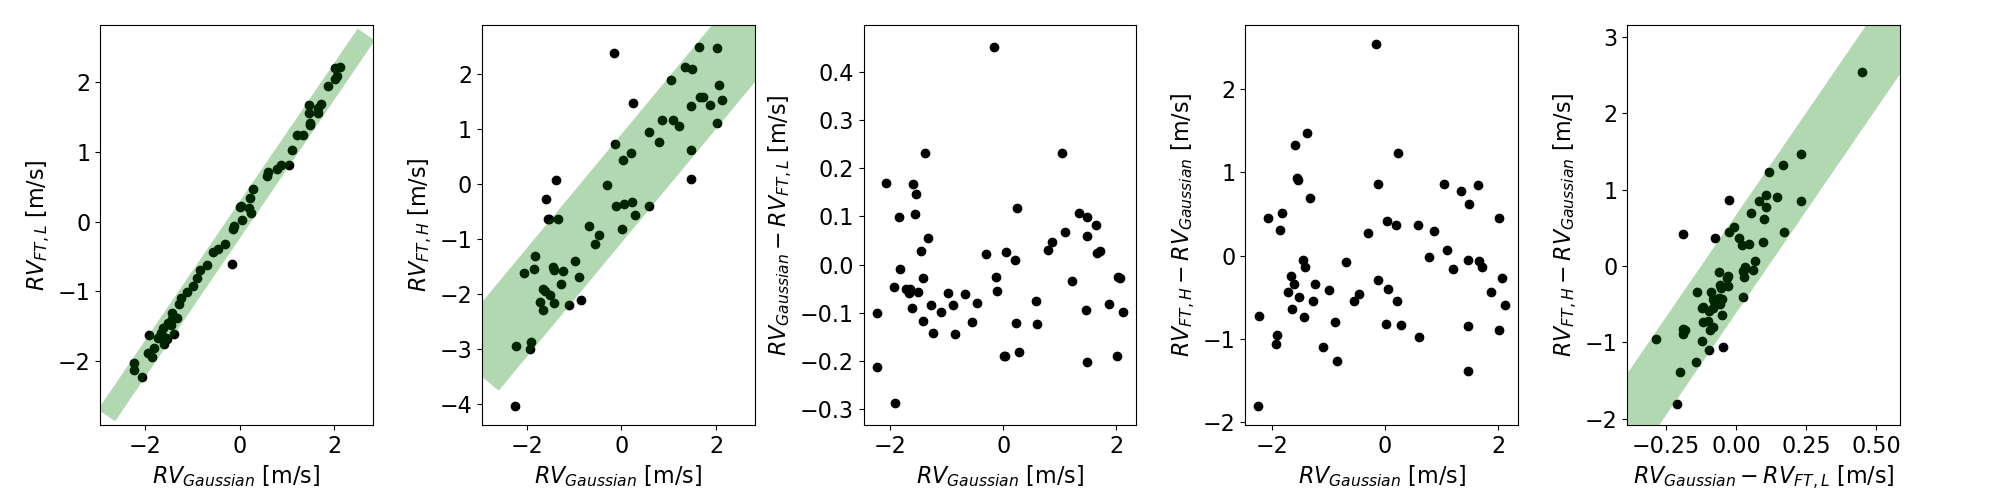
\includegraphics[width=\textwidth]{./Figures/Methods/Correlation_0jitter.png}
        \caption{Planet only; ``no" jitter.}
    \end{subfigure}	    
    \caption[Classification of jitter dominated or planetary signal dominated]        
    {Classifications for the relative magnitudes of jitter and planetary radial velocity signals. The green trends show the linear correlations that are expected from each configuration.}
\label{fig:correlations}
\end{figure}    
%-------------

The respective features that distinguish each from the others in the four panels are follows.
\begin{enumerate}[label=(\alph*)]
	\item Stellar jitter amplitude $\approx$ planetary amplitude:
	\begin{itemize}
		\item a decent linear relation between $RV_\text{FT,L}$ and $RV_\text{Gaussian}$, as they only differ by $\Delta RV_\text{L}$, some 20\% of the jitter, a small amount compared to $RV_\text{FT,L}$ and $RV_\text{Gaussian}$;
		\item a weakly related trend between $RV_\text{FT,H}$ and $RV_\text{Gaussian}$, as they differ by $\Delta RV_\text{H}$, which is at the magnitude of jitter;
		\item weakly related trends in $\Delta RV_\text{L}$ or $\Delta RV_\text{H}$ verses $RV_\text{Gaussian}$, which can be seen as a well correlated $\Delta RV_\text{H}$ or $\Delta RV_\text{L}$ versus the jitter with the planetary radial velocity on top of jitter adding x-dispersion;
	\end{itemize}
	
	\item Planetary signal dominating:
	\begin{itemize}
		\item a tight linear correlation between $RV_\text{FT,L}$ and $RV_\text{Gaussian}$ (same reasoning as above but the difference between the two axes -- some 20\% of the jitter -- is even relatively smaller compared to the size of $RV_\text{FT,L}$ and $RV_\text{Gaussian}$);
		\item a somewhat tight linear correlation between $\Delta RV_\text{H}$ and $RV_\text{Gaussian}$ (same reasoning as above but the difference between the two axes is at the magnitude of jitter);
		\item no correlation between $\Delta RV_\text{H}$ or $\Delta RV_\text{L}$ verses $RV_\text{Gaussian}$, as the x-axes are dominated by the planetary signal, while the y-axes are solely the jitter metrics;
	\end{itemize}
	
	\item Only jitter and no planet:
	\begin{itemize}
		\item all panels show linear correlations, as $RV_\text{Gaussian}$ directly measures jitter when no planet is present, and it is linearly correlated with $RV_\text{FT,L}$, $RV_\text{FT,H}$, $\Delta RV_\text{L}$ and $\Delta RV_\text{H}$. 
	\end{itemize}

	\item Only planet and ``no" jitter:
	\begin{itemize}
		\item 1:1 linear correlations between $RV_\text{FT,L}$ or $RV_\text{FT,H}$ and $RV_\text{Gaussian}$, as they all measure the planetary radial velocities when jitter is absent;
		\item no correlation between $\Delta RV_\text{H}$ or $\Delta RV_\text{L}$ verses $RV_\text{Gaussian}$, as the jitter metrics $\Delta RV_\text{L}$ and $\Delta RV_\text{H}$ fluctuate as a result of photon noise; in other words, there is no intrinsic difference among the line profile shapes, but photon noise is interpreted as a ``deformation" in the jitter metrics;
		\item no expected correlation between $\Delta RV_\text{H}$ and $\Delta RV_\text{L}$, as both are simply measurements of line deformation due to photon noise. In lower S/N circumstances or inconsistent cross-correlations among line profiles, a linear correlation may be seen, as the ``deformation" becomes more detectable.  
	\end{itemize}	

\end{enumerate}

We note that these features are based on a high S/N (=~10,000) simulation. In lower S/N circumstances, such correlations will be less obvious as the data becomes more scattered. However, a simulation at a corresponding S/N can be reproduced and used as a reference. 


%----------------------------------------------------------------------------------------
\subsection{Periodogram analysis with $\mathit{\Phi}$ESTA}

We can use the Lomb-Scargle periodogram (tool available in \verb|astropy|) in combination with $\mathit{\Phi}$ESTA to address the problem of stellar jitter mimicking planetary signals. The idea is to compare the periodogram of the measured radial velocities (i.e. $RV_\text{Gaussian}$) and that of the jitter metrics (i.e. $\Delta RV_\text{H}$ and $\Delta RV_\text{L}$) that correlate with jitter. Peaks of the jitter metrics periodogram are likely to indicate periodicities associated with jitter. 

We generated 400 radial velocities samples in four stellar rotations (i.e. no sub-sampling) from the two sets of data: (1) stellar jitter amplitude $\approx$ planetary amplitude and (2) stellar jitter only, that had the same spot and orbital configuration as the previous end-to-end simulations. We chose a moderate S/N = 2,000 for cross-correlation profiles and no smoothing of radial velocity data was applied. 

Fig.~\ref{fig:Periodogram} shows an example of the application of periodogram analysis with the $\mathit{\Phi}$ESTA jitter metrics. In Fig.~\ref{fig:Periodogram1} the planetary orbital frequency $\nu_\text{orb}/\nu_\text{rot} = 0.7$ stands out clearly while the other prominent peaks coincide with those of the jitter metrics. This shows that the $\mathit{\Phi}$ESTA jitter metrics can disentangle jitter from planetary components in the radial velocities. In the case of a null planet (Fig.~\ref{fig:Periodogram2}), all the possible candidates where the $RV_\text{Gaussian}$ peaks occur are also indicated to be sources of periodicity due to the jitter. 

%-------------
\begin{figure}[tbp]	
    \begin{subfigure}[b]{0.49\textwidth}
        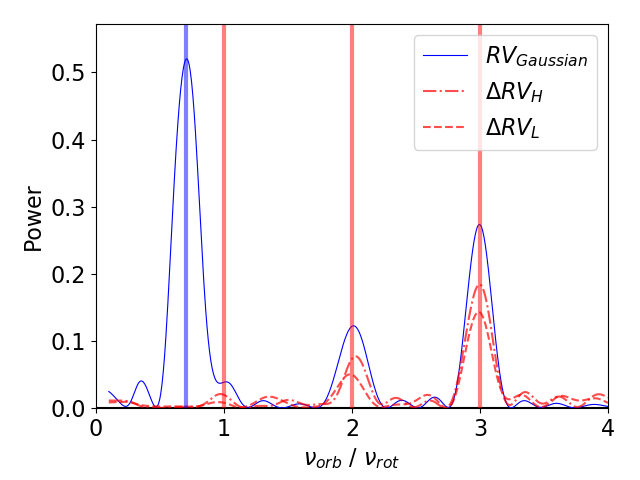
\includegraphics[width=\textwidth]{./Figures/Methods/0-Periodogram_1.png}
        \caption{Jitter amplitude $\approx$ planetary amplitude}
        \label{fig:Periodogram1}
    \end{subfigure}
	~
    \begin{subfigure}[b]{0.49\textwidth}
        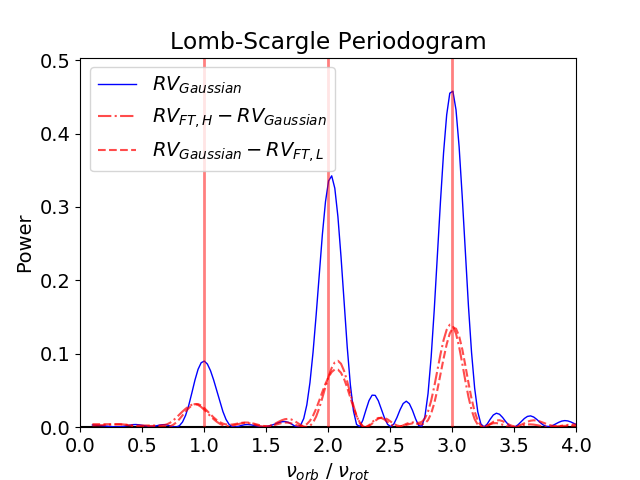
\includegraphics[width=\textwidth]{./Figures/Methods/0-Periodogram_2.png}
        \caption{Stellar jitter only}
        \label{fig:Periodogram2}
    \end{subfigure}	
    \caption[Periodogram combined with $\mathit{\Phi}$ESTA]
    {Periodogram of $RV_\text{Gaussian}$ and the jitter metrics $\Delta RV_\text{H}$ and $\Delta RV_\text{L}$. The single prominent peak in (a) indicates the orbital frequency (or period) of the injected planet. The true orbital frequency is labelled as the blue vertical line $\nu_\text{orb}/\nu_\text{rot} = 0.7$; the suspicious frequencies are labelled in red vertical lines at $\nu_\text{orb}/\nu_\text{rot} =$ 1, 2 and 3. The normalization mode of periodogram is standard as default.}
\label{fig:Periodogram}
\end{figure}    
%-------------



\pagebreak
%----------------------------------------------------------------------------------------	
%----------------------------------------------------------------------------------------	
\section{Applying $\mathit{\Phi}$ESTA on real observations}
\label{\thesection}
\label{sec:observation}

\subsection{HD189733: the Rossiter–McLaughlin effect as jitter}
\label{sec:HD189733}

HD189733 is a well studied binary star system. The main star HD189733~A is known to host a gas giant exoplanet HD189733~b, first detected by transits and subsequently confirmed by Doppler spectroscopy \cite{Bouchy2005ELODIE}. The Rossiter–McLaughlin effect (Fig.~\ref{fig:rm-effect}), is an apparent change in radial velocity produced when the planet passes in front of its parent star, and has been studied in \cite{Cochran2006} and \cite{Triaud2009}. During the eclipse, the planet breaks the observed flux symmetry of the stellar photosphere and produce an asymmetric spectral line profile and apparent radial velocity shift.

%-------------
\begin{figure}[htbp]
\centering
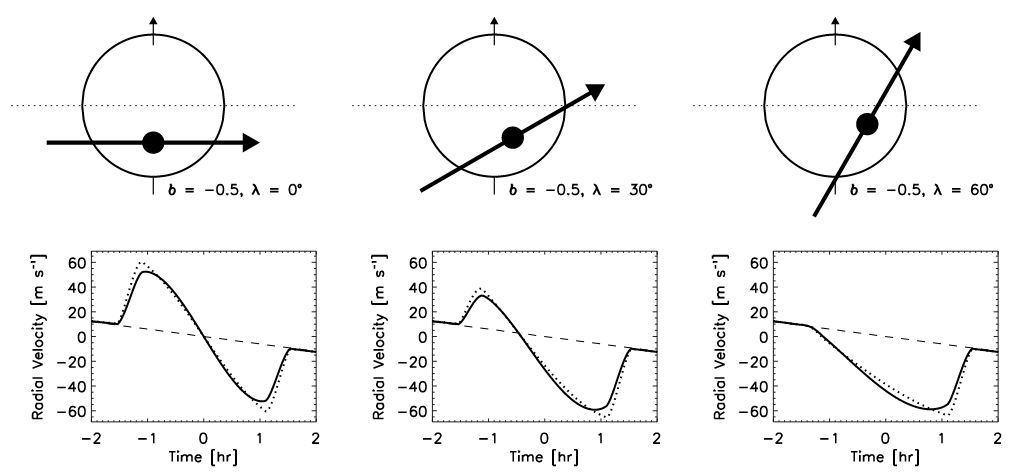
\includegraphics[width = 0.80 \linewidth]
{./Figures/Methods/rmeffect.png}
\caption[The Rossiter–McLaughlin effect]
{The Rossiter–McLaughlin effect (figure taken from \cite{Gaudi2007}) is an apparent radial velocity change of the parent star due to an eclipsing companion (either a star or a planet). This plot shows three different star-planet alignments and the corresponding different forms of Rossiter–McLaughlin curves for each. The solid line is the model including limb darkening, and the dotted line without limb darkening.}
\label{fig:rm-effect}
\end{figure} 
%-------------

We aim to test if jitter estimates generateed by $\mathit{\Phi}$ESTA can account for the apparent radial velocity shift of the Rossiter–McLaughlin effect. We choose this target as a case study for the following reasons: (1) HD189733~b is a confirmed transiting exoplanet, so that we know what to expect from the radial velocity shift during the eclipse. (2) The gas giant exoplanet causes a prominent apparent radial velocity shift as it transits (amplitude up to $\sim 40$~m/s), making it the dominant radial velocity shift (although the star itself exhibits signs of activity \cite{Boisse189733}, \cite{Cauley2017}). (3) The system HD189733 has a visual magnitude of $V\sim7.65$ \cite{SIMBAD189733} (or $G=7.41$ from the Gaia archive), dominated by the primary host star HD189733~A, and therefore a moderate S/N (2000-4000) in the HARPS cross-correlation profile, which is required for $\mathit{\Phi}$ESTA in recovering radial velocities.

There are a few HD189733~b transiting radial velocity segments in the HARPS archive. In particular, we present the one with Julian dates from 2454340.98 to 2454341.11 because it covers both the non-transiting and transiting part of the radial velocity curve and has relatively higher cadence of observing. The cross-correlation of the spectral lines of this segment were constructed by a G2 template by HARPS. We also tested our method in the segment with Julian dates from 2453986.00 to 2453986.17, the cross-correlation profiles of which were constructed by a K5 template, but with about half the observing cadence -- it also returns similar performance on fitting the Rossiter–McLaughlin effect by the $\mathit{\Phi}$ESTA jitter metrics.

Here we briefly recap the procedure for obtaining the ``jitter" model derived by $\mathit{\Phi}$ESTA. $RV_\text{HARPS}$ were obtained from the HARPS spectra headers (consistent with $RV_\text{Gaussian}$ by fitting a Gaussian function to the line profile and $RV_\text{FT}$ derived from the full Fourier phase spectrum); $RV_\text{FT,H}$ and $RV_\text{FT,L}$ were derived from the corresponding part of the Fourier phase spectrum of HARPS cross-correlation line profiles (Fig.~\ref{fig:HD189733} upper left). We could then obtain the raw jitter metrics $\Delta RV_\text{H} = RV_\text{FT,H} - RV_\text{HARPS}$ and $\Delta RV_\text{L} = RV_\text{HARPS} - RV_\text{FT,L}$ (Fig.~\ref{fig:HD189733} lower left). We show only the processes from $\Delta RV_\text{L}$ as the jitter model built from $\Delta RV_\text{H}$ can be obtained in the same procedure and presents similar results. The inclined trend of the radial velocity curve is attributed to the exoplanet (with an orbital period is estimated 2.219 days \cite{Bouchy2005ELODIE}) as well as the companion binary star HD189733~B (with an orbital period $\approx$ 3,200 years \cite{Bakos2006}) -- both orbiting time-scales are long enough compared to the $\sim$ 2 hour planetary transit. Therefore a local approximation can be applied by fitting a linear trend onto the non-transiting part of the radial velocities. This is then removed to leave the residual Rossiter–McLaughlin curve (Fig.~\ref{fig:HD189733} upper right) and treated as ``jitter" and modelled by the raw jitter metric multiplied by a scaling factor. 

%-------------
\begin{figure}[tbp]
\centering
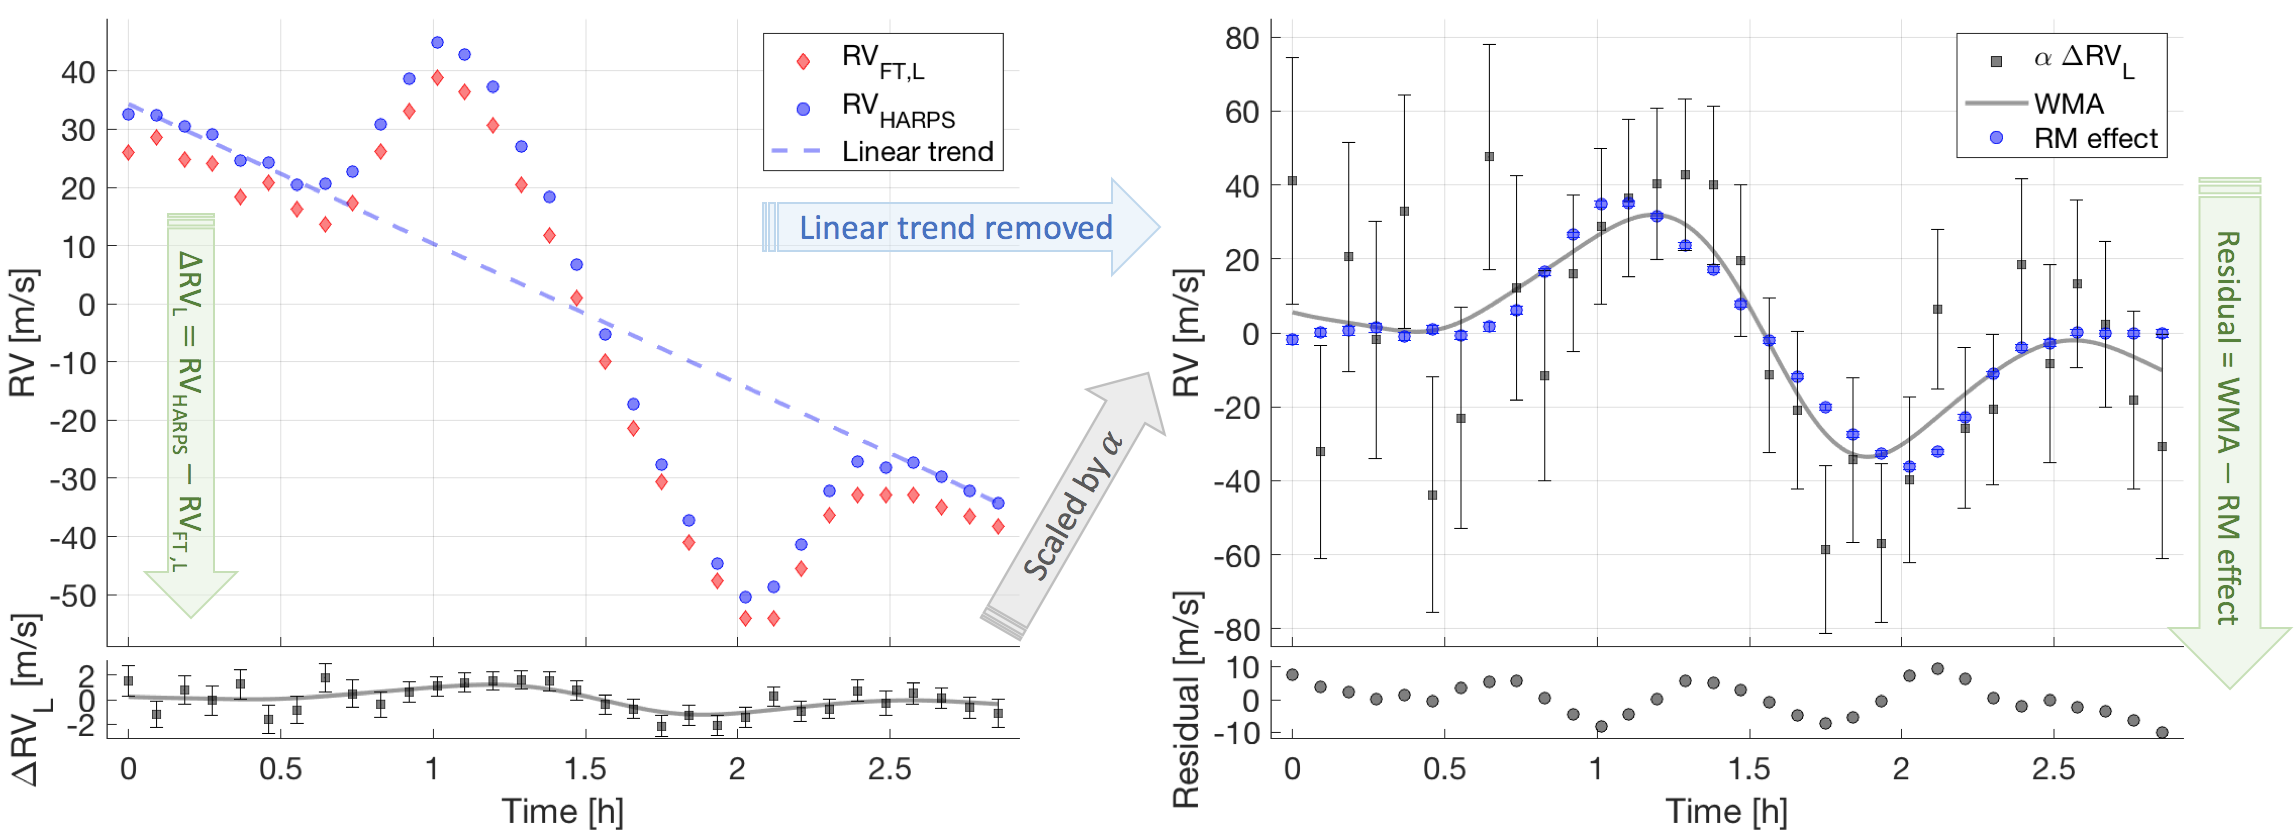
\includegraphics[width = 1.0 \linewidth]
{./Figures/Methods/HD189733.png}
\caption[HD189733: modelling Rossiter–McLaughlin effect as jitter]
		{Flowchart of modelling the Rossiter–McLaughlin effect as jitter using $\mathit{\Phi}$ESTA on HD189733. Note that $RV_\text{FT,L}$ is offset by 5~m/s to avoid visual overlap with $RV_\text{HARPS}$ in the upper left panel. The errorbars related to the radial velocities from $\mathit{\Phi}$ESTA (e.g. $\Delta RV_\text{L}$) are only correct relative to each other (as derived from the photon noise) but not evaluated in the absolute scale.}
\label{fig:HD189733}
\end{figure} 
%-------------

The scaled model is then smoothed using a weighted moving average (WMA) with $\tau~\sim0.2$ hour (twice of the spacing of two consecutive observations). Although required to mitigate against the phase noise sensitivity of $\mathit{\Phi}$ESTA, this does smear the drastic velocity change seen when the planet enters and departs the stellar disk. Fitting a parameterized Rossiter–McLaughlin curve model to the jitter metric instead of smoothing the jitter metric is expected to improve the result. Nevertheless we see that $\mathit{\Phi}$ESTA results in a 75\% removal of the ``jitter" impact of the planetary transit, from $\sim 40$~m/s to $\sim 10$~m/s (Fig.~\ref{fig:HD189733} right). 

%, we still adopt the smoothing approach the way we would normally (intend to) deal with stellar variability induced radial velocities instead, to demonstrate the sufficiently recovered radial velocities as a result of line profile deformation -- a $75\%$ removal of the ``jitter"  

%The effective length of the smoothing kernel should be carefully chosen. In most cases, it can be chosen roughly the same as the spacing between two consecutive exposures. It can be very useful in mitigating the effect of noise (especially for relatively lower S/N data, to which $\mathit{\Phi}$ESTA is sensitive, but in this particular Rossiter–McLaughlin effect during the transit, In the future, an adaptive (e.g. S/N dependent) effective length of the smoothing kernel may be implemented to resolve this problem. 
%
%
%When there's no planet or the planetary radial velocity signal is negligible compared with the size of jitter, $RV_\text{FT,L}$ and $RV_\text{FT,H}$ will be proportional to $RV_\text{jitter}$ (Example: \S\ref{sec:HD189733}).

\subsection{$\alpha$ Centauri B (HD128621)}

$\alpha$ Centauri B is a good case study for $\mathit{\Phi}$ESTA due to its brightness (V$\sim$1.33), abundant HARPS observations and the intrinsic stellar activity that brings controversy over whether it hosts an exoplanet. Potentially the (second) closest exoplanet to Earth -- the planet candidate $\alpha$ Centauri Bb was first discovered by \cite{Dumusque_Centauri_B} in 2012, then further investigated by \cite{Hatzes2013} in 2013, and later questioned by \cite{Rajpaul_Alpha_Cen_B} who suggested it was the detection of a ghost signal aliased from the window function. We do not yet seek to address the reality of the planetary candidate, but can study the stellar activity level of $\alpha$ Centauri B, ?? the jitter metrics $\Delta RV_\text{L}$ and $\Delta RV_\text{H}$. In the following, we focus on three segments of the $\alpha$ Centauri B data for activity analysis. Each is roughly one year apart, spans three months and includs over 2000 observations. The specific epochs are -- Epoch 1: 15/02/2009 - 06/05/2009; Epoch 2: 03/23/2010 - 12/06/2010; Epoch 3: 18/02/2011 - 15/05/2011. Among them, Epoch 2 is of particular interest as it has been used to study rotationally modulated stellar activities in K-dwarfs (\cite{Thompson2017MNRAS}, \cite{Wise2018}). 

We downloaded 2617 $\alpha$ Centauri B spectra for Epoch 2 (2010) from the ESO archive, from which we selected the 2529 cross-correlation line profiles that were constructed with a K5 stellar template; the number of observations actually used was then further reduced to 2488 as we took out another 41 observations that presented large radial velocity offsets and visually different cross-correlation line profiles from the rest of the profiles. These removed observations had features at ephemeral time-scales, i.e. their radial velocities stood out from the other observations of the same day in the $RV_\text{HARPS}$, $\Delta RV_\text{H}$ or $\Delta RV_\text{L}$ time-series and they were also classified as outliers in the full width at half maximum (FWHM) indicator, suggesting the presence of stellar flares. Epoch 1 (2009) and 3 (2011) were pre-filtered in a similar manner, resulting in 2220 and 3534 observations used in this analysis.

Fig.~\ref{fig:Alpha_Cen_B} presents the results of $\mathit{\Phi}$ESTA analysis of $\Delta RV_\text{L}$ for these 3 years ($\Delta RV_\text{H}$ is not shown -- it is simply proportional to $\Delta RV_\text{L}$ and works in the same way). We fit the obtained $\Delta RV_\text{L}$ time series with a Gaussian process model described by a quasi-periodic kernel. A Gaussian process model has the advantage of interpreting stochastic processes with a set of flexible forms of functions, constrained by physically motivated covariance kernels. In this case, a quasi-periodic kernel was chosen such that the periodicity can be explained by the rotationally modulated activity and the deviation from periodicity explained by possibly self-evolving disc features (e.g. starspots and plage, differential rotation). Interested readers can refer to the theoretical background on Gaussian processes in a textbook-like literature \cite{Rasmussen2006} or a ``hitchhiker's guide" to Gaussian processes for time-series modelling \cite{Roberts_gaussianprocesses}. For our implementation of the Gaussian process model, we employed the python library \verb|george| delveloped by Foreman-Mackey \cite{Ambikasaran2014}. 

%-------------
\begin{figure}[tbp]
\centering
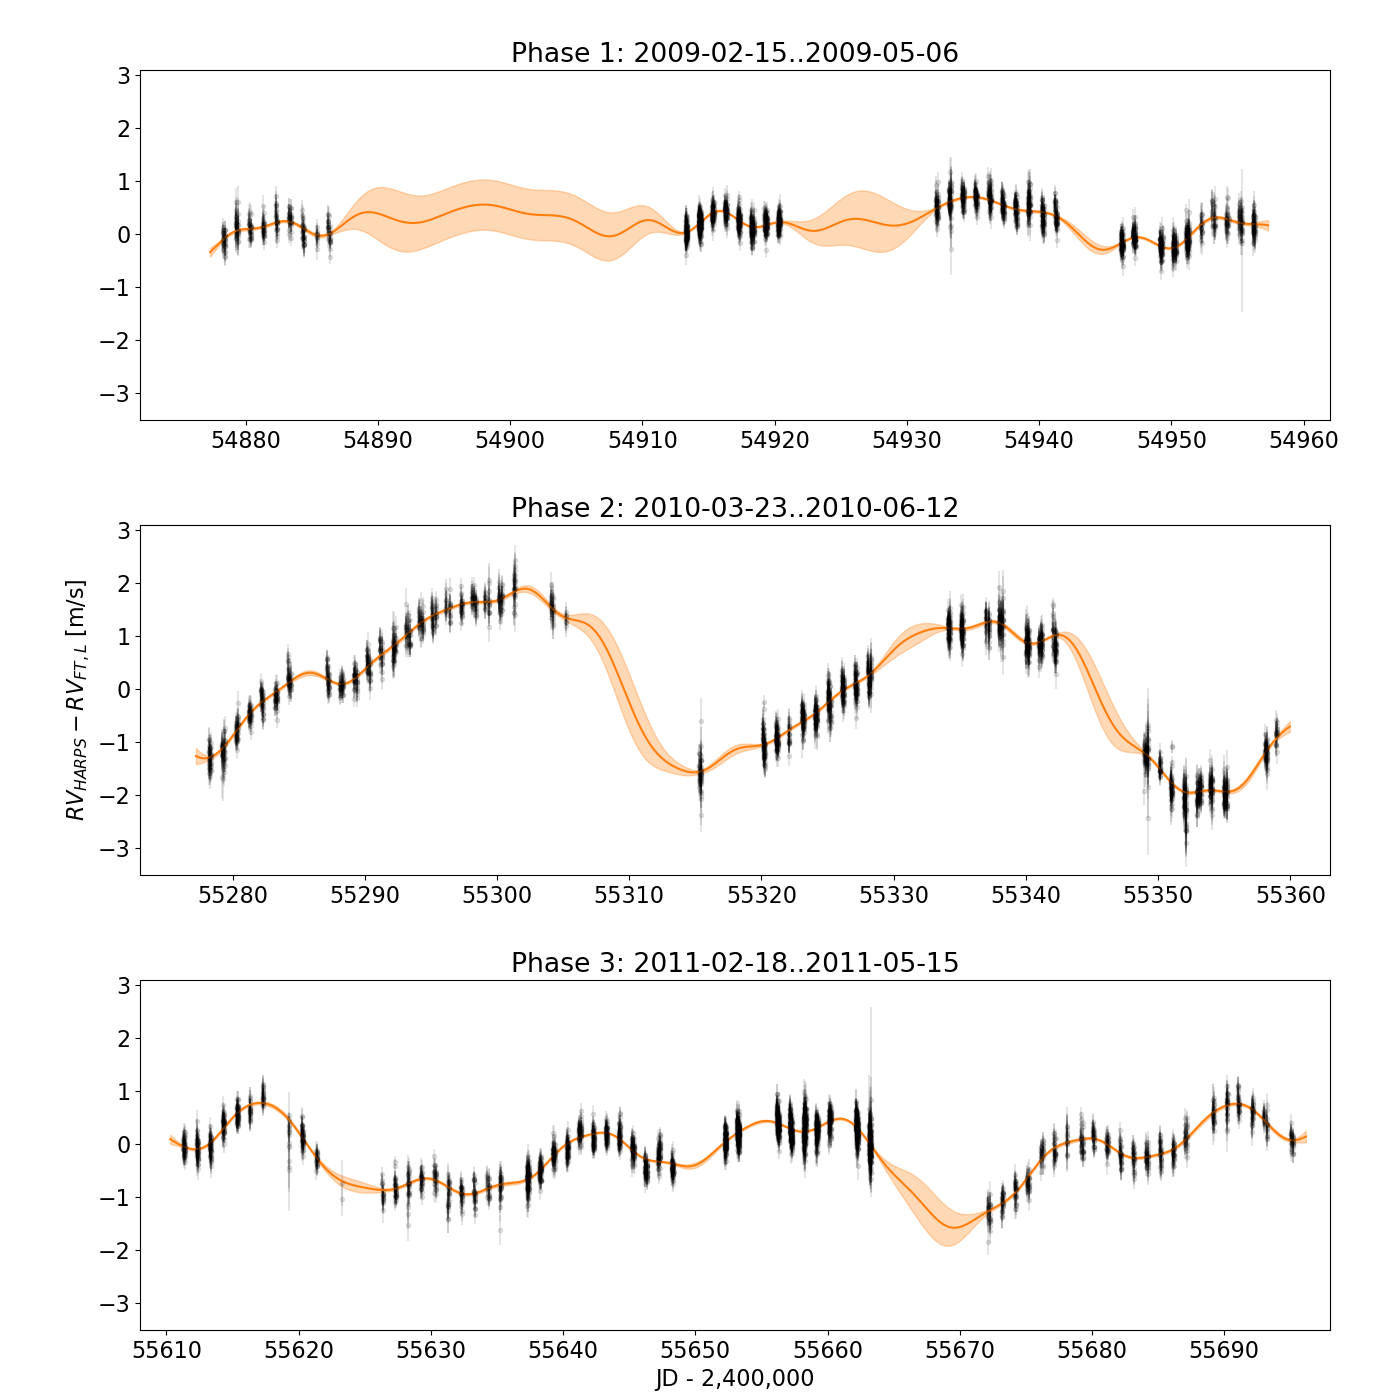
\includegraphics[width = 1.0 \linewidth]
{./Figures/Methods/Alpha_Cen_B.png}
\caption[$\alpha$ Centauri B: stellar activity analysis]
		{Stellar activity analysis of $\alpha$ Centauri B using $\mathit{\Phi}$ESTA. The scaling of the corresponding axes on all subplots are identical. Black dots (with errorbars taken as the photon noise) are the jitter metric $\Delta RV_\text{L}$; the orange solid line is the best fit solution with a quasi-periodic kernel using Gaussian processes and the shaded area is its $1\sigma$ boundary.}
\label{fig:Alpha_Cen_B}
\end{figure} 
%-------------

Fig.~\ref{fig:Alpha_Cen_B} shows that $\alpha$ Centauri B's activity level increased dramatically between 2009 (upper panel) and 2010 (middle panel), and then declined in 2011 (lower panel). In 2010, $\alpha$ Centauri B was dominated by a simple global feature on the stellar surface that appeared with a rotation period of around 40 days, while in 2009 and 2011 the star appears more likely to have been covered by various local features, producing disc inhomogeneity at smaller scales. 

We could obtain the stellar rotation period from our best fit solution with a quasi-periodic kernel in the framework of Gaussian processes. For the three epochs that we studied from 2009 to 2011, we estimate the rotation period to be 37.1, 35.70 and 36.7 days, all consistent with the pre-claimed $36.2\pm1.4$ days \cite{DeWarf2010}. In comparison, \cite{Dumusque_Centauri_B} presented the estimated rotation period to be 39.76, 37.80, 36.71 days respectively for the three years, which was obtained by fitting the radial velocity data by a long-term magnetic cycle model and a stellar rotation described by sine waves accompanied by its harmonics. Note that longer timespans of the three epochs were used by \cite{Dumusque_Centauri_B} to obtain the rotation period. 

A substantial literature has studied the rotationally modulated activity of $\alpha$ Centauri B. The prominent periodicity in 2010 that we present is found to be visually consistent with $\log (R'_\text{HK})$ in original $\alpha$ Centauri Bb discovery paper \cite{Dumusque_Centauri_B}, as well as with the equivalent widths and core flux of activity-sensitive Fe and Mg lines reported in \cite{Thompson2017MNRAS} and \cite{Wise2018}. 

In a more detailed investigation, we present the correlations among a range of existed activity indicators and our jitter metric $\Delta RV_\text{L}$ for the Epoch 2 data of the year 2010 (Fig.~\ref{fig:Correlogram_indicator}). The line core flux (i.e. depth of a line) measurements of Fe 4375.9{\AA} and half-depth range (i.e. width at half-depth flux) measurements of Fe 5250.2{\AA} were shared by \cite{Wise2018} through personal correspondence. The bisector, $\log (R'_\text{HK})$ and the full width at half maximum (FWHM) of the cross-correlation line profiles were taken from the publicized supplementary data file of \cite{Dumusque_Centauri_B}. Since indicators from different sources were binned or selected in their own unique way, we used a moving average to ``interpolate" (and at the same time smooth) all the activity indicators as well as the jitter metric $\Delta RV_\text{L}$ to the same timestamps. The two indicators -- bisector and $\Delta RV_\text{L}$, which measure the line deformation in a more direct manner with the unit of a line shift km/s -- are relatively well linearly (anti-)correlated, however, these two indicators do not show a one-to-one correlation with the other indicators studied. This may be because in some circumstances, $\log (R'_\text{HK})$, FWHM, core flux and half-depth range (as well as other indicators that measures flux changes of a line) can become degenerate. For example, while an asymmetric line profile and its mirrored counterpart can be distinguished in $\Delta RV_\text{L}$ and bisectors, they would present the same measurements in $\log (R'_\text{HK})$, FWHM, core flux, half-depth range. As a result, correlating $\Delta RV_\text{L}$ and the bisector with stellar activities would be more reasonable than correlating the $R'_\text{HK}$ activity index with the activity-induced radial velocity, as was used to construct part of the radial velocity model of $\alpha$ Centauri B in \cite{Dumusque_Centauri_B}. In spite of this, the activity indicators of $\log (R'_\text{HK})$, FWHM, core flux and half-depth range show relatively good consistency amongst themselves, especially between $\log (R'_\text{HK})$ and the line core flux. 

%-------------
\begin{figure}[tbp]
\centering
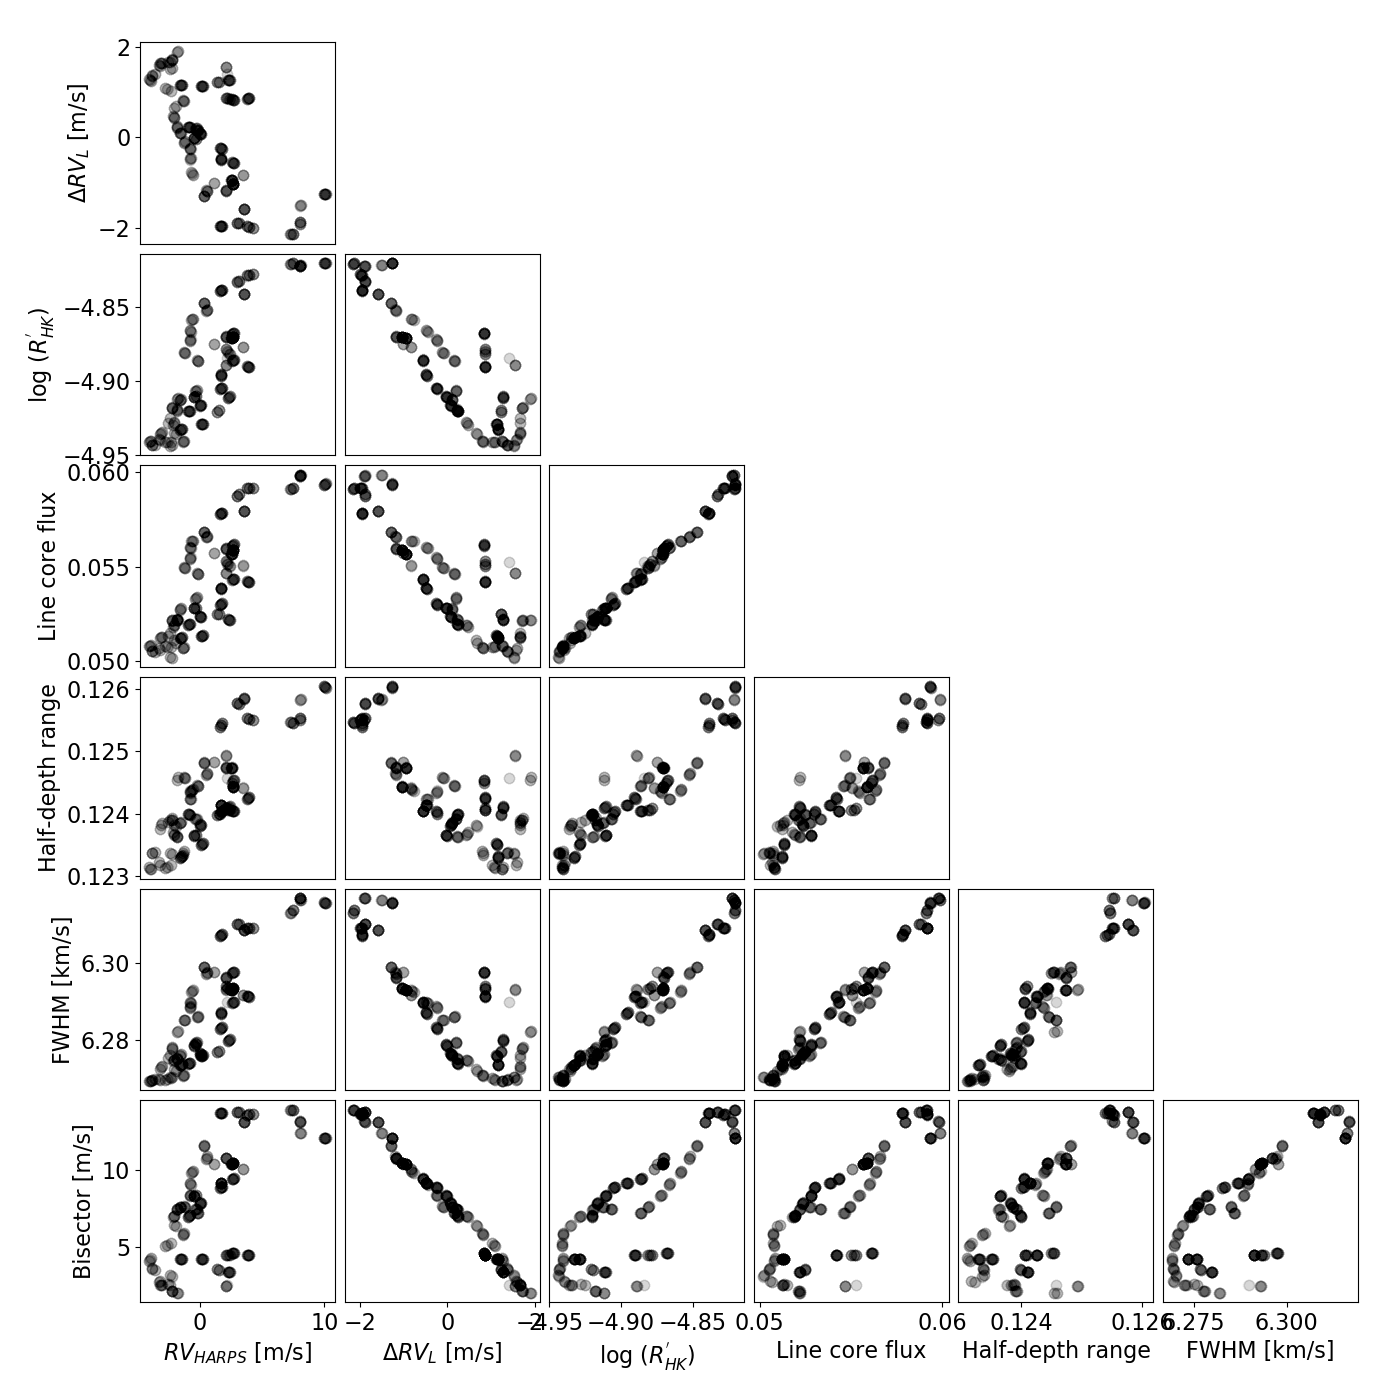
\includegraphics[width = 1.0 \linewidth]
{./Figures/Methods/Correlogram2_indicator_2010.png}
\caption[Correlations among the activity indicators and the jitter metric]
		{Correlations among the 5 activity indicators, the jitter metric $\Delta RV_\text{L}$ and the HARPS radial velocities (minus the binary stellar companion fitted by a second order polinomial) for the Epoch 2 data of $\alpha$ Centauri B in 2010. The line core flux in this plot is a measurement of the line depth of Fe 4375.9 \AA, and the half-depth range is a measurement of the line width at half-depth of Fe 5250.2 \AA, both processed based on data from \cite{Wise2018}.}
\label{fig:Correlogram_indicator}
\end{figure} 
%-------------



% While our scaled jitter correction $\Delta RV_\text{L}$ in Epoch 2 (2010) does not match with the rotational activity fit of \cite{Dumusque_Centauri_B} and \cite{Hatzes2013}, we do find some shared similarities between our $\Delta RV_\text{L}$ in Epoch 3 (2011) and the corresponding trunk of rotational activity fit presented in \cite{Dumusque_Centauri_B} and \cite{Hatzes2013}, which were obtained using completely different methods from ours. 



While , \S\ref{sec:Classification} has demonstrated $\mathit{\Phi}$ESTA does provide a quick assessment of whether a system hosts a planet / planets. 





\subsection{$\epsilon$ Eridani (HD22049)}

\subsection{$\tau$ Ceti (HD10700)}

%HD\,49933 is an F2 main sequence star with an apparent magnitude of $m_V=5.8$ (\cite{Malaroda1975}), 



%%----------------------------------------------------------------------------------------	
\pagebreak
%%----------------------------------------------------------------------------------------	
%----------------------------------------------------------------------------------------
%\clearpage
\section{References}
\label{\thesection}
\vspace{-1.5cm}
\setstretch{1.0}
\bibliographystyle{unsrt}
\bibliography{Bibliography}
\setstretch{1.3}
